
% \subsection{Track-Assisted Mass ($\mta$)}
% The track-assisted mass, $\mta$, was one of the first attempts to combine the information form the tracker system and from the calorimeter. It is defined as $\mta=\frac{p_T^{calo}}{p_T^{track}}\times m^{track}$, where the $p_T^{track}$ and the $m^{track}$ are calculated from the tracks which are associated to the large-radius jet, adding up their 4-momenta (hence exploiting the superior angular resolution of the tracker system); the $p_T^{calo}$ is the transverse momentum as measured from the calorimeter system. The ratio $p_T^{calo}/p_T^{track}$ restores the fraction of the missing neutral component in the $m^{track}$.
% The $\mta$ has a better performance on the reconstruction of boosted objects such as $W/Z$ in the extreme kinematic regime ($\sim $ 1 TeV) and above in the transverse momentum of the decaying electroweak object. Another advantage of this observable shows up as it comes to the systematic uncertainties: in particular jet mass scale and jet mass resolution uncertainty on $\mta$ can be estimated by propagating the track reconstruction uncertainties and calorimeter-jet $\pt$ uncertainties through the definition of the variable given above. The tracking uncertainties are smaller for $\mta$ rather than $\mcal$ because a larger extent of the uncertainty cancels in the ratio $m^{track}/p_T^{track}$.
% Apart all of this advantages, the track-assisted mass shows its limits when it comes to intermediate transverse momentum regimes and below ($\pt < 1 $ TeV) in $W/Z$ and for Higgs and top quarks throughout the whole kinematic space.
% % The track-assisted mass, $\mta$, was one of the first attempts to combine the information form the tracker system and from the calorimeter. 
% % The track mass is missing the neutral component, i.e. each measurement is missing the fraction $\frac{neutral+charged}{charged}$, but it has very good angular resolution but $\pt$ resolution degrades linearly with the transverse momentum. The calorimeter mass, on the other hand, has the limitation of the angular resolution of the topo-clusters but relative energy resolution increases at higher energies. The missing neutral fraction from the tracker system could be corrected on a jet-by-jet basis taking advantage of the two detector sub-system optimalities: this leads to the definition of the \textit{track-assisted mass} ($m^{TA}$):
% % \begin{equation}
%  % m^{TA}=\frac{p_T^{calo}}{p_T^{track}}\times m^{track}
% % \end{equation}
% % The better resolution of the $\mta$ takes place at the scale of above $\sim1$ TeV of transverse momentum for $W/Z$, while the performance is suboptimal to the calorimeter mass for all the other samples considered.
% % Another advantage with respect to 
% Full description of this variable is given in the ATLAS CONF Note \cite{art35}.
% % The main limitation of the calorimeter mass comes from the angular resolution of the topo-clusters, which, for extreme kinematic regimes, start approaching each other at the point that they hit the granularity of the detector. The main advantage is that on the contrary the relative energy resolution increases at higher energies.

% % The tracks instead have a very good angular resolution, but $\pt$ relative resolution degrades linearly with the transverse momentum. 

% % One could then think about creating a variable which exploits the advantages of both and minimizes the disadvantages. As seen, the track mass is missing the neutral component, i.e. each measurement is missing the fraction $\frac{neutral+charged}{charged}$, but it could be corrected on a jet-by-jet basis: this leads to the definition of the \textit{track-assisted mass} ($m^{TA}$):
% % \begin{equation}
% %  m^{TA}=\frac{p_T^{calo}}{p_T^{track}}\times m^{track}
% % \end{equation}

% % It can be intuitively understood as follows: the term $m^{track}$ has the superior angular resolution, but misses the neutral component; the ratio $p_T^{calo}/p_T^{track}$, representing exactly the $(neutral+charged)/charged$ ratio, ``restores'' the correct value of the mass back to $charged+neutral$.
% % \begin{figure}[!ht]
% %   \centering
% %       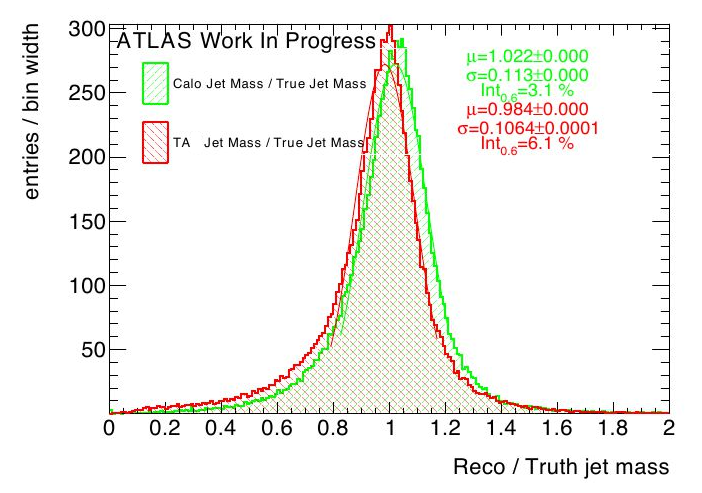
\includegraphics[width=0.7\textwidth]{jet_part/mta/allbinptmta.png}
% %   \caption[$\mcal$ and $\mta$ mass responses]{Track-assisted mass response plot for boosted $W/Z$: in green the calorimeter mass, in red the track-assisted mass. On the right are shown properties of the fit to the Gaussian core; it can be seen than the width of the $\mta$ distribution is smaller, and the mean is slightly below the calorimeter mass.}
% %   \label{fig:mta1}
% % \end{figure}

% % From Figure \ref{fig:mta1} the comparison of the track-assisted mass and the calorimeter mass; the width of the distribution is smaller, making this observable a good candidate for usage.


% % \subsection{Advantages and Limitation of $\mta$}
% % The $\mta$ has a good handle on boosted $W/Z$, looking at all the transverse momentum spectrum for these results.

% % \begin{figure}[!ht]
% %   \centering
% %       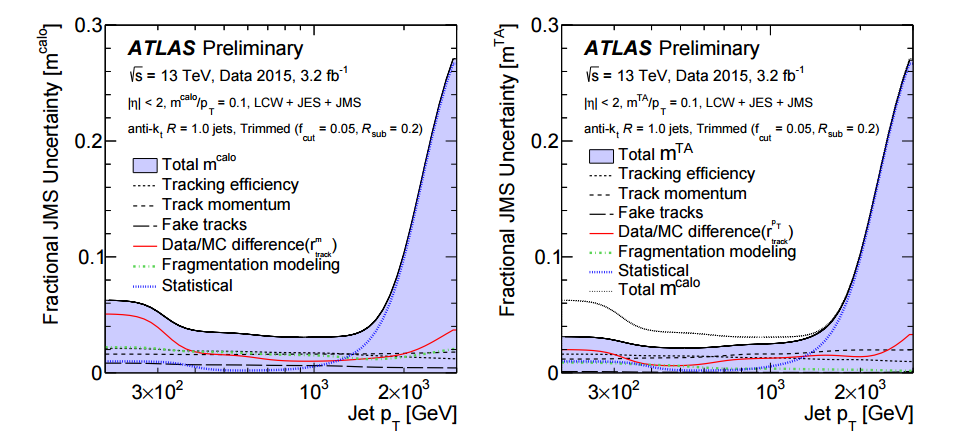
\includegraphics[width=0.9\textwidth]{jet_part/uncert.png}
% %   \caption[Comparison of the uncertainties for $\mcal$ and $\mta$]{Comparison of the uncertainties for $\mcal$, on the left, and $\mta$, on the right the rise on the high jet $\pt$ is due to statistics. From the \cite{art35}.}
% %   \label{fig:uncert}
% % \end{figure}

% % Another big advantage which supports the use of the track-assisted mass is the relatively small uncertainties: in Figure \ref{fig:uncert} the comparison of $\mcal$ (left) and $\mta$ (right) fractional uncertainties on the JMS, shows how the tracking uncertainties are much smaller because of the ratio $m^{track}/p_T^{track}$. On the right plot the black line indicates the JMS fractional uncertainty for the $\mcal$, and is always above the $\mta$. Of course this introduces another argument in the development of new techniques, which is to look for a good balance between performance and small uncertainties: a perfect observable in terms of behavior which has very big uncertainties is not really useful.


% % When looking in the extreme kinematic regime, at very high $\pt$, as in the top plot in Figure \ref{fig:mta2}, the $\mta$ shows its real strength, achieving much smaller value of the IQnR.
% % However, there are some severe limitations which are worth noting, especially looking at the performance in different regions of transverse momentum: this is shown in the bottom plot of Figure \ref{fig:mta2}, where at a low $\pt$ it exhibits a much worse behavior.

% % \subsubsection{Performance in $W \to q'\bar{q}$ Decays}

% % \begin{figure}
% %     \centering
% %     \begin{subfigure}[b]{0.5\textwidth}
% % 	\centering
% %         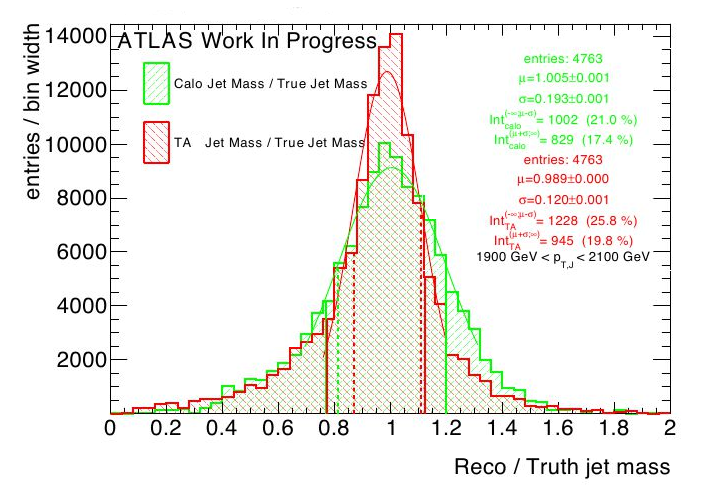
\includegraphics[width=\textwidth]{jet_part/mta/highptmta.png}
   
% % %         \label{fig:tiger}
% %     \end{subfigure}
% %     \begin{subfigure}[b]{0.5\textwidth}
% % 	\centering
% %         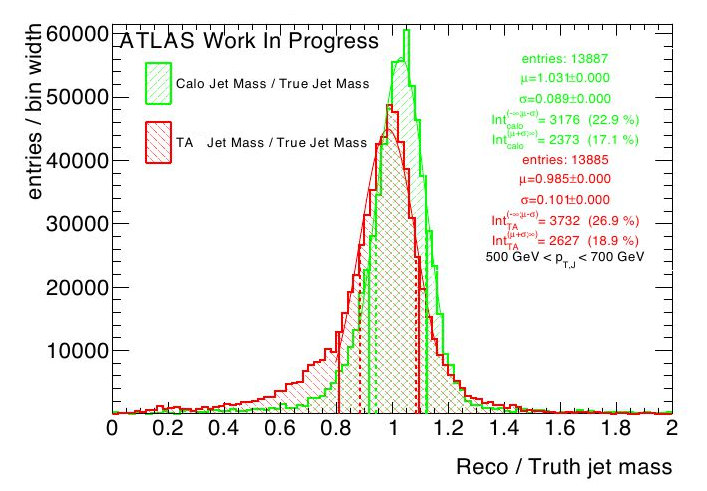
\includegraphics[width=\textwidth]{jet_part/mta/lowptmta.png}
 
% % %         \label{fig:gull}
% %     \end{subfigure}
% %     \caption[Mass response plots for the $\mta$]{Mass response plots for selected ranges of $\pt$: on the bottom, a ``low'' range, 500 GeV $<\pt<$ 700 GeV, on the top an high $\pt$, 1900 GeV $<\pt<$ 2100 GeV. A difference in performance can be clearly seen.} 
% %     \label{fig:mta2}
% % \end{figure}


% % The performance in all the bins of $\pt$ can be studied looking at Figure \ref{fig:mta3}; these plots have as horizontal axis the transverse momentum and as vertical one the value of the $\iqr$ calculated from the correspondingly response. For $W/Z$ jets, there is a crossing point around $\pt\sim$1 TeV, which can be understood as the point in which the two sub-jet present start merging (sub-jet multiplicity shown in Figure \ref{fig:multi} in Appendix).



% % \subsubsection{Performance in $t\to q'\bar{q}b$ Decays}

% % For top quarks the situation is much different: with respect to $W/Z$ jets, in fact, there are two main disparities: on one side, the mass of the top quark is much higher than the one of the electroweak bosons, hence making the separation $\Delta R=\frac{2m}{\pt}$ bigger; on the other side, the decay is not anymore two-prong (two-sub-jet-like) but rather a three-prong  (three-sub-jet-like) decay, one from the b-jet and the other two from the $W$ decay.
% % $\mta$ is here never performing better than $\mcal$, as can be seen e.g. in Figure \ref{fig:mta3}, right.


% % \begin{figure}[!ht]
% %   \centering
% %       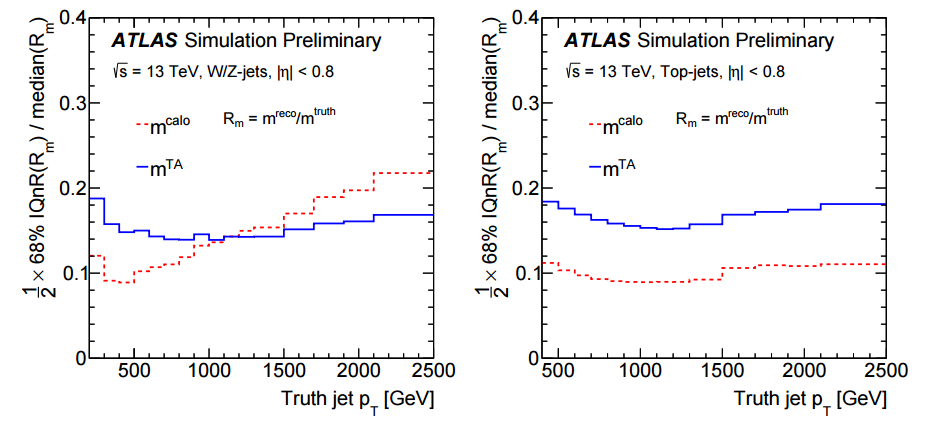
\includegraphics[width=\textwidth]{jet_part/mtawandtop.png}
% %   \caption[$m^{calo}$ and $m^{TA}$ comparison for $W/Z$ jets and top jets]{The comparison between the performance of $m^{calo}$ and $m^{TA}$ for $W/Z$ jets (left) and top jets (right); on the x-axis the transverse momentum and on the y-axes the $\iqr$ of the mass distribution, from \cite{art35}. A better observable has lower values on the y-axis. }
% %   \label{fig:mta3}
% % \end{figure}

% % \subsubsection{Performance in $h\to b\bar{b}$ Decays}

% % For boosted Higgs the $\mcal$ outperforms the $\mta$ in the spectrum of transverse momentum. Although the decay is two-pronged, the mass of the Higgs is higher than the electroweak bosons, moreover another difference lays in light quarks initiated jets and heavy quarks initiated ones, like the b-quarks from Higgs decay.
% % % the b-jet poses an additional complication which comes from the branching ratio of B mesons to muons, which leave very little energy in the calorimeter system but additional tracks.

% % \begin{figure}[!ht]
% %   \centering
% %       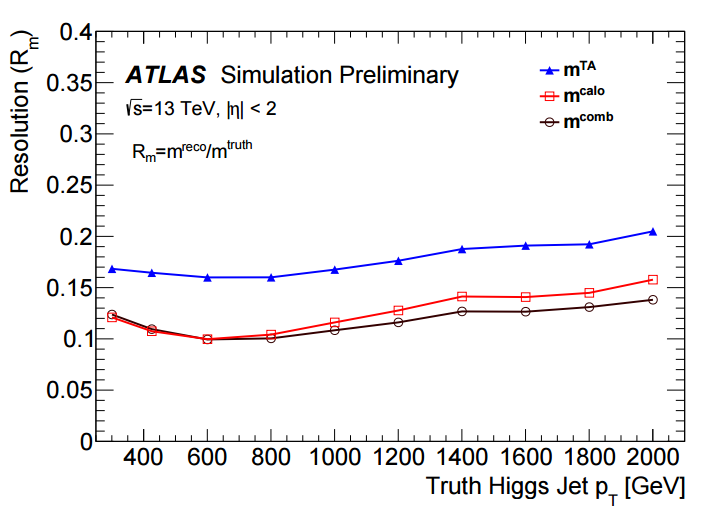
\includegraphics[width=0.7\textwidth]{jet_part/mta/higgsmta.png}
% %   \caption[Performance of the $\mta$ with the boosted Higgs sample]{Performance of the $\mta$ with the boosted Higgs sample; the $\mta$ is the blue line, the $\mcomb$ will be described later in this chapter. From \cite{art39}. The FoM here is the resolution of the Response.}
% %   \label{fig:mta4}
% % \end{figure}



% \subsection{The Track-Assisted Sub-jet Mass ($\mtas$)}
% In this section the main outcome of the optimization of the large-radius jet mas reconstruction is presented: the \textit{track-assisted sub-jet mass} ($\mtas$).
% The main idea takes inspiration from the track-assisted mass: if one can use tracks to exploit the better angular resolution and correct the missing neutral component jet-by-jet, there is an additional information that can be used. The neutral fraction, in fact, varies stochastically not only per-jet basis, but even per-sub-jet basis, since the each quark follows a different parton showering and hadronization process.
% Correcting the missed neutral component per-sub-jet, it should perform better already at an intuitive level, as it accesses information from jet substructure.
% There are few question in the definition of this mass observable, whose answers are in the next section:
% \begin{itemize}
%   \item Regarding the inputs:
%   \begin{itemize}
%      \item How to select the set of tracks to be used?
%      \item Which kind of sub-jet should be used?
%   \end{itemize}
%   \item Regarding the procedure
%   \begin{itemize}
  
%   \item How to associate the tracks to a sub-jet?
%   \item How to correct for the missed neutrals on a sub-jet basis?
%   \item How to add everything back together?
%  \end{itemize} 
 
% \end{itemize}

% Those details are given in the next subsection.


% \subsection{Observable Definition: Inputs}
% There are two inputs to the $\mtas$: tracks and sub-jets. The definition of the standard inputs are give here; alternative approaches are given in subsection \ref{sec:alternate}.

% \subsubsection{Tracks}
% Only the tracks that satisfy the quality criteria and primary vertex association, described in the appendix \ref{sec:tracks}, are used.
% The tracks are additionally required to be ghost associated to the sub-jets of the groomed jet; namely only the sub-jets which survived the trimming procedure and are described in the next subsection.
% Ghost association provides a clear correspondence of tracks to the sub-jets set and was therefore chosen and preferred to other kind of assignments.

% \subsubsection{Sub-jets}

% The choice of sub-jets must follow a simple requirement: of course we want to take those which most likely come from the hard-scattering. This means that the choice of taking them after grooming is strongly favored.

% As grooming technique used, the trimming was preferred as being the standard in ATLAS and the most flexible one for optimization studies.

% The standard version of the trimming uses the k$_t$ reclustering algorithm with radius of 0.2, with the transverse momentum ratio $f_{cut}$ at 5\%.

% As shown later, this is also the optimal configuration for sub-jets.

% \subsection{Observable Definition: Procedure}
% Having tracks and sub-jets now well defined, we can describe the recipe to produce the $\mtas$. For brevity we will call the sub-jets SJ in the formulae below. 

% As said, the tracks are the ones ghost-associated to the sub-jets; however, tracks which fall inside the area of the large-$R$ jet, but not inside the sub-jets area, are still much probably coming from the hard-scattering. They are then associated again to the closest sub-jets via $\Delta R$ association.

% Each sub-jet will have at this point some tracks associated via ghost-association and some other via $\Delta R$ (which are maximally 5\%). We call this set of tracks, a ``custom'' Track-Jet or TJ.

% At this point, the one-to-one correspondence is preserved (for each SJ there is one and only one TJ), and we can move on correcting the neutral fraction.

% Getting inspired from the formula $m^{TA}=p_T^{calo}/p_T^{track}\times m^{track}$, we would like to replicate this at sub-jet level, i.e.

% $$\mtas="\sum_{SJ}"\frac{p_T^{SJ}}{p_T^{TJ}}\times m^{TJ}$$

% Where the summation symbol between quotation mark symbolize that the sum must be intended at 4-vector level: since now we are working inside the sub-jets, in fact, we need to change the sub-jet's 4-vector itself and not only the mass. If we call $p_\mu^{TJ}$ the Lorentz vector of the track-jet, 

% $$p_\mu^{TJ} = \spvec{m^{TJ};p_T^{TJ};\eta^{TJ};\phi^{TJ}} \to p_\mu^{TA}=\spvec{m^{TJ}\times\frac{p_T^{SJ}}{p_T^{TJ}} ;p_T^{SJ};\eta^{TJ};\phi^{TJ}} $$
 
% where $p_\mu^{TA}$ is the track-assisted sub-jet's 4-vector. If we label $i$ the $i$-th track-jet of the $N$ ones present in the large-$R$ jet,

% $$ \mtas=\sqrt{\left(\sum_i^N p^{TA} \right)_\mu \left(\sum_i^N p^{TA} \right)^{_\mu}} $$
 
% \begin{figure}[!ht]
%   \centering
%       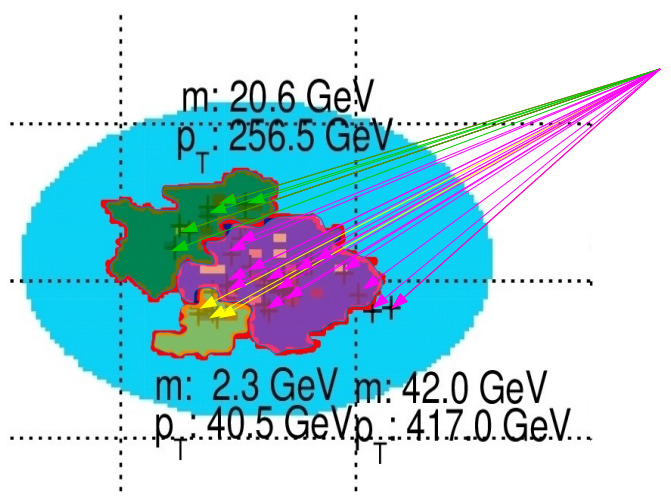
\includegraphics[width=0.6\textwidth]{jet_part/mtas/mtas.png}
%   \caption[Pictorial event display]{Pictorial event display showing the $\eta$ $\phi$ region of a large-$R$ anti-k$_t$ trimmed jet, (in blue the catchment area of the anti-k$_t$) showing the different k$_t$ sub-jets: they are highlighted in green, fuchsia and yellow. The associated track-jets (here indicated as arrows pointing the calorimeter area) are colored with the same color of the correspondent sub-jet. Some tracks associated with $\Delta R$ procedure can be seen in the fuchsia sub-jet. The transverse momenta and mass values are also shown for the sub-jets.}
%   \label{fig:mtas1}
% \end{figure}

% An important remark is that, in the case of a large-$R$ jet with only one sub-jet, the $\mtas$ has exactly the same definition of the $\mta$. This implies, since the angular separation of the decay product scales inversely with $\pt$, that the performance should approach the one of the $\mta$ at very high transverse momenta. However, the space for improvement is precisely in the low-intermediate $\pt$ regime.

\subsection{Performance in $W \to q'\bar{q}$ Decays}
The $W/Z$ decay was the first one looked at, and with which the $\mtas$ was designed. The $\mcal$ shows a fast deterioration of the performance at high $\pt$, and, as shown in the previous section, the $\mta$ prevents this deterioration but suffers at low transverse momenta ($\pt<1$ TeV).
The $\mtas$ has a similar behavior in the extreme transverse momentum regime as the $\mta$, since the sub-jet multiplicity peaks at one, where there are no differences between the two observables.
In the low-$\pt$ regime, on the contrary, it exploits the difference in charged to neutral ratio for each sub-jet, achieving a better performance.
This is shown in Figure \ref{fig:mtas2} as a function of $\pt$: below $\sim$ 1 TeV achieves lower values of the IQnR converging from below to the $\mta$ as the number of sub-jets decreases to one.

% \begin{figure}[!ht]
%   \centering
%       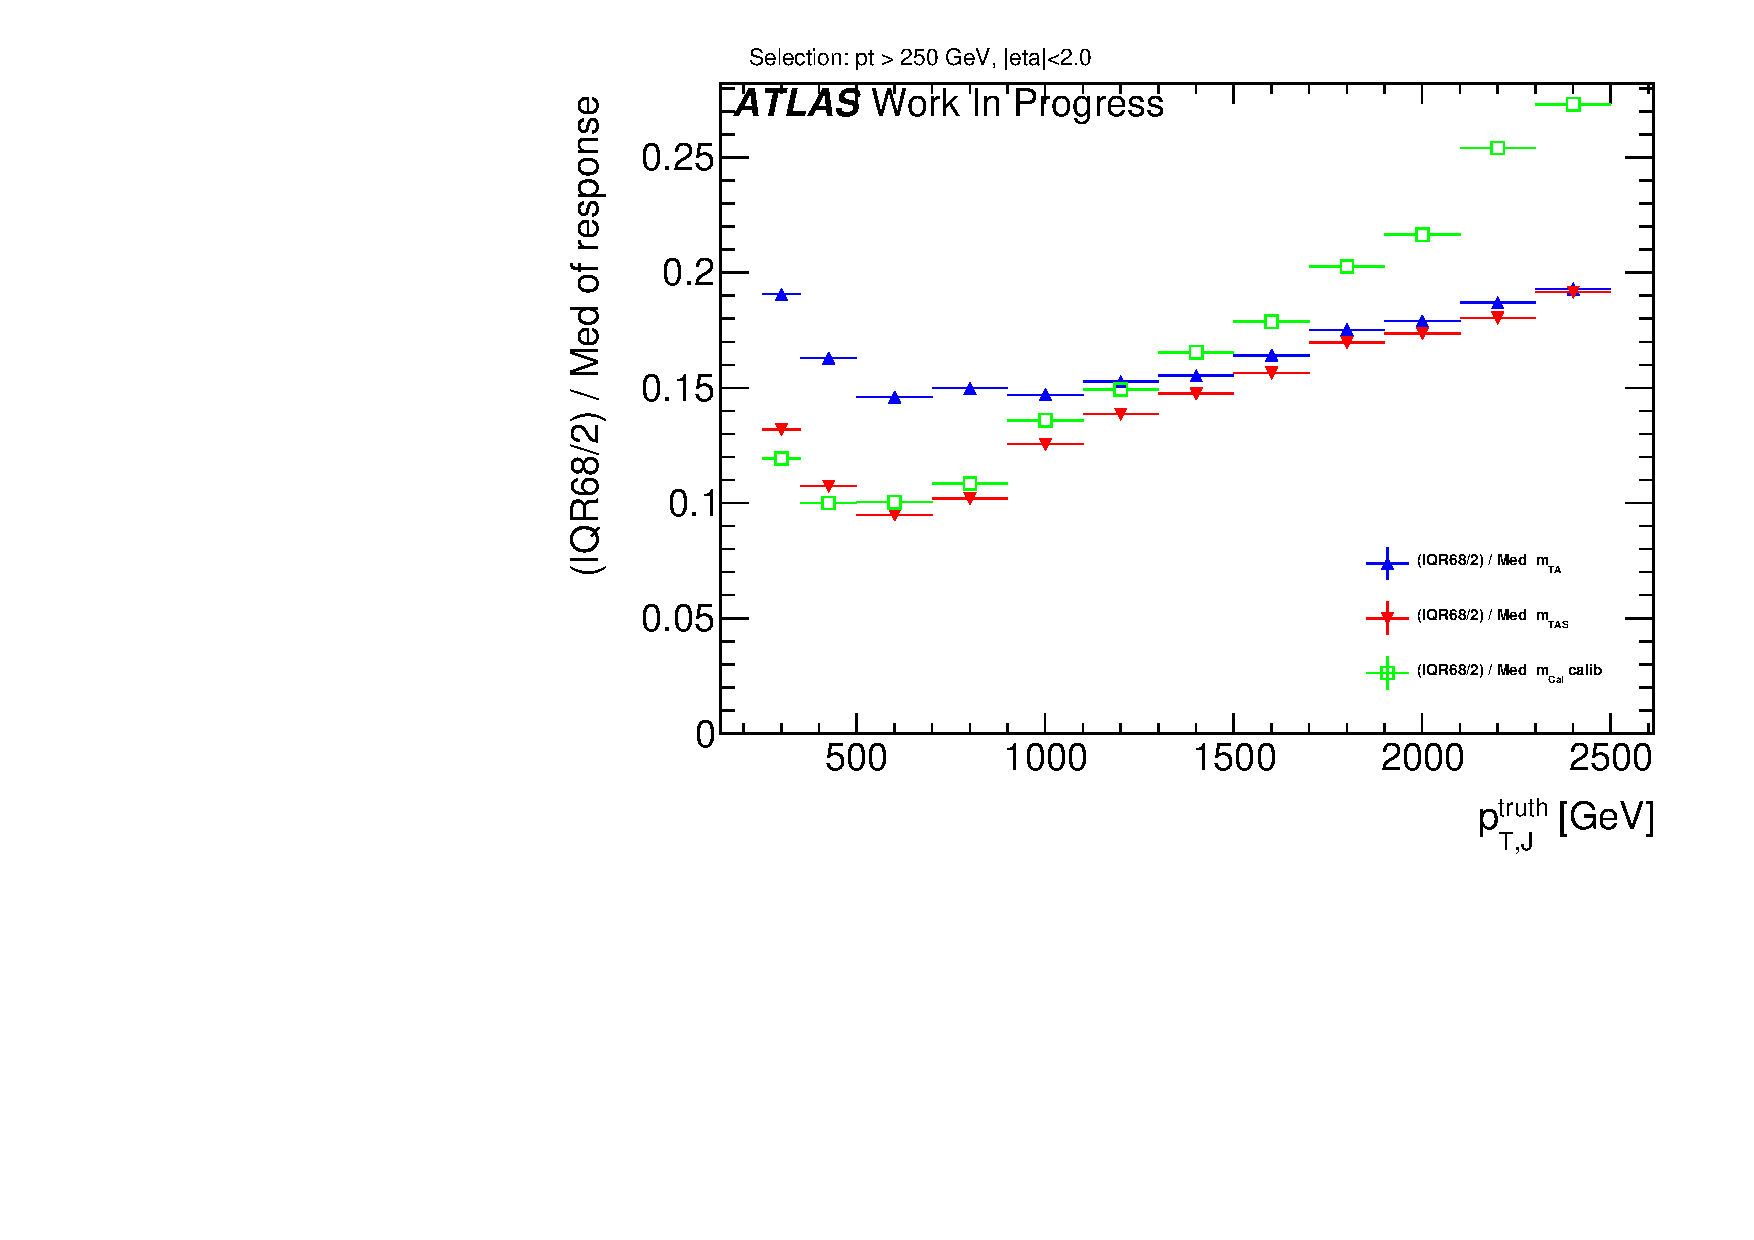
\includegraphics[width=0.7\textwidth]{jet_part/mtas/71graphcftr_h_JetRatio_mJ12CALOIQRoMWZ.pdf}
%   \caption[$\mtas$ for boosted $W/Z$]{Performance of the $\mtas$ versus the $\mcal$ and $\mta$ for the boosted $W/Z$ sample.}
%   \label{fig:mtas2}
% \end{figure}


\subsection{Performance in $h\to b\bar{b}$ Decays}
In the Randall-Sundrum graviton to di-Higgs to four b-quark, the performance is again problematic for the $\mta$ with respect to $\mcal$, which is far beyond the latter, while the performance of the $\mtas$ is partially similar to the top-quark decay, but degrades much more in the extreme $\pt$ regime, following the $\mta$. Shown in Figure \ref{fig:mtas4}.

\begin{figure}
    \centering
    \begin{subfigure}[b]{0.45\textwidth}
  \centering
      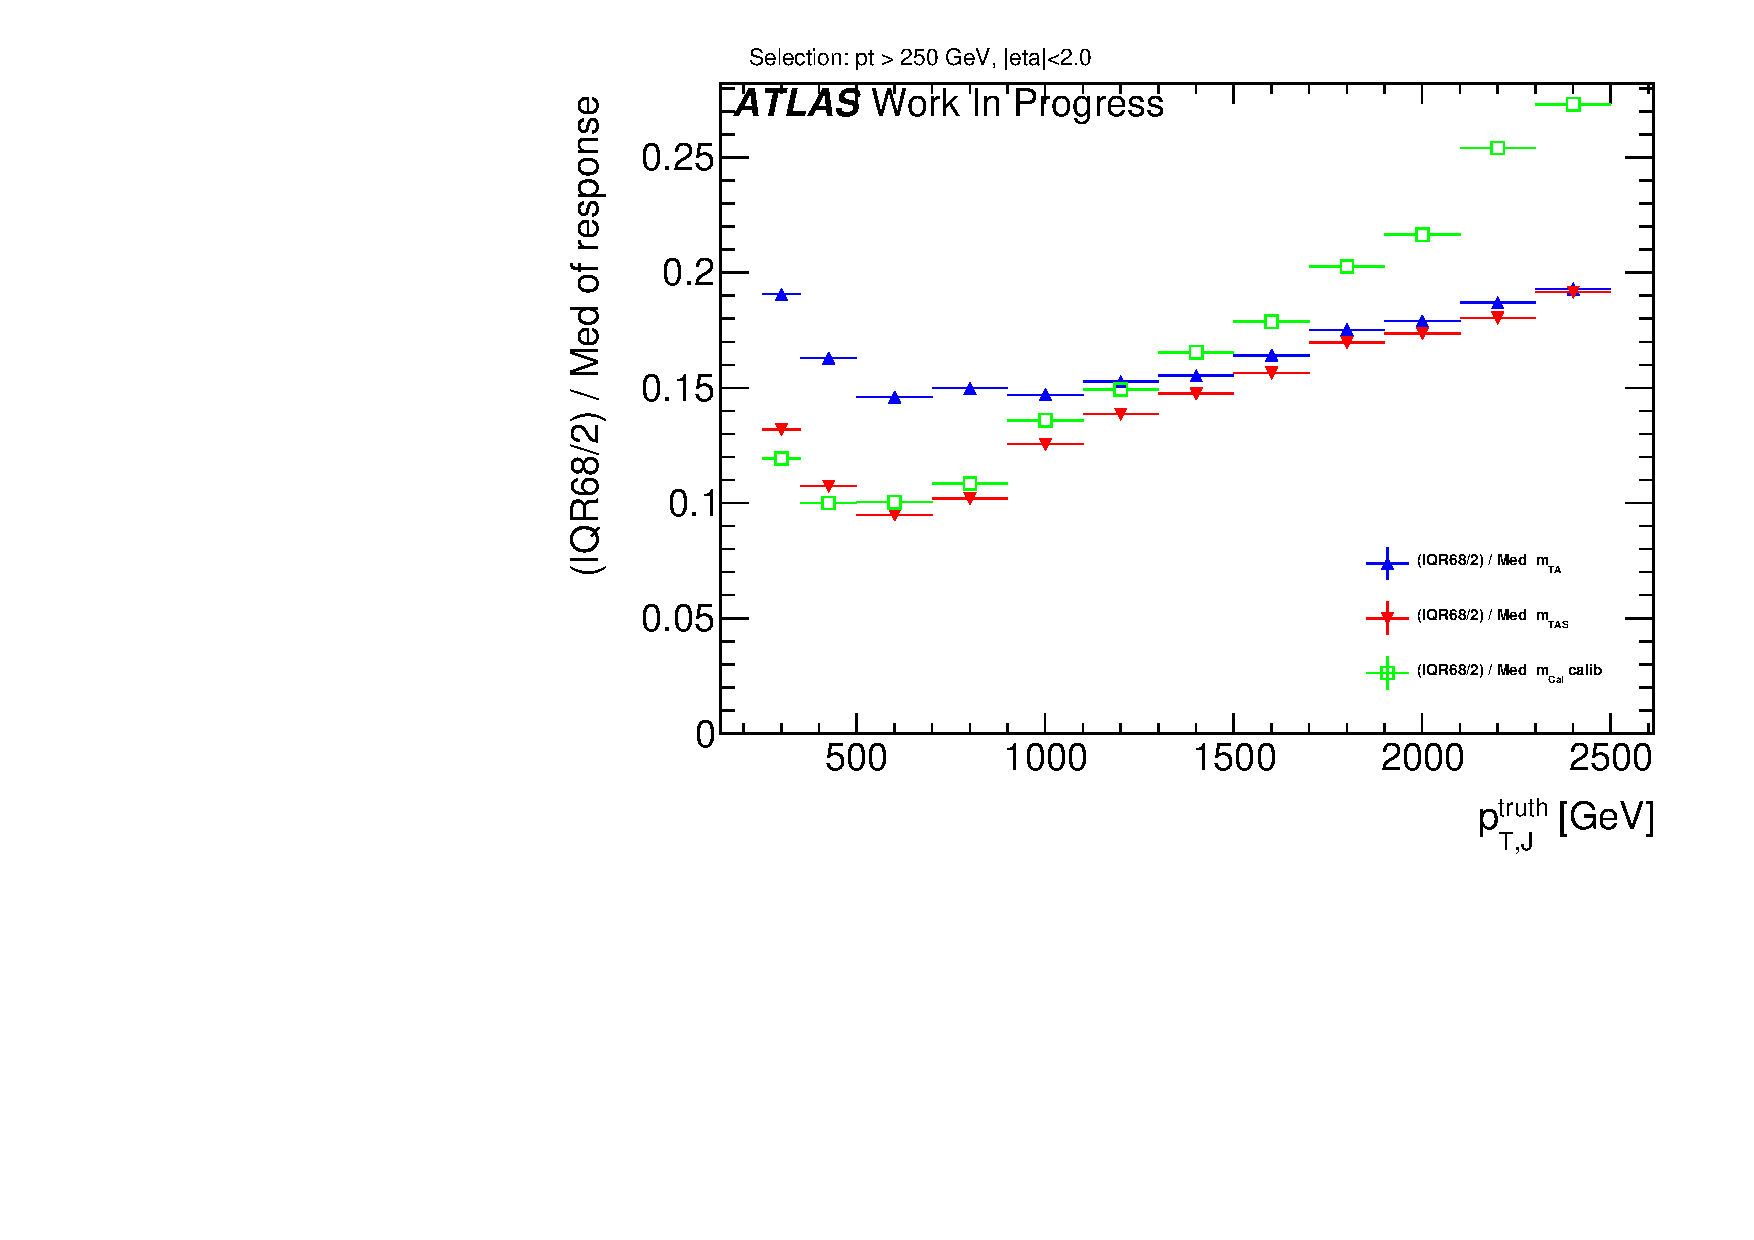
\includegraphics[width=0.9\textwidth]{jet_part/mtas/71graphcftr_h_JetRatio_mJ12CALOIQRoMWZ.pdf}
  \caption[$\mtas$ for boosted $W/Z$]{$W/Z$ jets.}
  \label{fig:mtas2}
    \end{subfigure}%
    \begin{subfigure}[b]{0.45\textwidth}
  \centering
      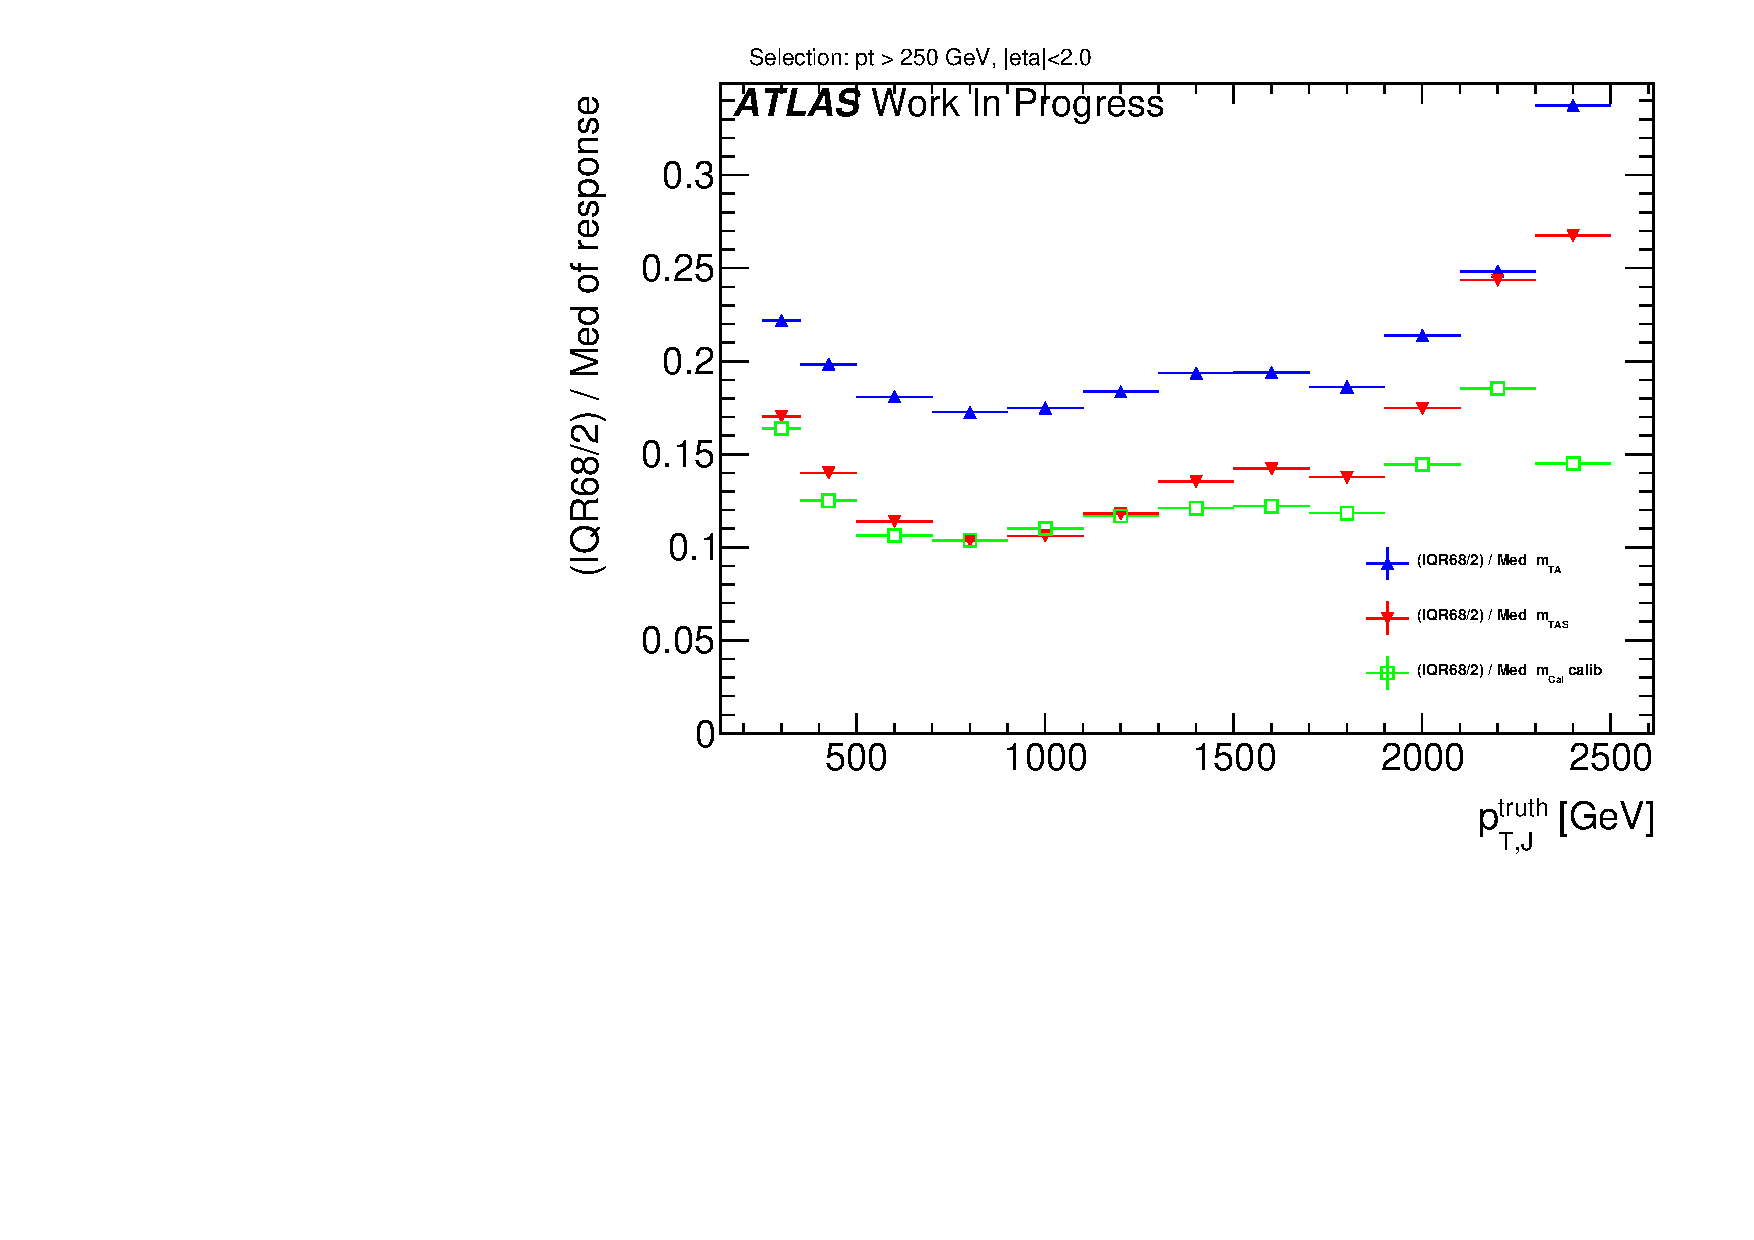
\includegraphics[width=0.9\textwidth]{jet_part/mtas/71graphcftr_h_JetRatio_mJ12CALOIQRoMHiggs.pdf}
  \caption[$\mtas$ for boosted Higgs]{Higgs jets.}
  \label{fig:mtas4}
    \end{subfigure}
 \begin{subfigure}[b]{0.45\textwidth}
  \centering
      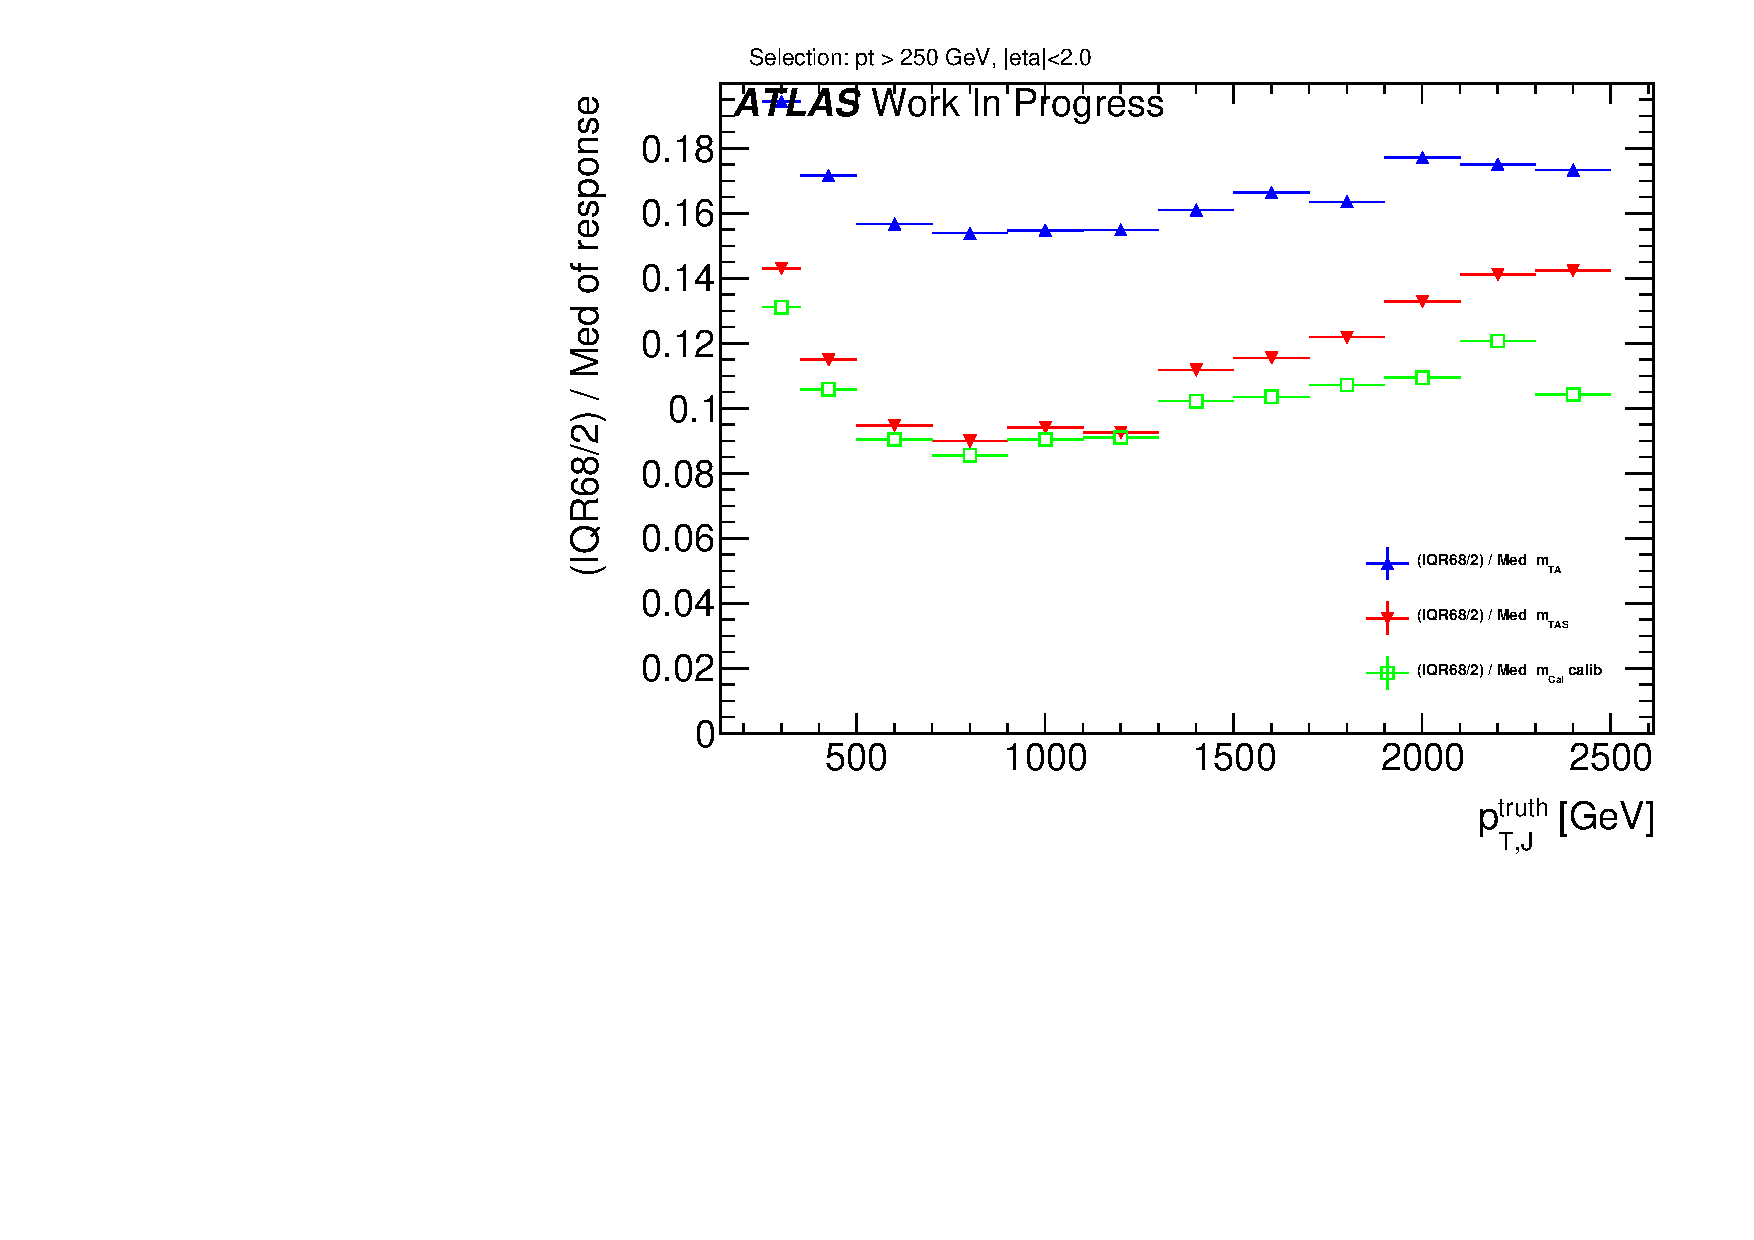
\includegraphics[width=0.9\textwidth]{jet_part/mtas/71graphcftr_h_JetRatio_mJ12CALOIQRoMTops.pdf}
  \caption[$\mtas$ for boosted tops]{Top jets.}
  \label{fig:mtas3}
    \end{subfigure}%


    \caption[Performance of the $\mtas$ versus the $\mcal$ and $\mta$]{Performance of the $\mtas$ versus the $\mcal$ and $\mta$ for $W/Z$, top left, where $\mta$ is not better than $\mcal$ in the low $\pt$ range but is outperformed by the $\mtas$;  Higgs decay, where $\mcal$ is everywhere better than $\mta$, yet comparable with $\mtas$ and top decays where the more complex topology makes critical the high $\pt$ regime} 
    % \label{fig:meanandtail}
\end{figure}


\subsection{Performance in $t\to q'\bar{q}b$ Decays}
The top decays are shown on Figure \ref{fig:mtas3}; the $\mtas$ is comparable yet slightly worse than the $\mcal$ in the low-middle $\pt$ regime, while degrades at higher $\pt$ approaching the $\mta$, which is far beyond the track-assisted sub-jet mass in performance.
As already noted, the worse performance can be ascribed both to the higher top-quark mass, and to its different and more complex decay topology.


% \begin{figure}[!ht]
%   \centering
%       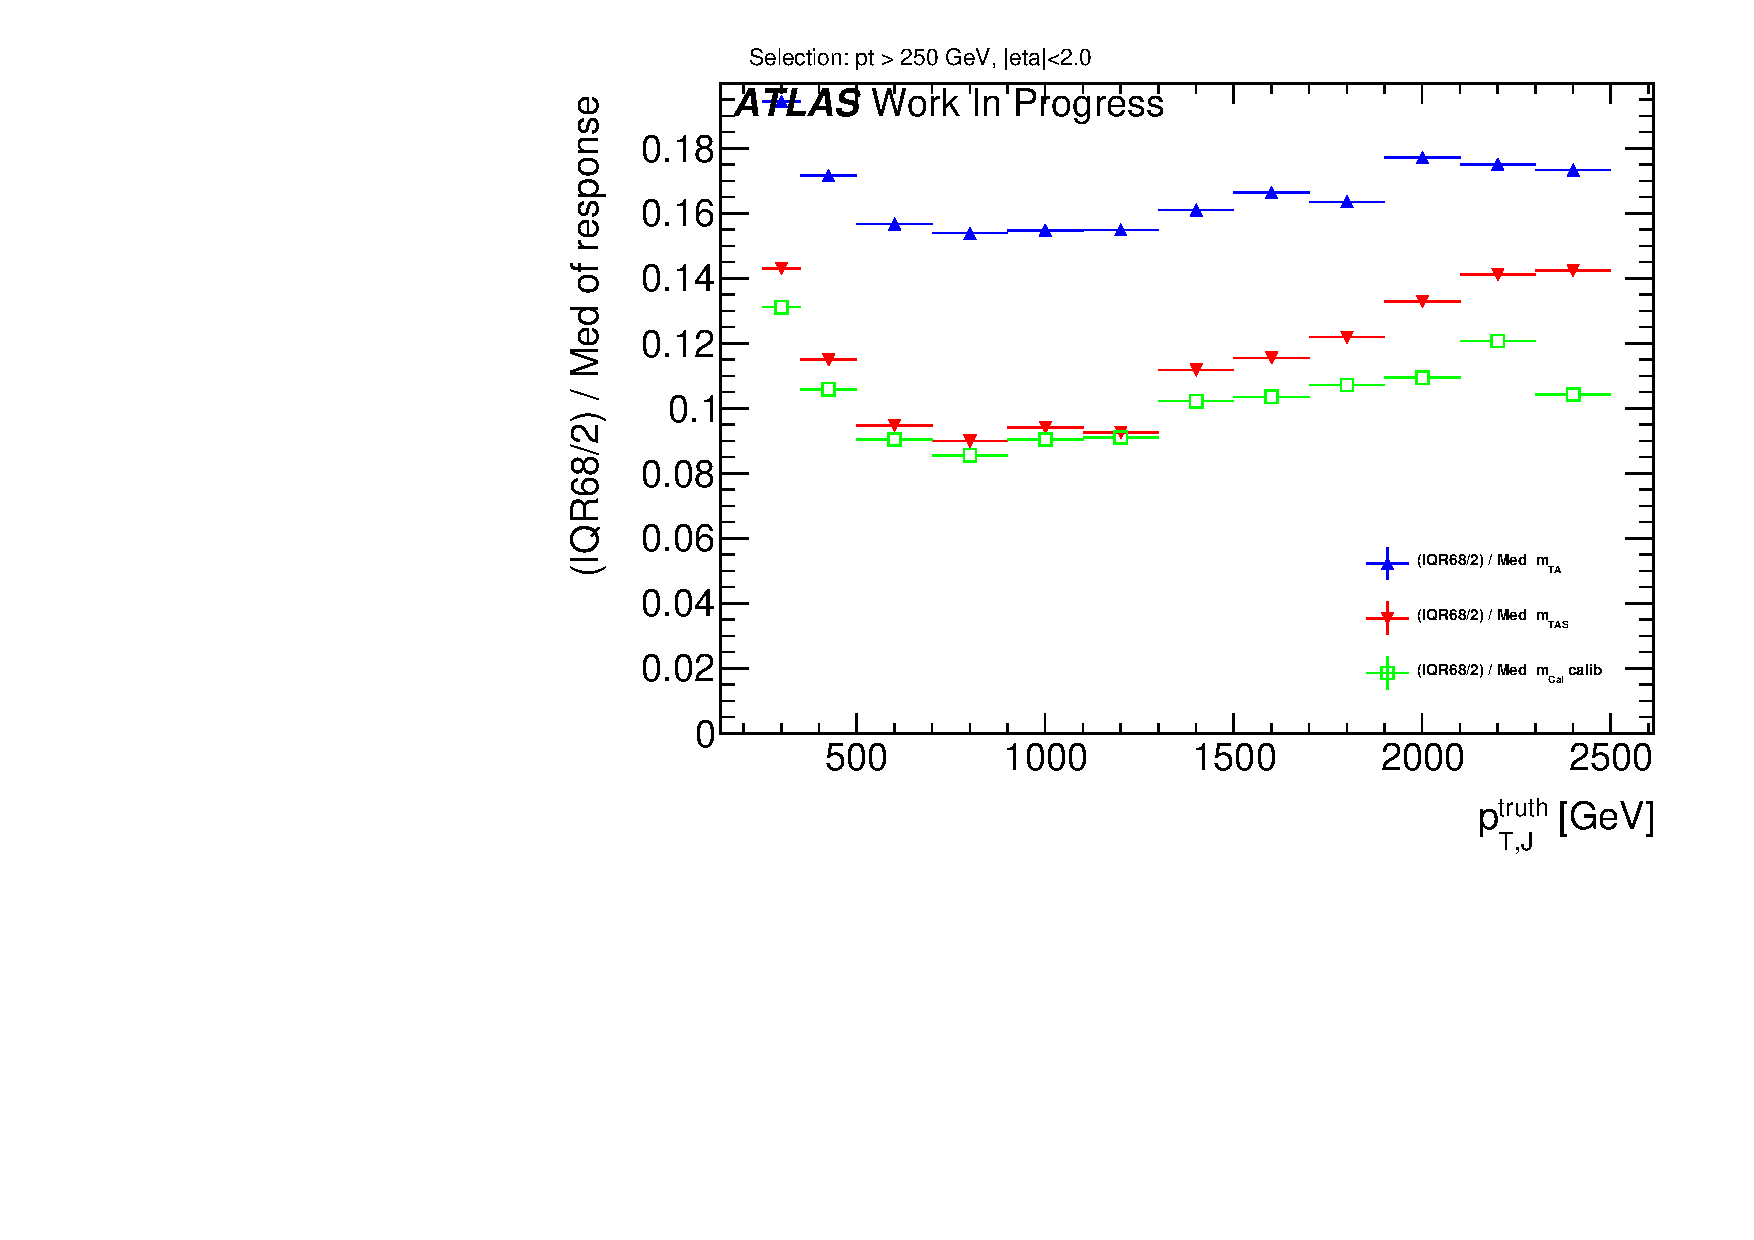
\includegraphics[width=0.7\textwidth]{jet_part/mtas/71graphcftr_h_JetRatio_mJ12CALOIQRoMTops.pdf}
%   \caption[$\mtas$ for boosted tops]{Performance of the $\mtas$ versus the $\mcal$ and $\mta$ for the boosted top sample.}
%   \label{fig:mtas3}
% \end{figure}


% \begin{figure}[!ht]
%   \centering
%       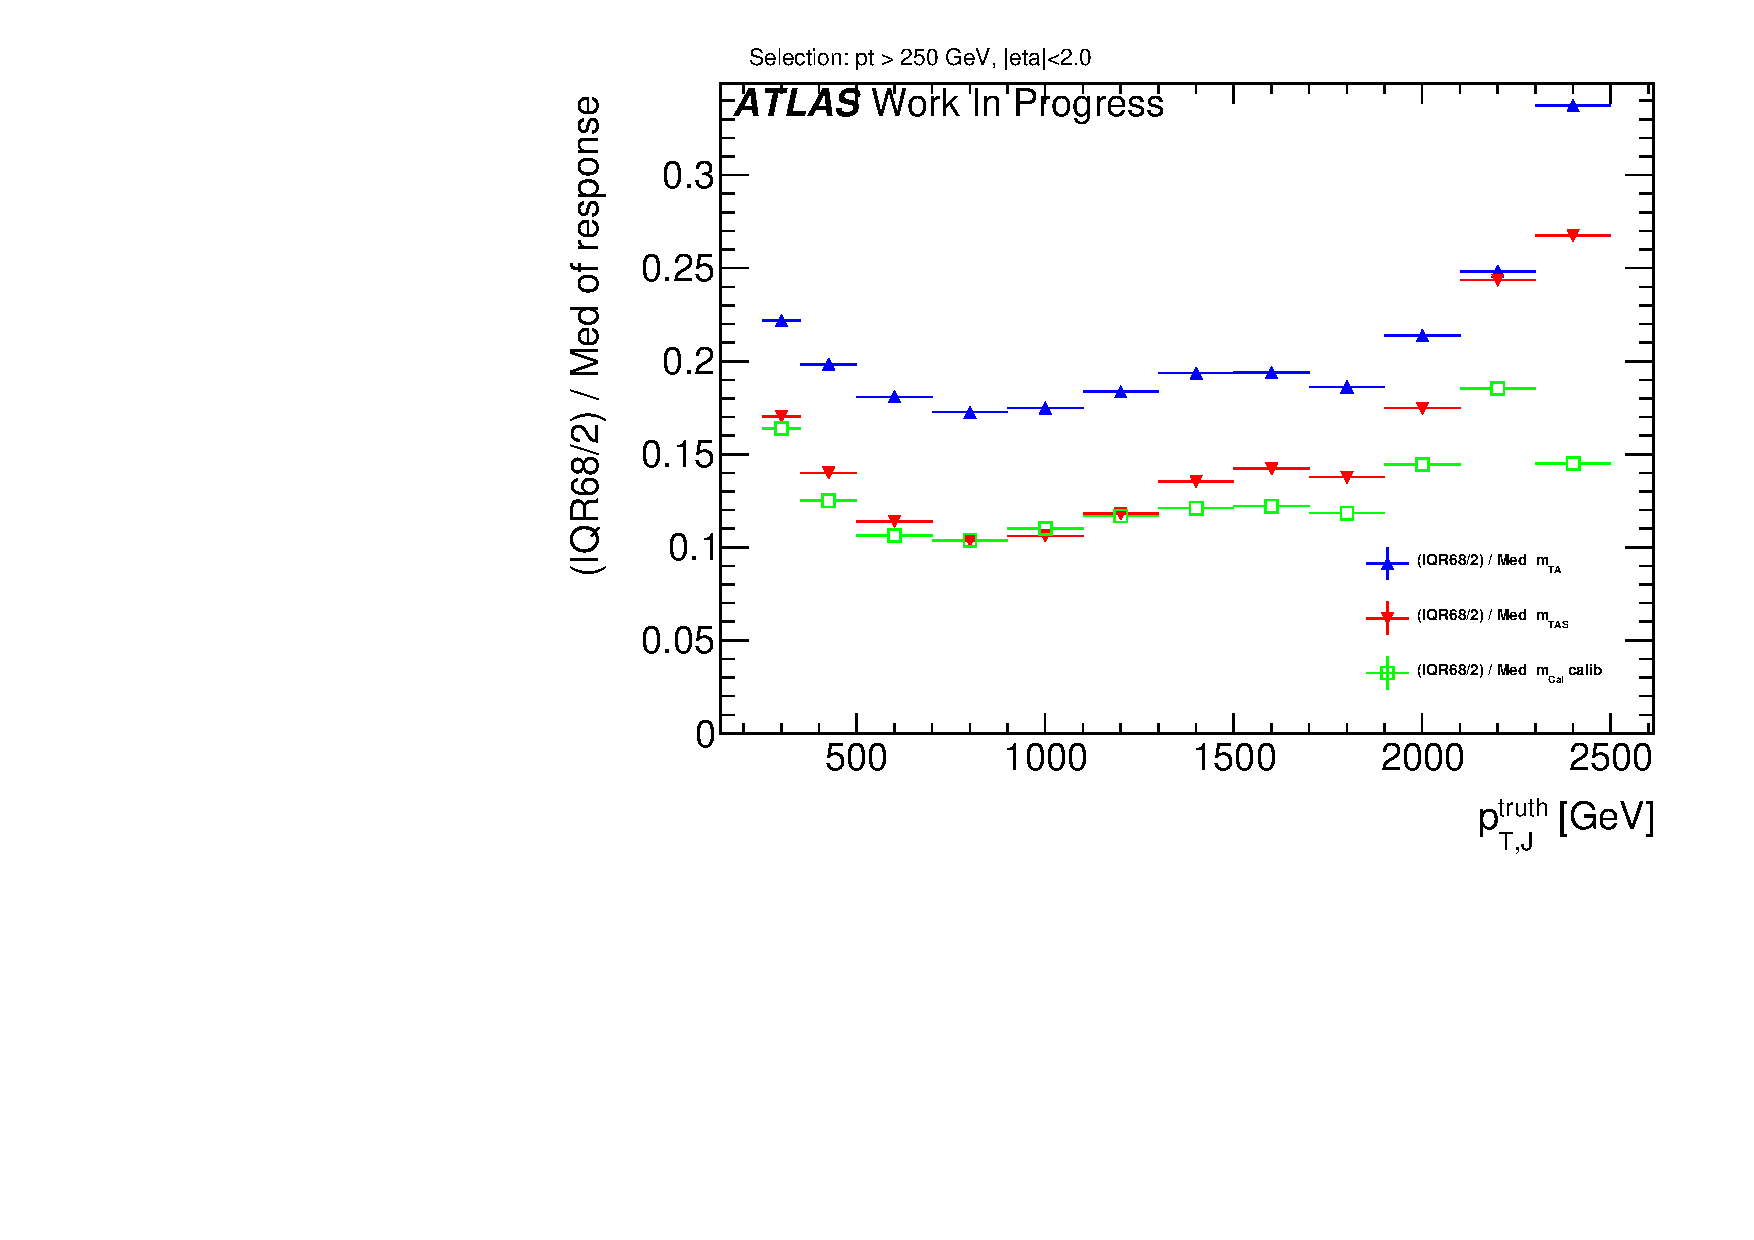
\includegraphics[width=0.7\textwidth]{jet_part/mtas/71graphcftr_h_JetRatio_mJ12CALOIQRoMHiggs.pdf}
%   \caption[$\mtas$ for boosted Higgs]{Performance of the $\mtas$ versus the $\mcal$ and $\mta$ for the boosted Higgs sample.}
%   \label{fig:mtas4}
% \end{figure}




\subsection{Performance in QCD Multijet Events}
The behavior of the QCD multijet sample is similar to the $W/Z$ sample, where the $\mta$ exhibits a crossing point in the middle-low regime $\pt\simeq900$ GeV and proceeds with a better performance at high transverse momenta.
Again the $\mtas$ follows this similarity showing no crossing point and an optimal overall behavior, both with respect to calorimeter- and track-assisted-based mass definition. On Figure \ref{fig:mtas5}.

\begin{figure}[!ht]
  \centering
%       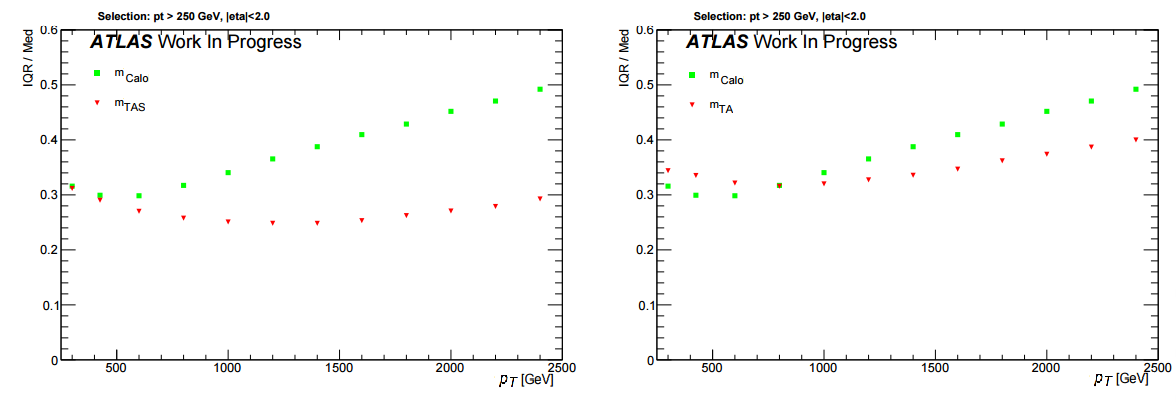
\includegraphics[width=\textwidth]{jet_part/mtas/qcdmtas.png}
        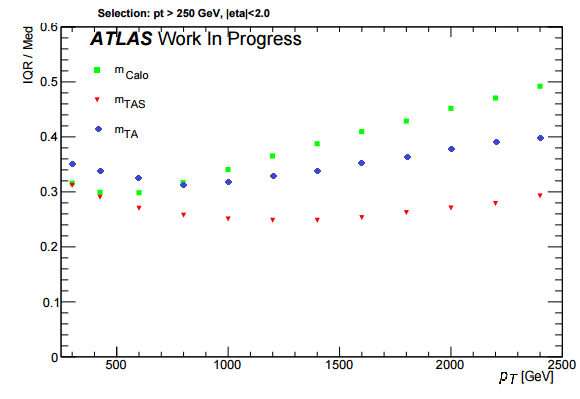
\includegraphics[width=0.50\textwidth]{jet_part/mtas/qcdmtastruffa.png}
   \caption[$\mtas$ for QCD jets]{Performance of the $\mtas$ versus the $\mcal$ and $\mta$ for the QCD multijet shows a much better behavior of the track-assisted sub-jet mass. Here shown $50\% \:\textrm{IQnR/median}$ and not the $\iqr$.}
  \label{fig:mtas5}
\end{figure}

\subsection{Performance in Massive $\tilde{W}\to q'\bar{q}$ Decays with $m_{\tilde{W}}=m_t$}
The massive $W$ sample is a special sample which was used to understand the behavior of top jets, whether its worse resolution was coming from the higher mass of the top quark or from the more complex decay topology (three-pronged instead of two-pronged decay and $b$-quark presence). 
The sample is almost identical to the $W/Z$ one ($W'\to WZ$) but in this case the SM electroweak boson have the mass of the top quark $m_{\tilde{W}}=m_t$.
In fact, from the rule $\Delta R=2m/p_T$, a bigger separation is expected between quarks from the hadronic decay.
The comparison with $\mcal$ is shown in Figure \ref{fig:mtas6}, together with the top-quark jet for completeness. As seen here, the performance of the latter is clearly worse than the former, the trend is yet very similar. This difference is interpreted in terms of different and more complex topology and hence higher sub-jet multiplicity: in the three sub-jet structure, resolving accurately the components is more challenging.

\begin{figure}[!ht]
  \centering
     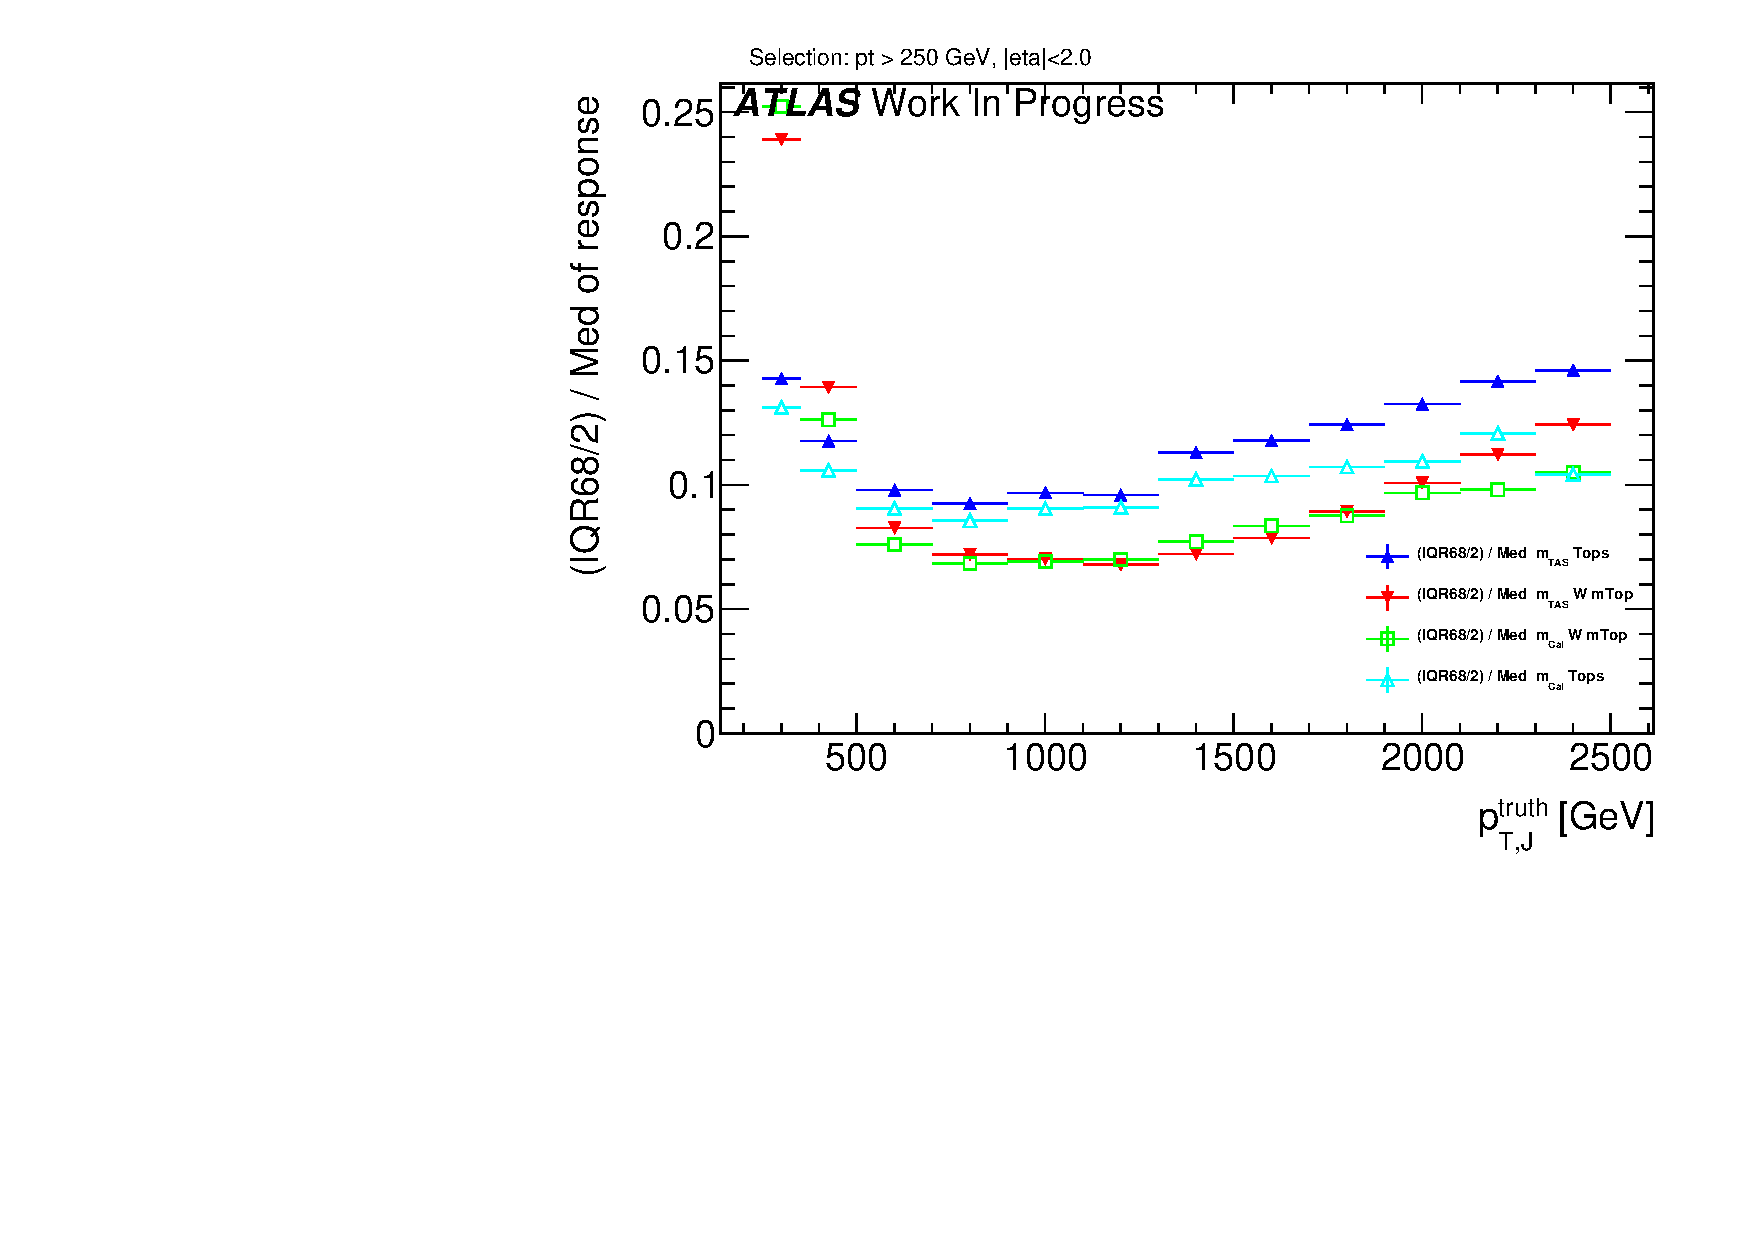
\includegraphics[width=0.55\textwidth]{jet_part/mtas/71graphcftr_h_JetRatio_mJ12CALOIQRoMcalib_WmassiveVsTops.pdf}
   \caption[$\mtas$ for massive $W/Z$]{Performance of the $\mtas$ versus the $\mcal$ for the massive $W/Z$ (in red and green); shown on the same plot also the top sample (in blue and light blue).}
  \label{fig:mtas6}
\end{figure}

\subsection{Stability of Mean of Response and Left-Hand-Side Integral }
The stability of the $\mtas$ was checked, although the IQnR is already a good quantifier of stability, explicitly for the mean of the mass response distribution and for the left-hand-side tail, as a function of the transverse momentum. This was an important check to assure the overall gaussianity of the final distribution in the whole spectrum of $\pt$, and suitability in regards of the calibration step, which is not discussed in this thesis.

The mean of the response distribution is shown for $W/Z$ decays in Figure \ref{fig:meanandtail}, left; as seen here, despite the mean being constantly below unity, its behavior is much more flat and independent of $\pt$, especially in the low-intermediate regime. This is surprising since the $\mcal$ is already shown after the calibration step, which is not taken instead for the $\mtas$. Conversely the left-hand-side tail of the mass response which is shown in the same figure, right, shows a more enhanced behavior than the $\mcal$, but still never reaches the 10\%. Of course an enhancement of the tail causes a loss of gaussianity and a number of jets which are reconstructed with a lower mass than they should, but it is still comparable with the calorimeter mass.

Those quantifiers show analogous behavior for the other samples considered and those figures can be found in the Appendix.

\begin{figure}
    \centering
    \begin{subfigure}[b]{0.45\textwidth}
	\centering
        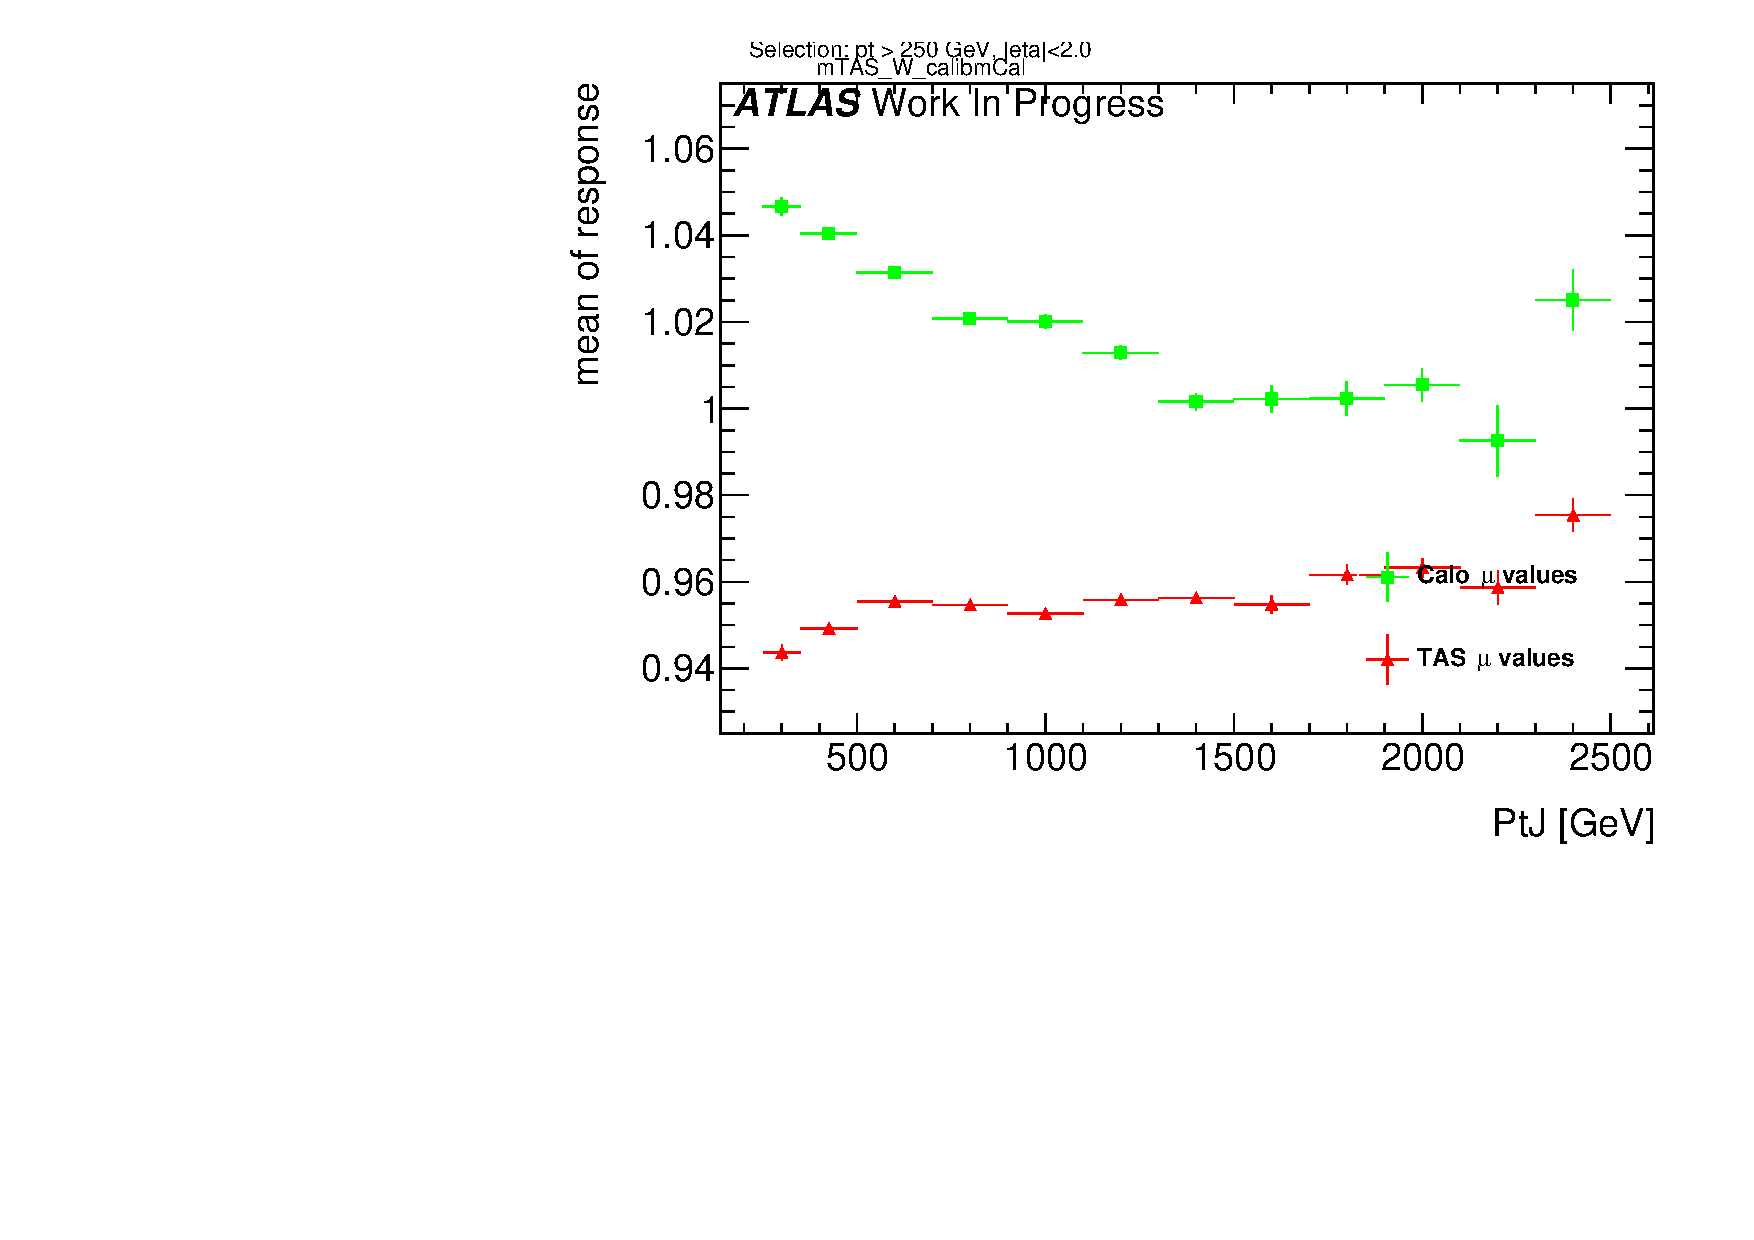
\includegraphics[width=\textwidth]{appendixB/mTAS_W_calibmCal_20:07:01-03-11-2016/71graph_h_JetRatio_mJ12CALO_meanResponseMvsTA.pdf}
%         \label{fig:tiger}
    \end{subfigure}
    \begin{subfigure}[b]{0.45\textwidth}
	\centering
        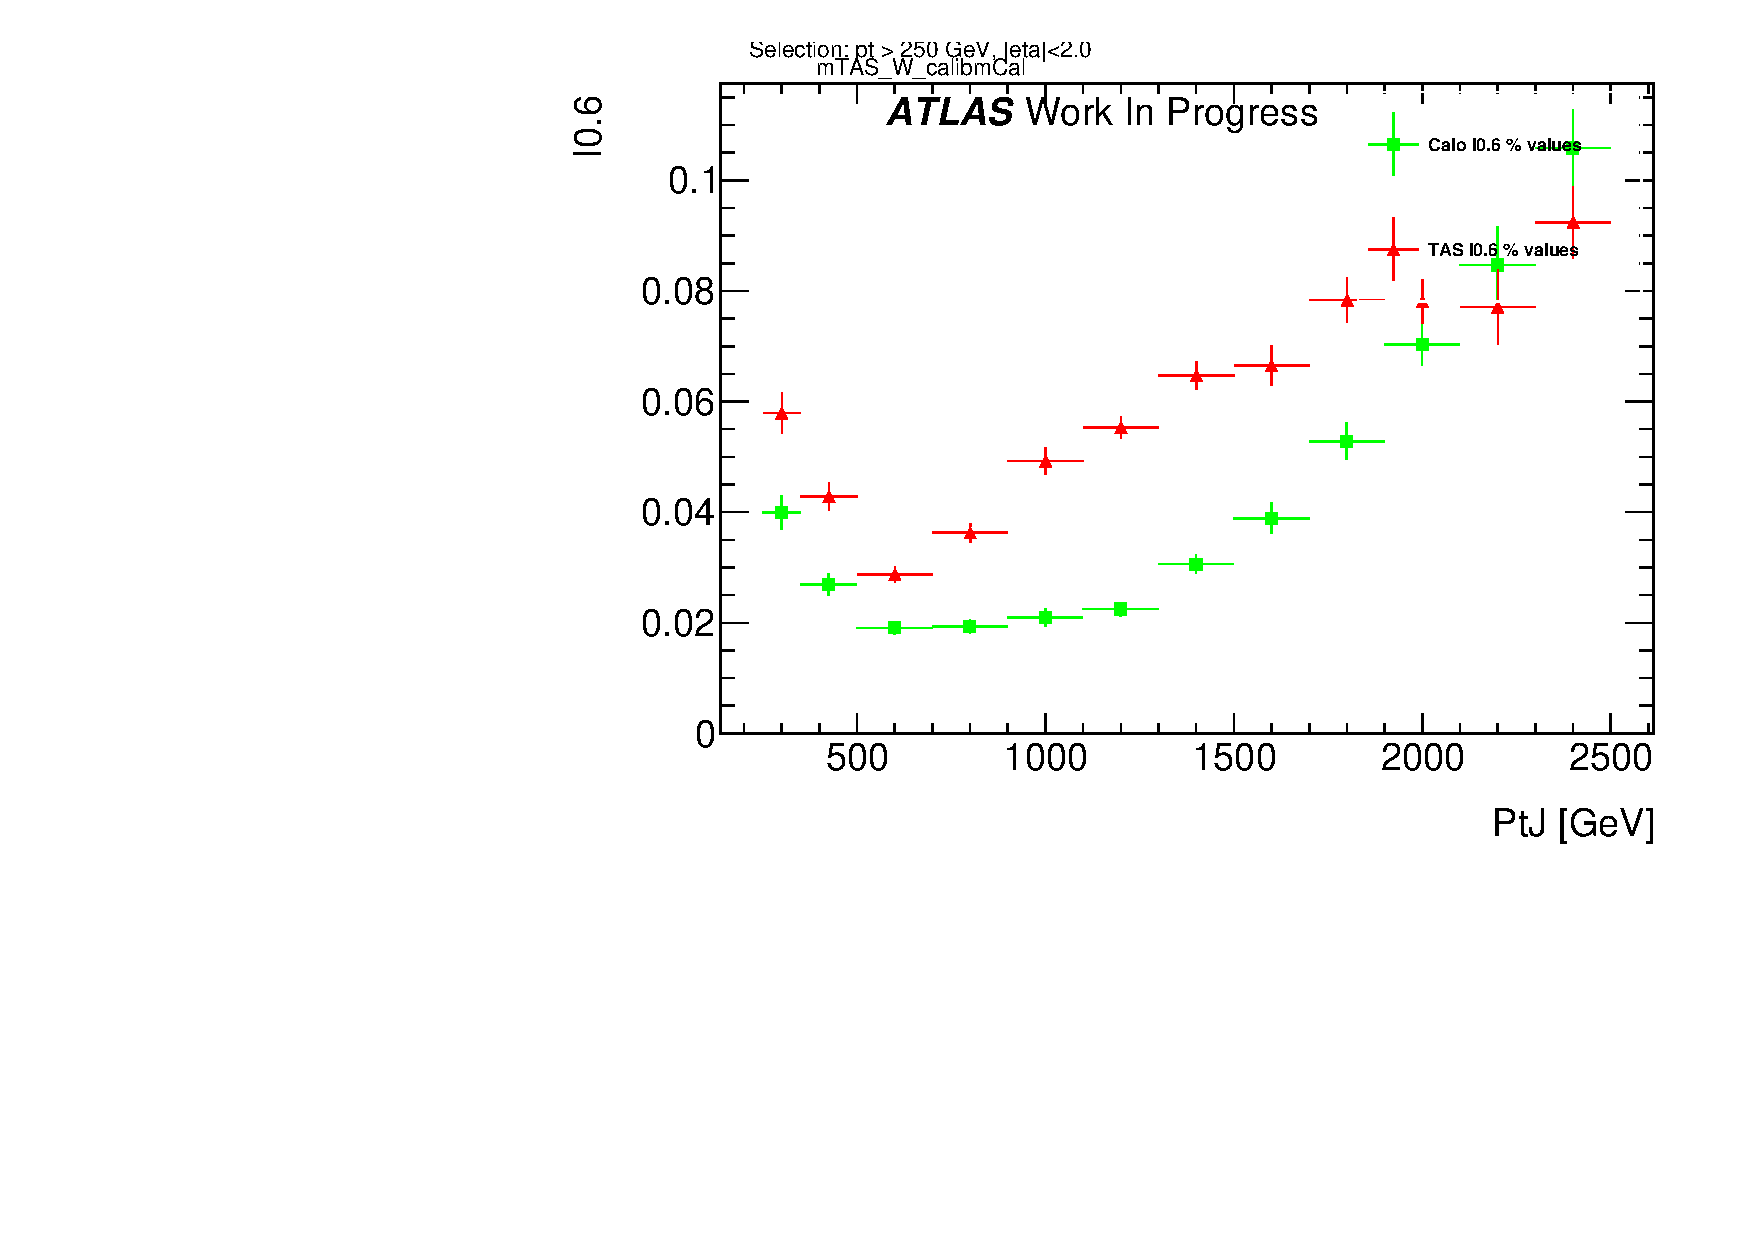
\includegraphics[width=\textwidth]{appendixB/mTAS_W_calibmCal_20:07:01-03-11-2016/74graph_h_JetRatio_mJ12CALO_I50ResponseMvsTAnorm.pdf}
 
%         \label{fig:gull}
    \end{subfigure}
    \caption[Mean and left-hand side integral for boosted $W/Z$]{Stability quantifiers which were checked for the $\mtas$: mean on the left and normalized left-hand side integral of the mass response distribution on the right. The mean is calculated from a Gaussian fit and the integral goes from 0 to 0.6.} 
    \label{fig:meanandtail}
\end{figure}

\subsection{Potential Improvements from Sub-jet Calibration}

An additional attempt of calibrating the sub-jet was also tried and, although the results were not substantially improved, it is presented in this section. This study was performed using only $W/Z$ samples.

% \subsection{Preliminary Studies on Sub-jet Calibration}
The \textit{perfect calibration} refers to the procedure of using $\mtas$ with truth-level information for calorimeter and tracker system, i.e. looking at the best possible scenario with an ideal detector. The performance is of course expected to be optimal, because of the use of the truth-level. This step was necessary as feasibility study, to understand whether ulterior efforts in this direction were meaningful.
% The first attempt in calibrating the sub-jets had as start a ``perfect calibration'', which means using the truth-level information from the MC sample \textit{before} the interaction with the calorimeter.
Truth-level tracks are the particles in the jet which have an electric charge and are stable, truth-level sub-jets are all the particles, charged and not, which are ghost associated to the calorimeter sub-jets.
There are few possibilities in doing so, here some nomenclature for this study will be introduced:
\begin{itemize}
 \item $\mtas$ using truth-level sub-jets and tracks; normal tracks (with all detector effects) are used to assist the truth-level sub-jets;
 \item $\mtas$ using truth-level tracks and truth-level sub-jets; the truth-level tracks are used to assist the truth-level sub-jets;
 \item $\mcal$ truth, calculated using only the truth sub-jets.
\end{itemize}


% \subsubsection{Perfect Calibration}


% \begin{figure}[!ht]
%   \centering
%       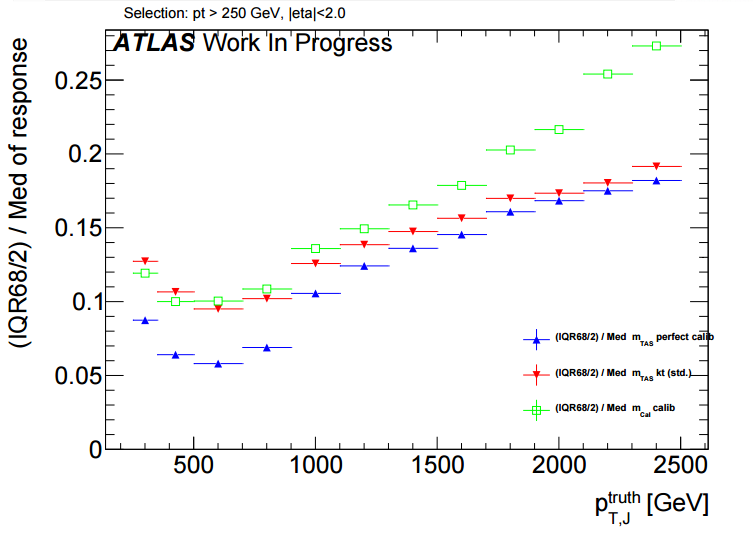
\includegraphics[width=0.7\textwidth]{jet_part/calib/perfcalib.png}
%   \caption[Perfect calibration]{Performance of the perfect calibration, using truth-level sub-jets and truth-level tracks. It shows room for improvement especially at low-middle $\pt$.}
%   \label{fig:perfcalib}
% \end{figure}


\subsubsection{Simple Sub-jet Calibration}
The perfect calibration using truth level sub-jets and tracks is shown in Figure \ref{fig:perfcalib4} in blue dots; since the performance exhibits room for big improvement below $\sim$ 1 TeV and moderate to small improvement above this value, the second step of a simple calibration was tried.

Following the example of calibration of jets in general, a simple approach to emulate this procedure was tried, constructing in various bins of transverse momenta the responses of the sub-jet's energy to derive the weights factors to be applied. The detailed procedure is as follows:
\begin{enumerate}
 \item Responses in energy $R_E=E^{reco}/E^{truth}$ were built in several bins of $\pt$, spanning to the whole transverse momentum range;
 \item The mean $\mu_R$ of this response was calculated via a fit to the Gaussian core;
 \item Those values (\textit{scale factors}) were stored and applied again to the sub-jets before the computation of the $\mtas$ via 4-momentum correction $E'=E/\mu_R$; the $\pt$ (the value which only enters the $\mtas$ variable) was changed then correspondingly to keep the sub-jet's mass constant.
\end{enumerate}

This procedure was called \textit{poor man's calibration} or PM calibration or \textit{simple calibration}.
A check on the $\pt$ response before and after calibration together with the mean of the entire Large-$R$ jet response is shown in Figure \ref{fig:calibA} and \ref{fig:calibA2} in Appendix.

The results are on Figure \ref{fig:perfcalib4}; there are only marginal improvements in few ranges of low transverse momentum where the scale factors are further away from unity, and the overall observable is not performing better than the standard $\mtas$. This is interpreted both in terms of a missing calibration as a function of the $\eta$ variables (having hence a befit from the crack region) and because the correction done on average does not provide the sufficient handle in a jet-by-jet basis, especially when all the sub-jets are rescaled by similar factors (which translates into a similarity of $\pt$s of the sub-jets, often the case for e.g. $W/Z$ decays, less for tops jets entirely contained in the large-$R$ jet).

\begin{figure}[!ht]
  \centering
      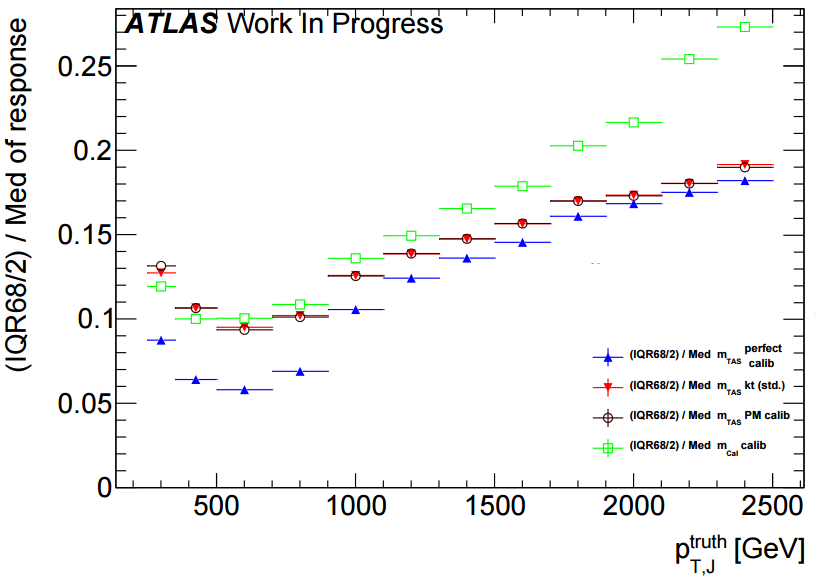
\includegraphics[width=0.55\textwidth]{jet_part/calib/perfectcalib4.png}
  \caption[Simple calibration]{Performance of the poor man's calibration. The improvement is marginal throughout the entire transverse momentum space.}
  \label{fig:perfcalib4}
\end{figure}

\subsection{Limitation of $\mtas$ from tracking}
The final effort to understand the various and competing effects, which take place in the $\mtas$ and which was inspired by the perfect calibration procedure, brought to a final study on the variable to understand the reason for the worsening of the resolution at high transverse momenta, using again the truth MC information.

The preliminary investigation in this direction was then the study on the track mass resolution: a response of the mass of the tracks associated to the jet ($m^{track}$), was constructed, using the truth-level tracks.

The result is shown on Figure \ref{fig:trackdegrade}: for the samples considered, it shows a linear degradation of the mass of the tracks associated to the jet ($m^{track}$), both for massive and SM $W/Z$.

\begin{figure}[!ht]
  \centering
      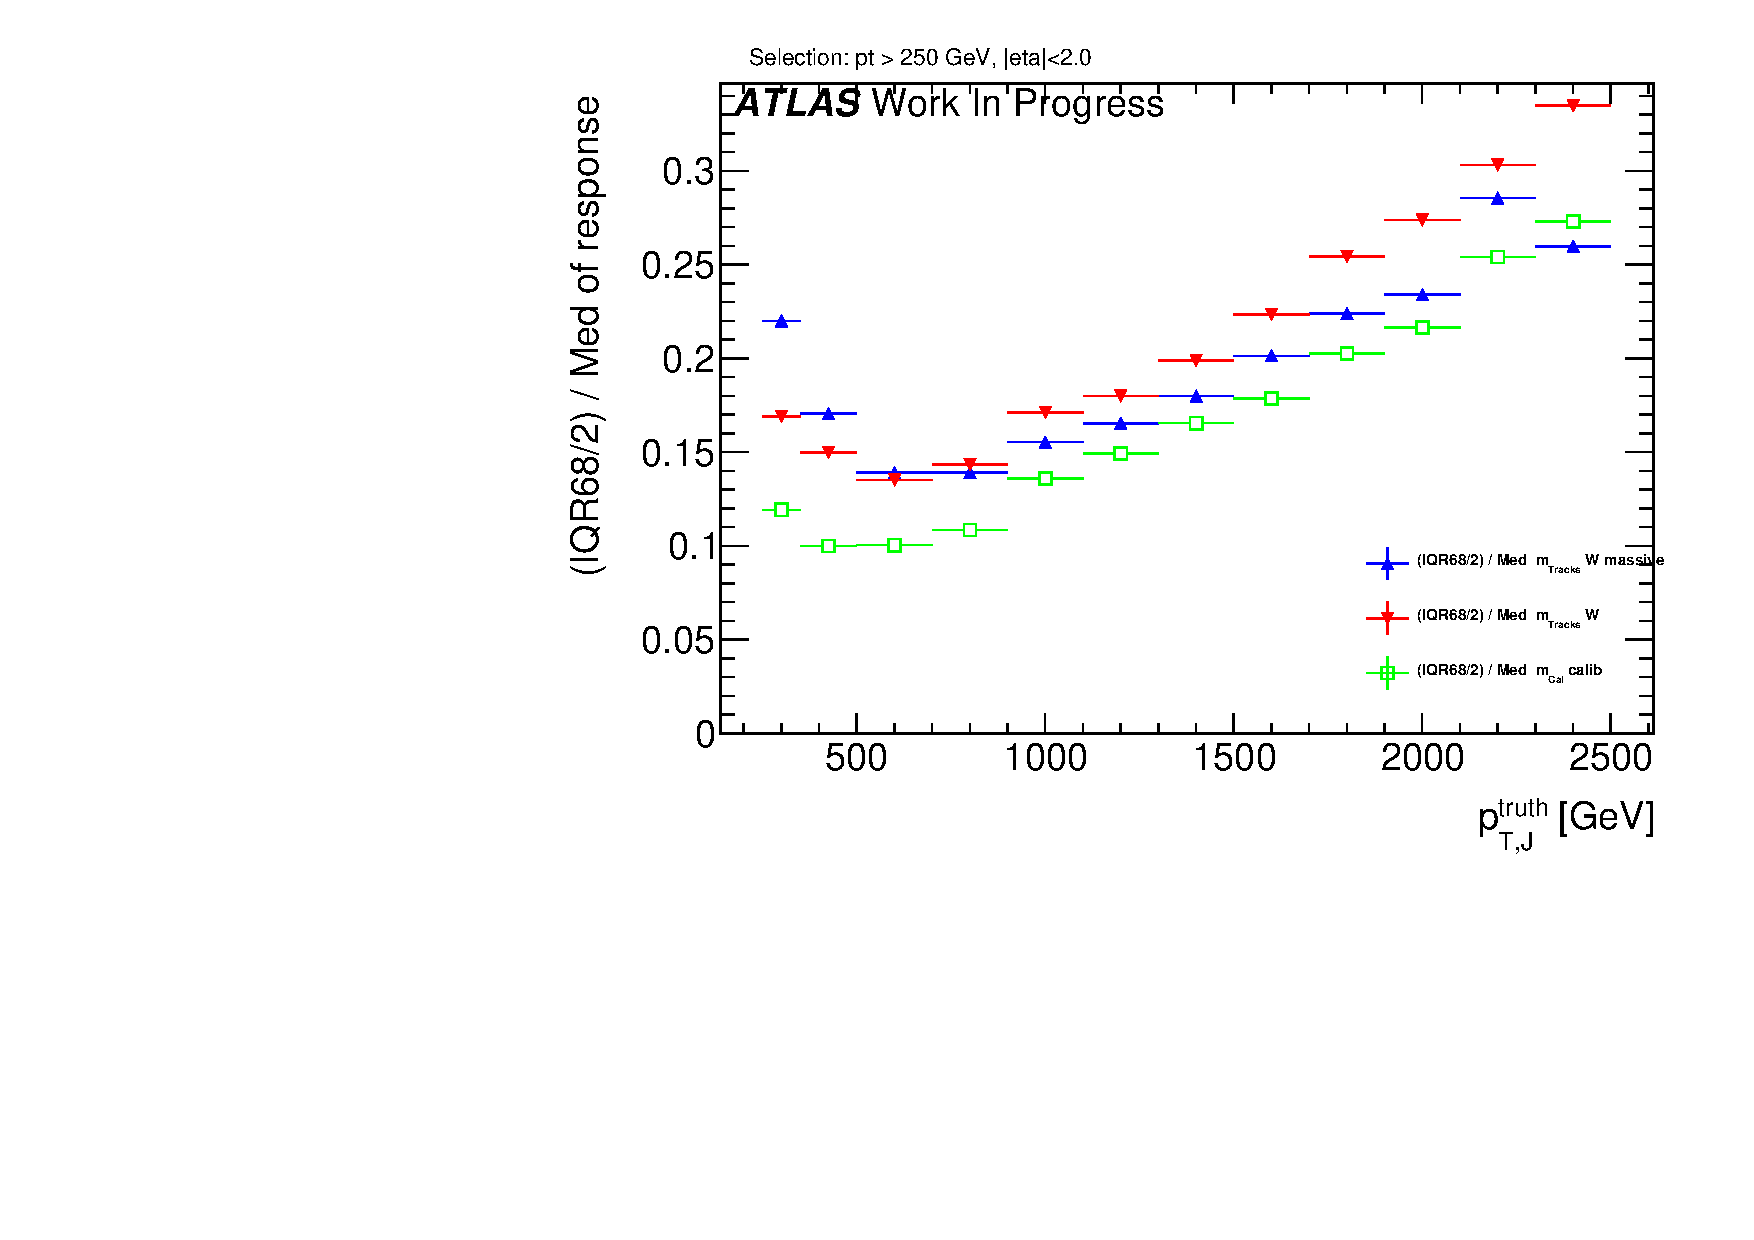
\includegraphics[width=0.55\textwidth]{jet_part/calib/71graphcftr_h_JetRatio_mJ12CALOIQRoMcalib_trkmass.pdf}
  \caption[Track mass degradation in tops and massive $W/Z$]{The performance of the track mass ($m^{track}$) in blue and red for massive $W$ sample and boosted $W/Z$ respectively; for reference in green the calorimeter mass of the large-$R$ jet.}
  \label{fig:trackdegrade}
\end{figure}
% ***change figures with the one in appendix***
The hypothesis of the degradation of the $\mtas$ driven by the tracks is also supported by the Figure \ref{fig:breakdown1} in Appendix, where the truth-level tracks are used instead of real tracks to compute the variable; it can be seen the flat behavior at high $\pt$, hence ascribing the worsening of the resolution to tracks at higher transverse momenta.

A complete breakdown of the variable in terms of truth-level particles is given in Figure \ref{fig:breakdown2}, where all the different components are separated.
In particular the black dots show the $\mtas$ using truth-level sub-jets but real tracks for the track assistance procedure.
Even combining this truth-level information, in fact, it shows a large worsening of the performance (truth-level sub-jets only are shown as blue dots).
On the other side using again truth-level tracks for the track assistance procedure of the truth-level sub-jet, shows a recovery of the loss in performance.

% Particularly interesting is the black dots, which 
% uses truth-level sub-jet but real tracks, which worsen the overall performance of the truth-level sub-jet alone (shown in light blue dots).

% \begin{figure}[!ht]
%   \centering
%       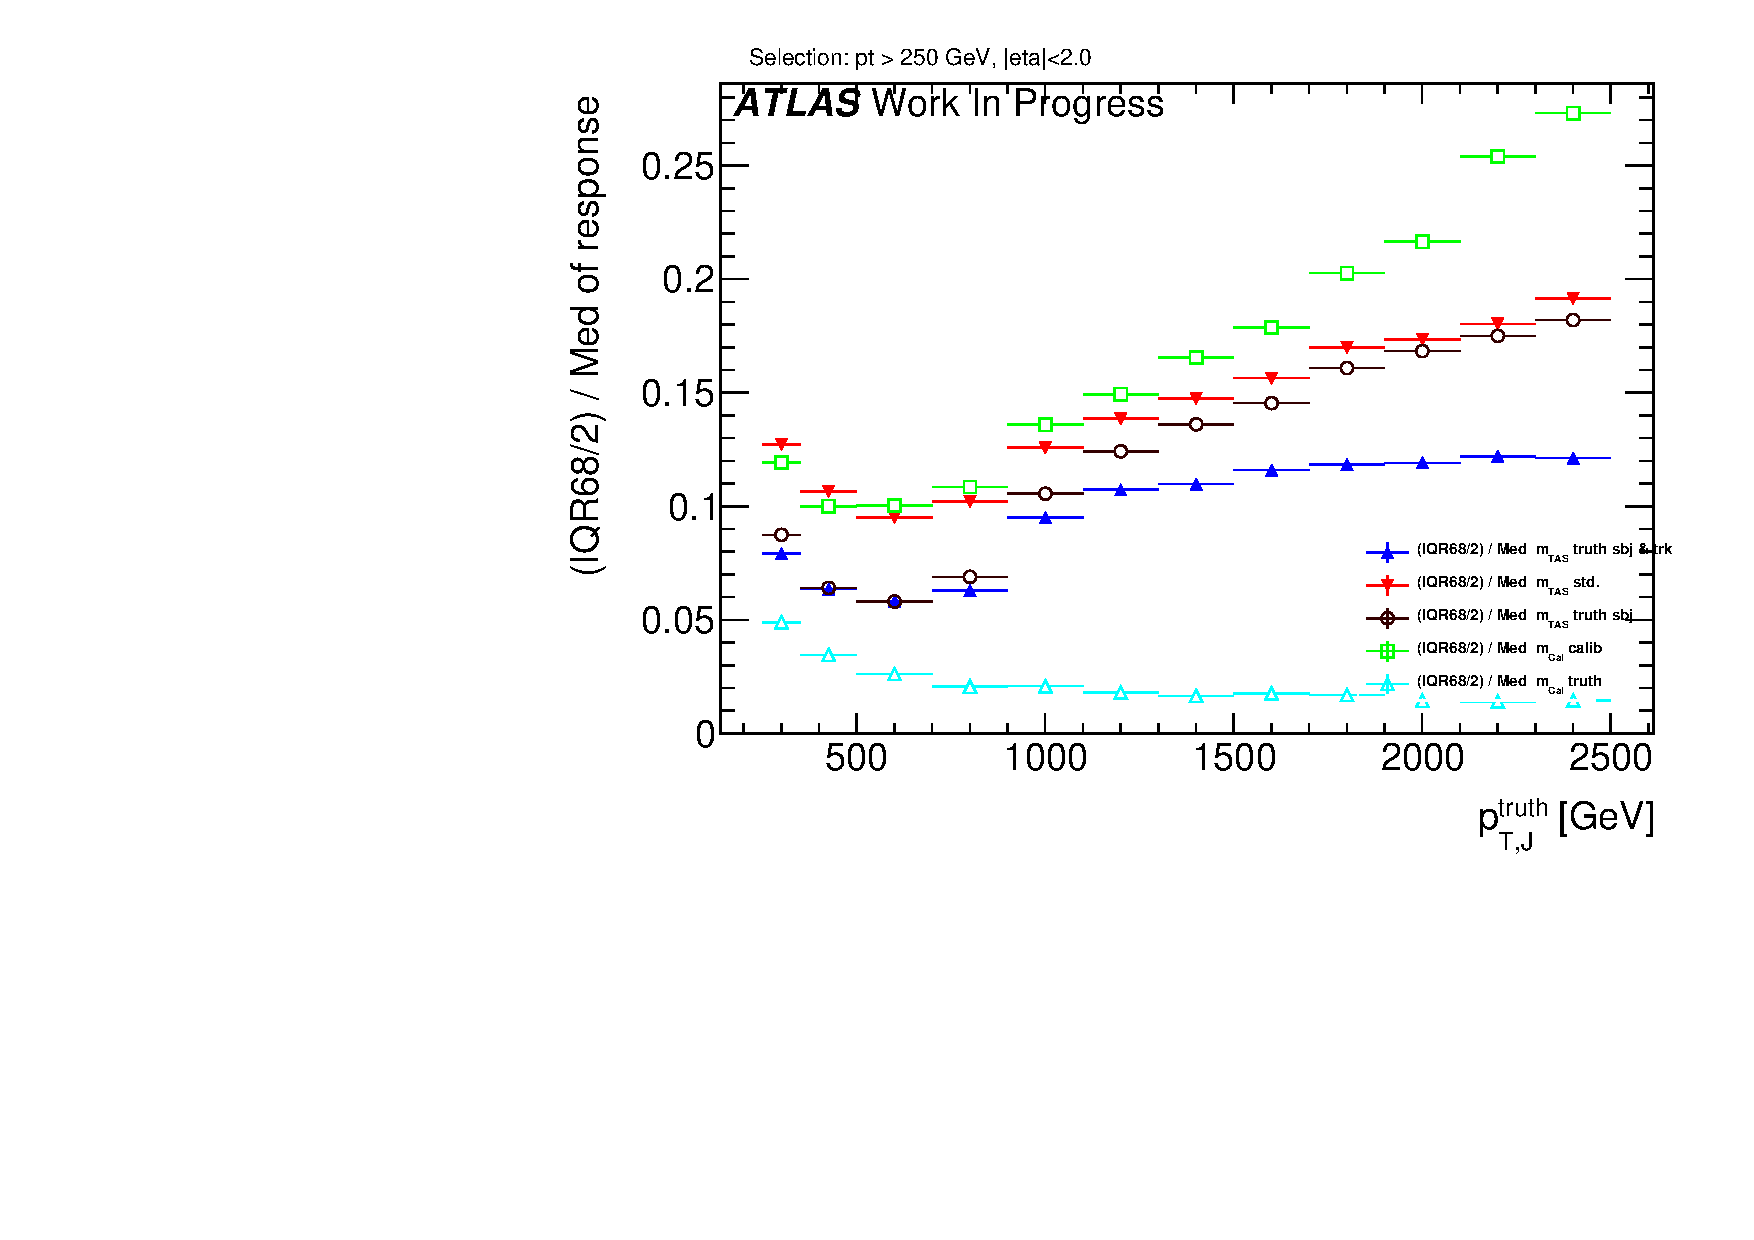
\includegraphics[width=0.7\textwidth]{jet_part/calib/71graphcftr_h_JetRatio_mJ12CALOIQRoM4Truths.pdf}
%   \caption[Breakdown of the $\mtas$ ]{Breakdown of the $\mtas$ in its component using truth-level information for boosted $W/Z$ decays. In blue the $\mtas$ using truth-level sub-jets and truth level tracks, in black $\mtas$ using truth level sub-jets but real tracks and in light blue for reference the mass of the truth level particles associated to the sub-jets. As usual, in red and green the standard $\mtas$ and the $\mcal$}
%   \label{fig:breakdown2}
% \end{figure}

% Other results using truth-level information on boosted tops are shown and described in the Appendix.

\begin{figure}
    \centering
    \begin{subfigure}[b]{0.45\textwidth}
  \centering
      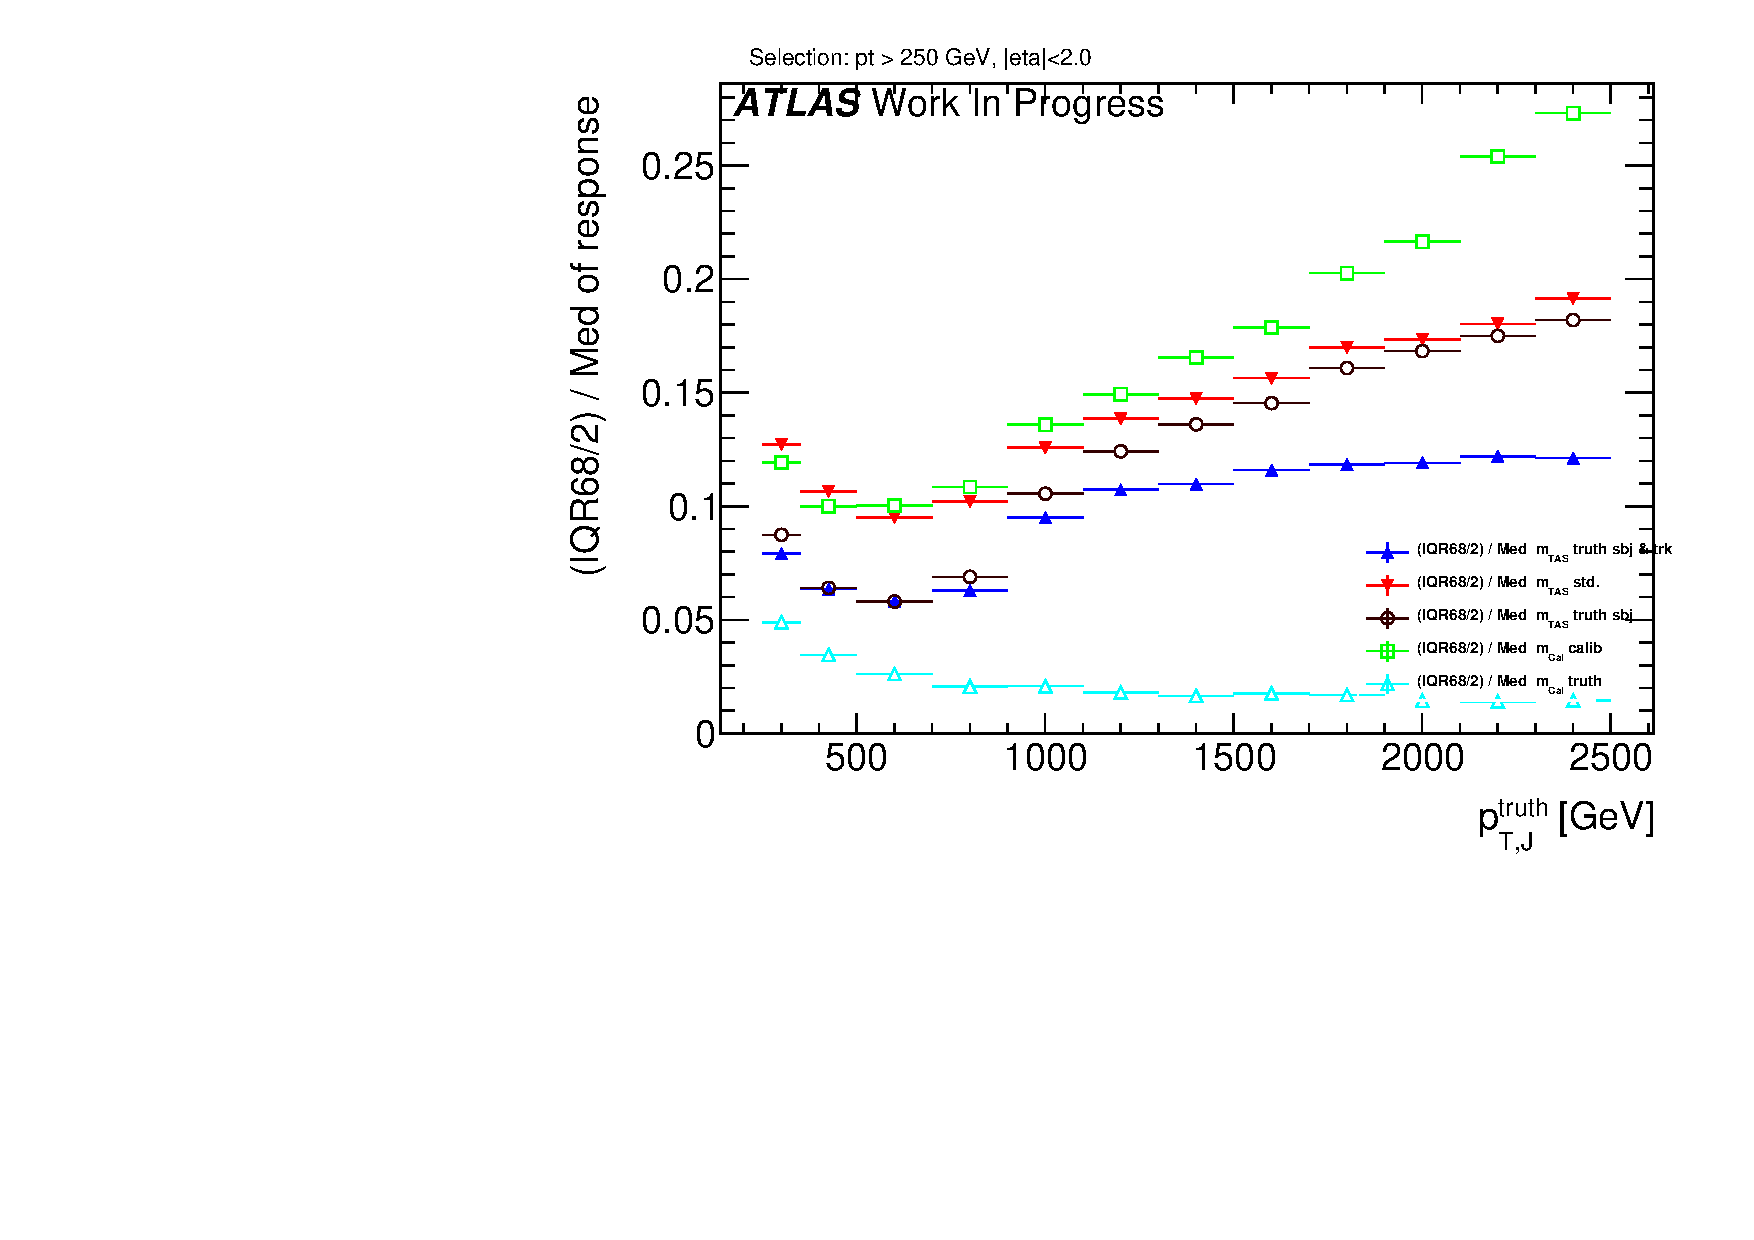
\includegraphics[width=0.9\textwidth]{jet_part/calib/71graphcftr_h_JetRatio_mJ12CALOIQRoM4Truths.pdf}
  \caption[Breakdown of the $\mtas$ ]{$W/Z$ jets}
  \label{fig:breakdown2}
    \end{subfigure}
    \begin{subfigure}[b]{0.45\textwidth}
  \centering
      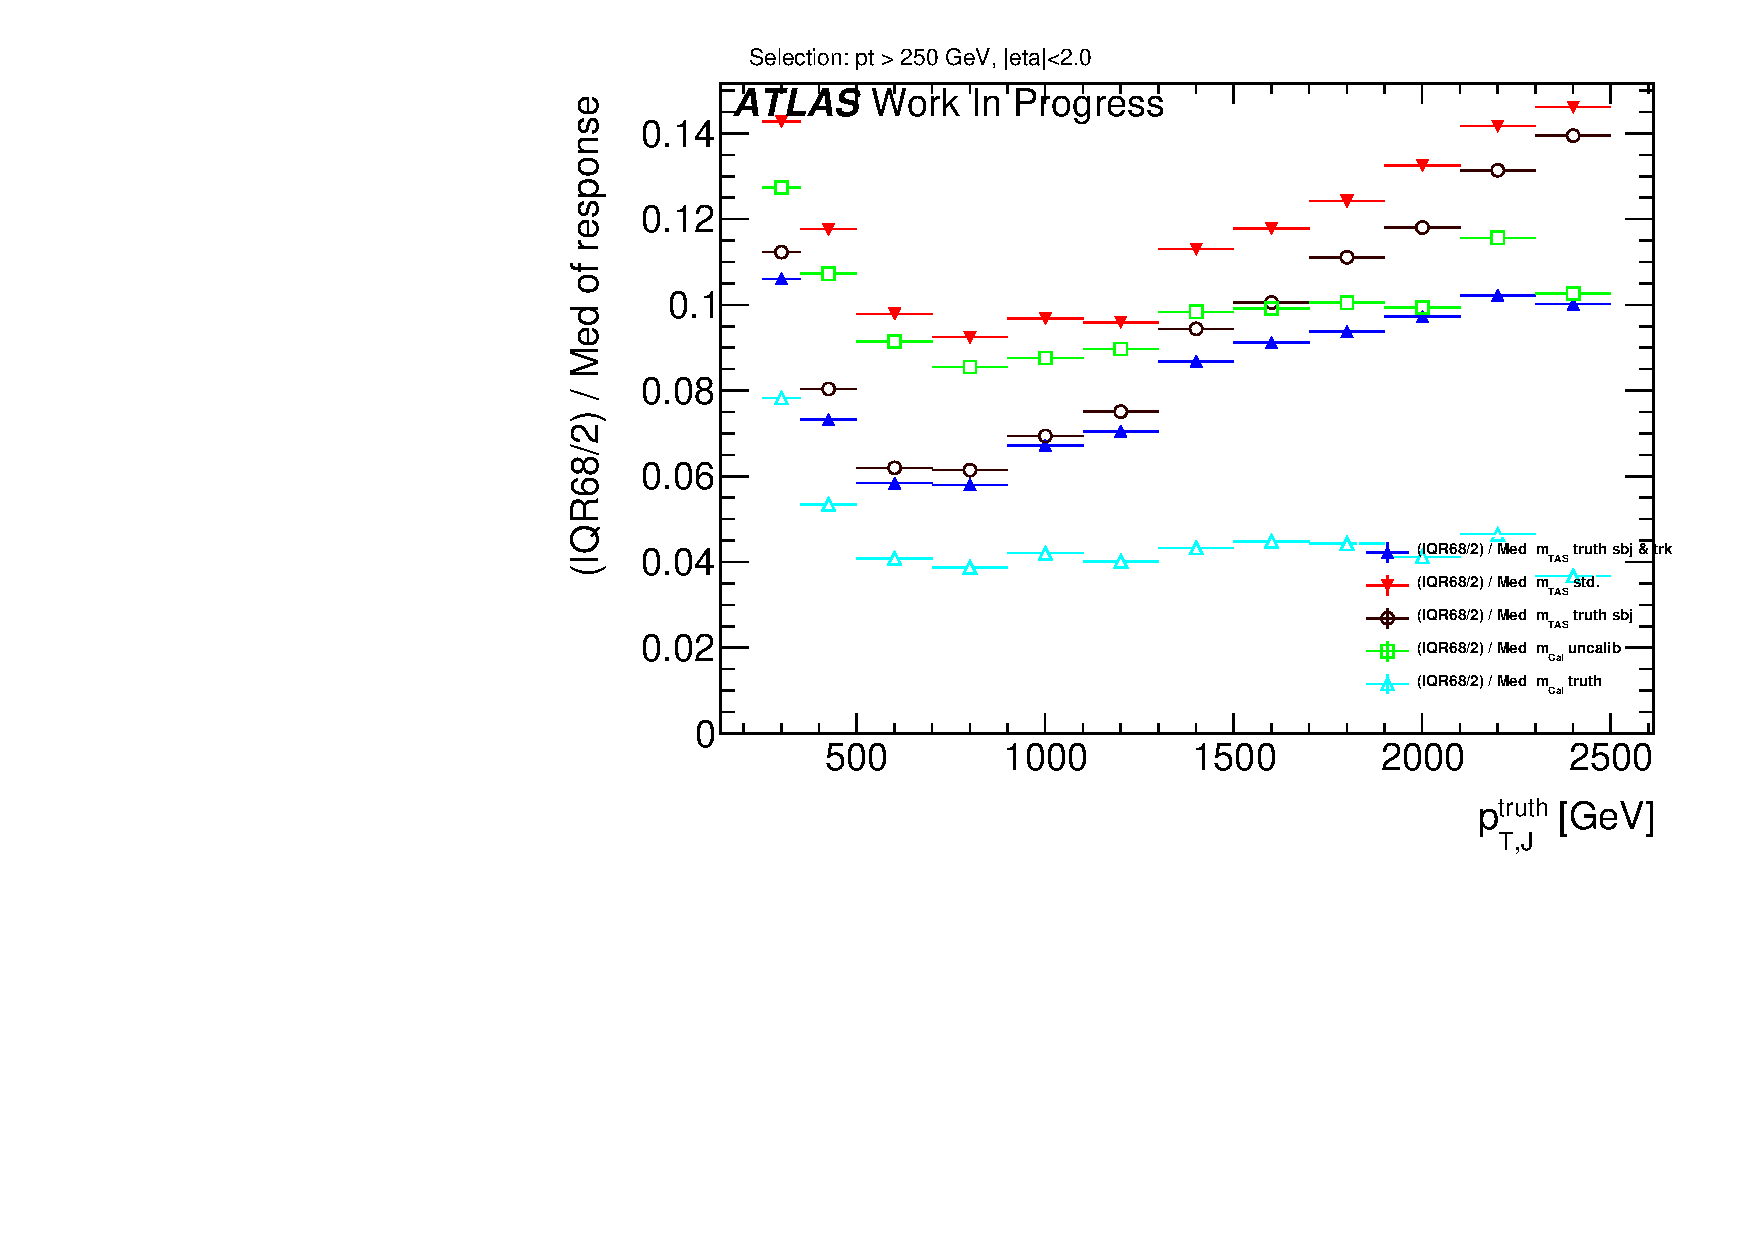
\includegraphics[width=0.9\textwidth]{jet_part/appendixA/71graphcftr_h_JetRatio_mJ12CALOIQRoM4TruthsTops.pdf}
  \caption[Breakdown of the $\mtas$ ]{top jets}
  \label{fig:breakdown3}
 
    \end{subfigure}
    \caption[Breakdown of the $\mtas$]{Breakdown of the $\mtas$ in its component using truth-level information for $W/Z$ decays, on the left. In blue the $\mtas$ using truth-level sub-jets and truth level tracks, in black $\mtas$ using truth level sub-jets but real tracks and in light blue for reference the mass of the truth level particles associated to the sub-jets. As usual, in red and green the standard $\mtas$ and the $\mcal$. On the right the same for top jets.} 
    % \label{fig:meanandtail}
\end{figure}

% \chapter{Limitation of the $\mtas$}
Additional studies on the limitation of the $\mtas$ based on MC studies without detector interactions are also presented. In particular, the truth study presented for $W/Z$ decay in were extended for top quark decays.

As seen on Figure \ref{fig:breakdown3}, the breakdown of the $\mtas$ shows that, in particular for the high transverse momenta regimes, the tracks are subjected to fast degradation which makes their combination with the calorimeter mass not anymore an advantage. 

This is a limitation which was expected and understood from the detector performance point of view, and here shows the impossibility, with the variables which are presented here $\mta$ and $\mtas$ to reach a competitive standpoint with the $\mcal$ in the extreme kinematic regime for the top quark decay.

In black, in fact, the performance of the $\mtas$ variable using tracks with detector effect and sub-jets without those effects, shows this intrinsic limit which takes place already at 1.5 TeV.

The crossing point is, as already pointed out for the top jets, present because of the optimal performance of the calorimeter system caused by the higher mass of the top quark, and partially also because of its more complex decay structure and difficulty to be resolved in sub-jets.

% \begin{figure}[!ht]
%   \centering
%       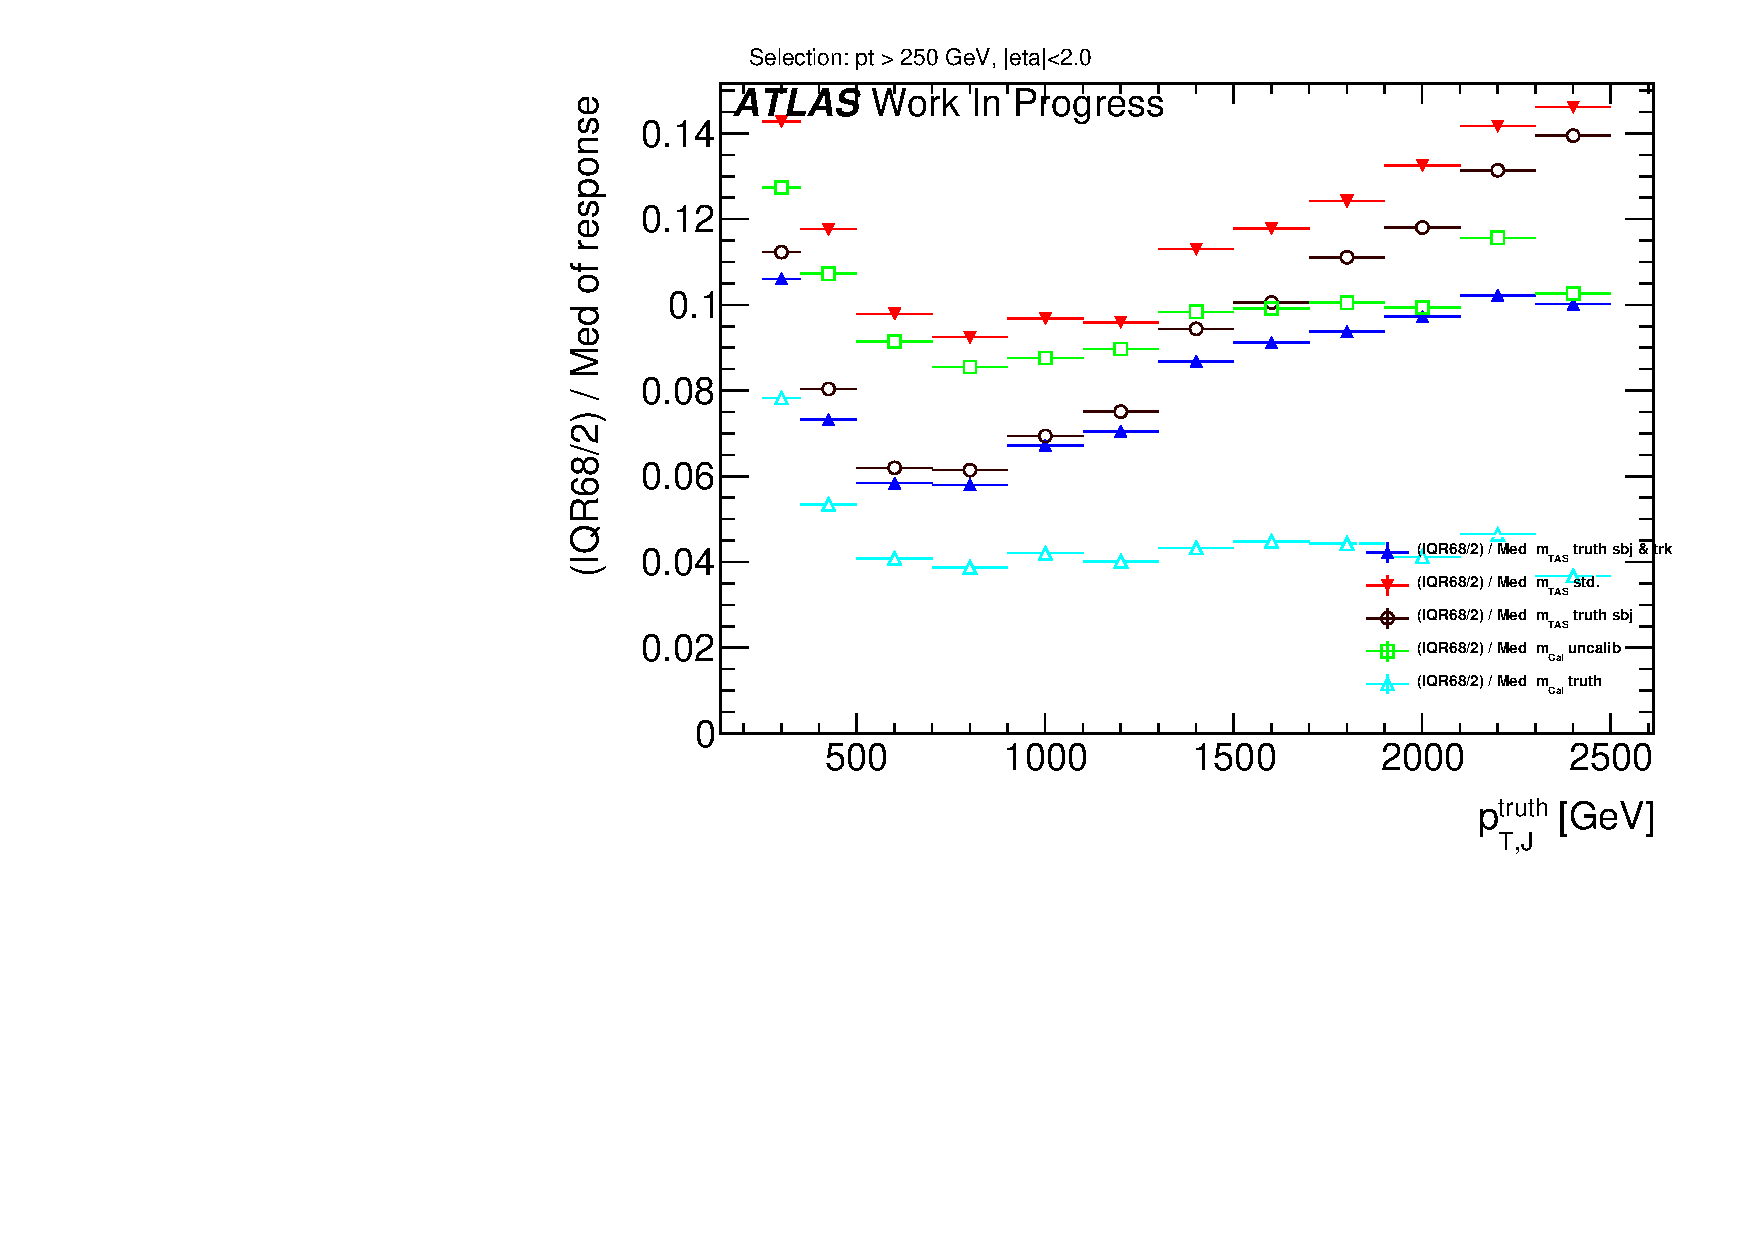
\includegraphics[width=0.7\textwidth]{jet_part/appendixA/71graphcftr_h_JetRatio_mJ12CALOIQRoM4TruthsTops.pdf}
%   \caption[Breakdown of the $\mtas$ ]{Breakdown of the $\mtas$ in its component using truth-level information for boosted top quarks decays.}
%   \label{fig:breakdown3}
% \end{figure}



% \subsection{Large-R jet: Calibration}
% The jet mass scale calibration aims to correct the reconstructed jet mass to the particle-level jet mass by applying calibration factors derived from a sample of simulated QCD multijet events, with an analogous procedure described in \ref{sec:calib} for the jet energy scale.
% 
% \subsection{Large-R jet: Uncertainties}


\subsection{Performance with Alternate Inputs to the $\mtas$}
\label{sec:alternate}

There are quite a few ways to modify the track-assisted sub-jet mass; however, all the alternative approaches showed worse performance, and they are mentioned here for completeness only.
The per-track four momentum correction scheme which is used for the ECF and the n-Subjettiness and also explored with the $\mtas$ with no significant difference was described in \ref{sec:tas}.

The other alternatives considered were: 
\begin{itemize}
 \item for the tracks:
 \begin{itemize}
   \item use of tracks not as input directly, but only taking those belonging to anti-k$_t$ reclustered track-jet with radius of 0.3 or 0.2;
   \item tighter or looser quality conditions were explored;
   \item tighter or looser primary vertex association requirement were explored.
 \end{itemize}
 \item for the sub-jets:
  \begin{itemize}
   \item the trimming procedure was modified: various radii $R_{sub}$ of the sub-jets were tested;
   \item the sub-jets were reclustered using not only the standard k$_t$, but also anti-k$_t$ and C/A.
  \end{itemize}
  \item for the procedure: different 4-momentum correction scheme was also studied in more details, see \ref{sec:tas}.
\end{itemize}

The different reclustering algorithm choice has a deep impact and was studied in details, since it changes the topo-cluster added to the sub-jets and the tracks associated to them. The situation is depicted in the event-display in Figure \ref{fig:evtdspl}; the display on the left shows the standard choice of k$_t$, the one on the right shows the modified approach anti-k$_t$. 

In Figure \ref{fig:allalgow} \ref{fig:allalgotop} \ref{fig:allalgohiggs} the performance for $W/Z$, tops and Higgs jets are shown, respectively. It can be seen that the k$_t$ algorithm provides the best observable definition, in all the samples considered. However, the anti-k$_t$ algorithm provides similar performances; this was an important check as the jet calibration procedure currently going on in ATLAS, the \textit{R-Scan} procedures includes the anti-k$_t$ algorithm with radius of R=0.2 and aims at providing the calibration and uncertainties that could be used directly in the computation of the $\mtas$.
% *** quantify the difference ***

\begin{figure}[!ht]
  \centering
      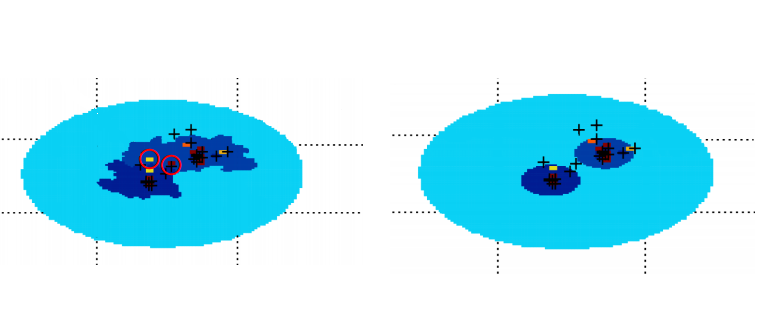
\includegraphics[width=0.55\textwidth]{jet_part/mtas/evtdspl.png}
  \caption[Different reclustering in event display]{An example of event-display shows the differences in the reclustering algorithm used for the sub-jets: on the right  k$_t$ and on the left anti-k$_t$. Highlighted some constituents trimmed away with the second choice.}
  \label{fig:evtdspl}
\end{figure}



% \begin{figure}
%     \centering
%    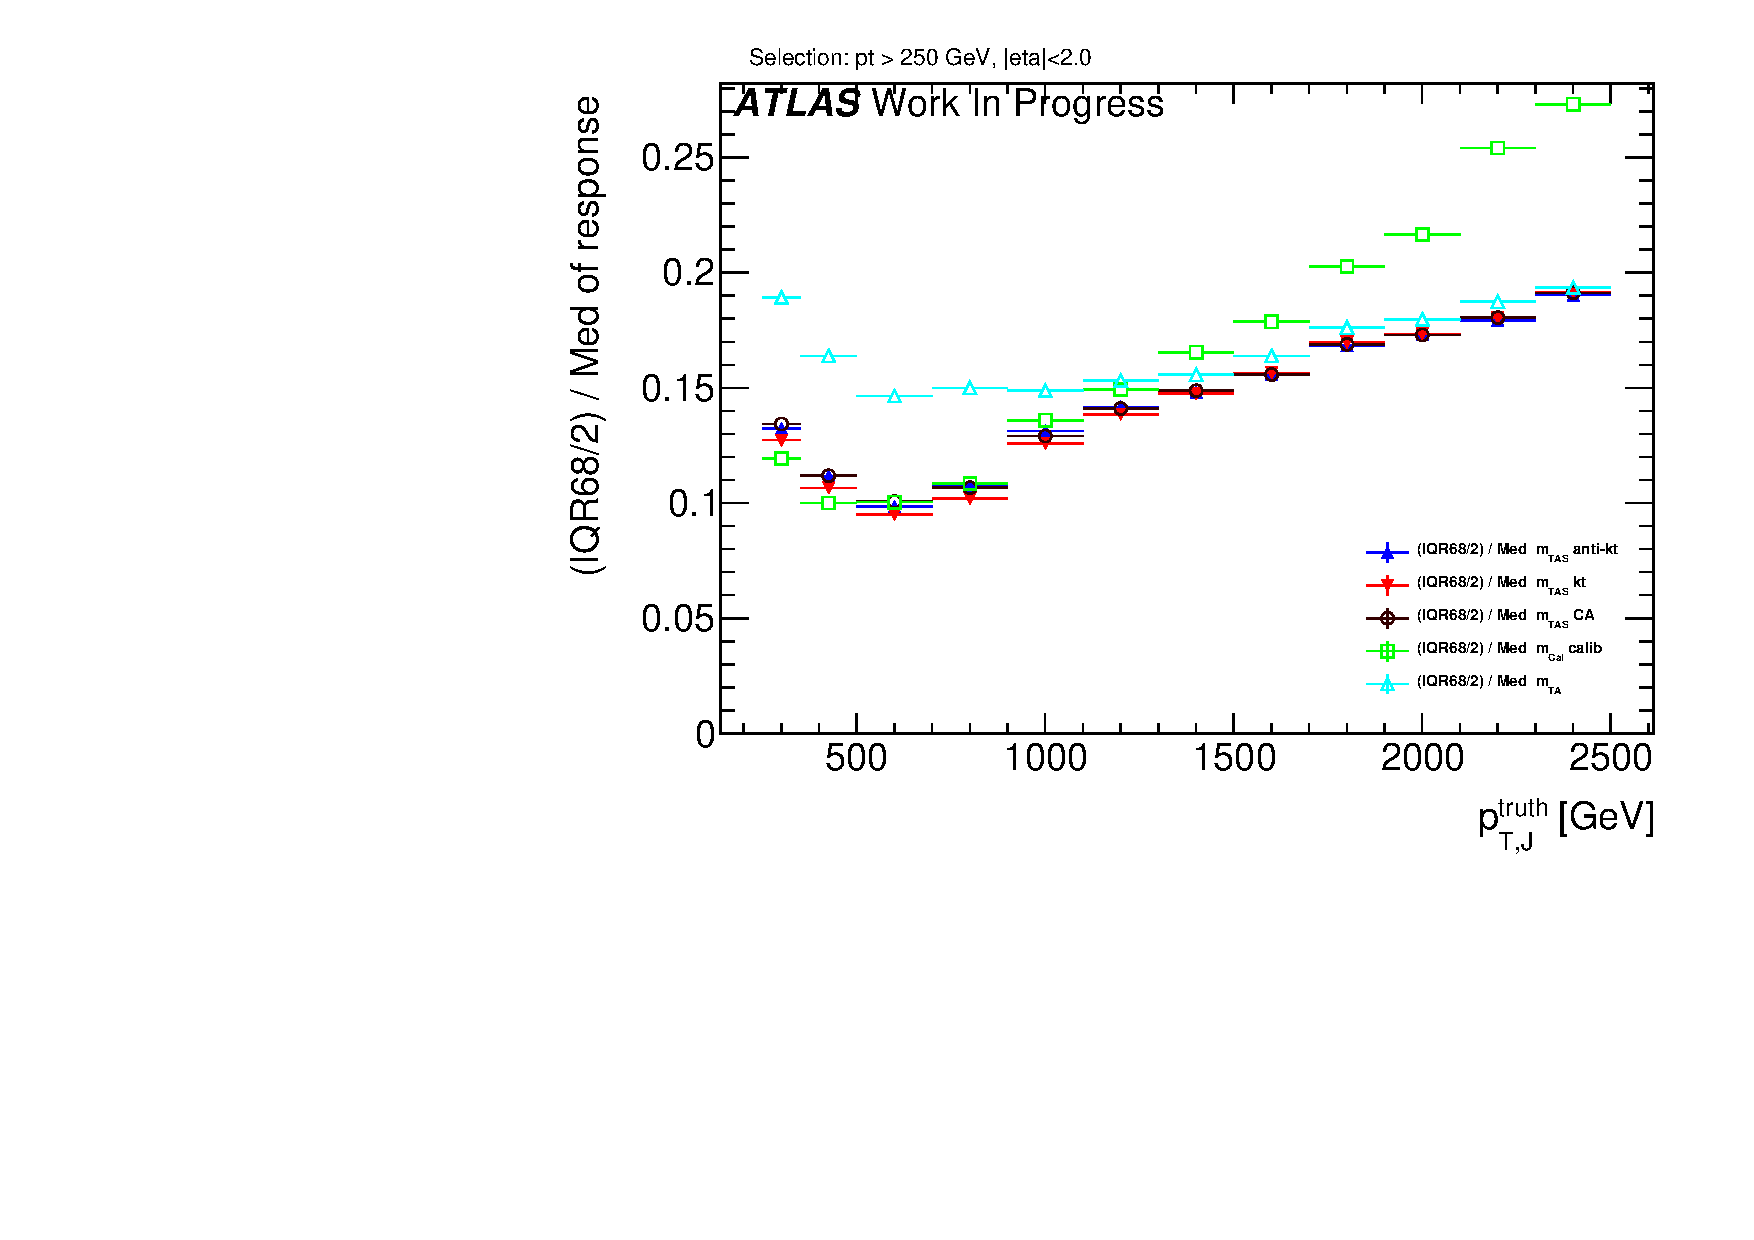
\includegraphics[width=\textwidth]{jet_part/mtas/71graphcftr_h_JetRatio_mJ12CALOIQRoM_Wprime_Allalgos.pdf}
   
%     \caption{Performance of $\mtas$ with different reclustering algorithm for the sub-jets: anti-k$_t$, k$_t$ and C/A. Boosted $W/Z$ sample.}
%     \label{fig:allalgow}
% \end{figure}

% \begin{figure}
%     \centering
%    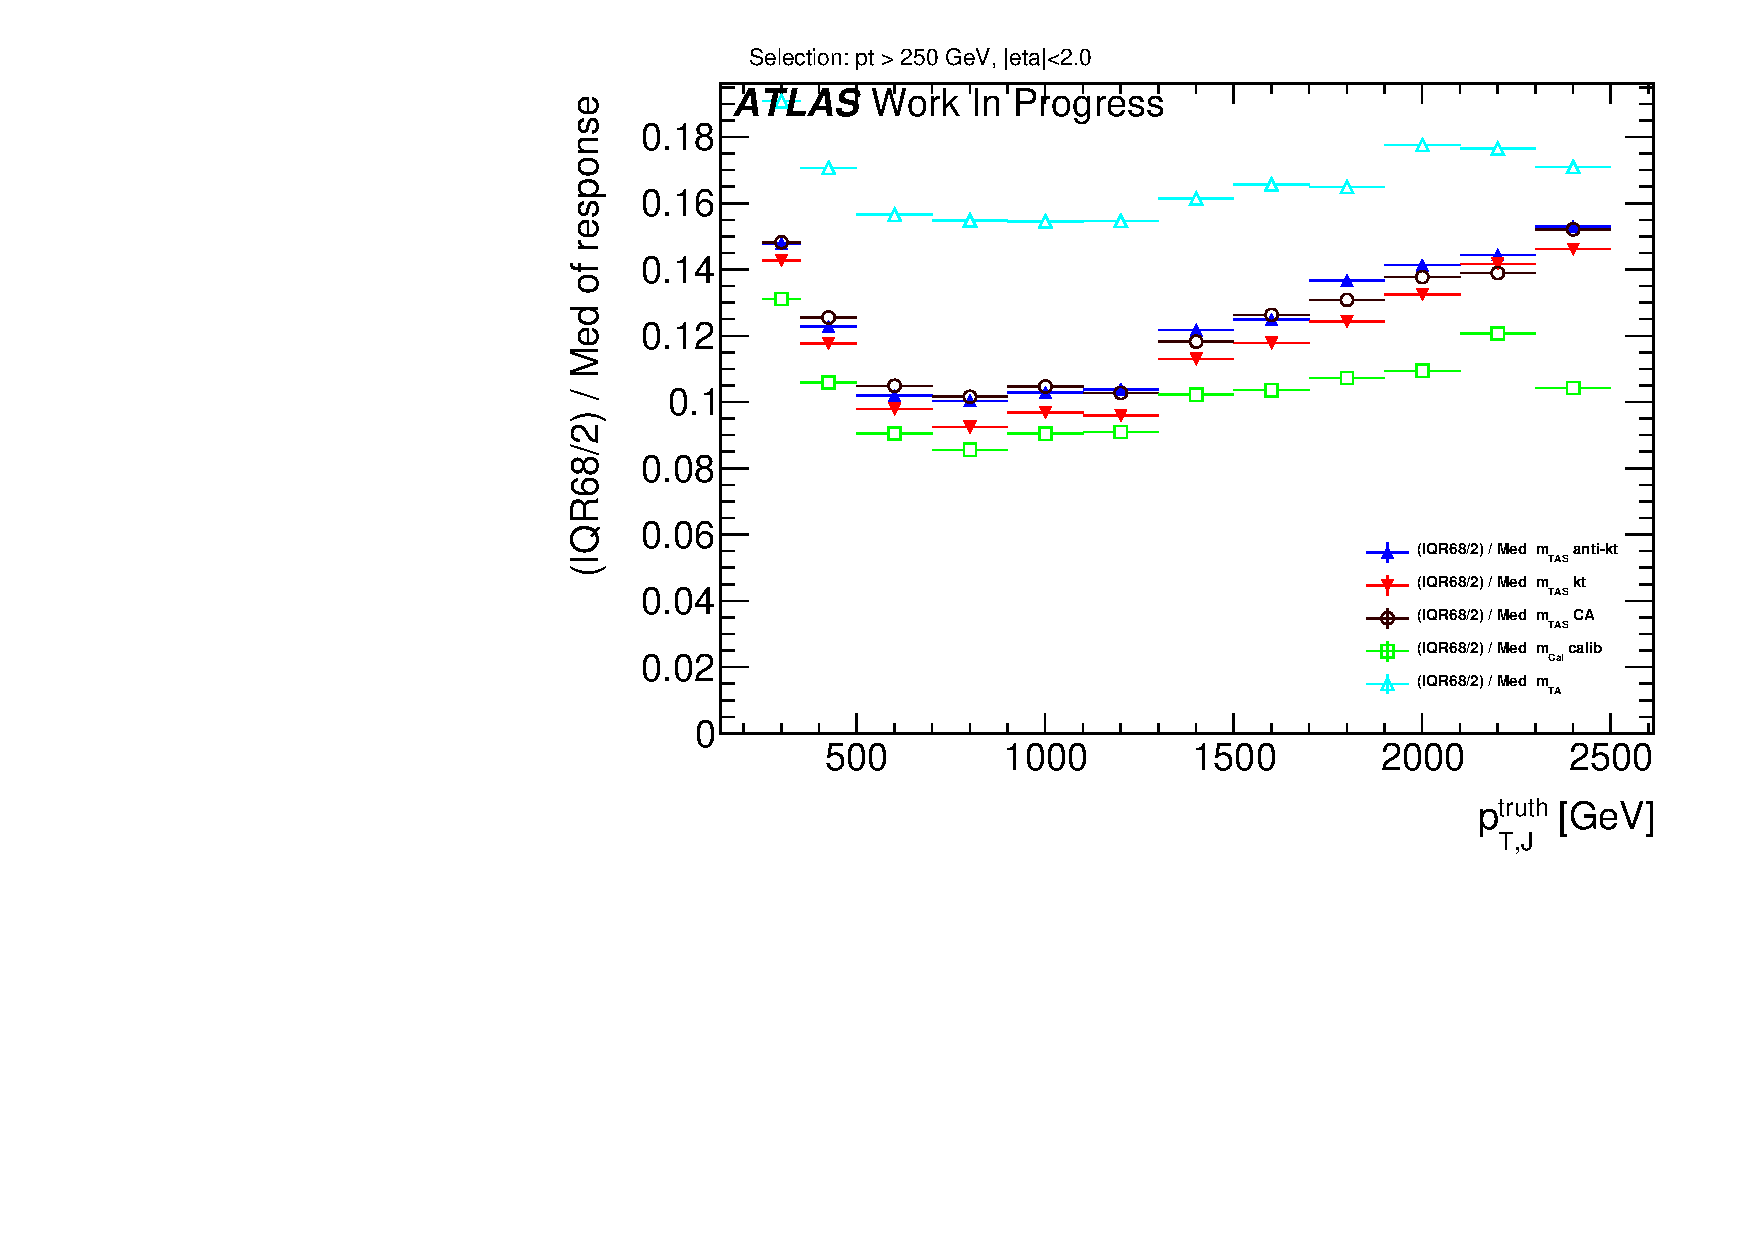
\includegraphics[width=\textwidth]{jet_part/mtas/71graphcftr_h_JetRatio_mJ12CALOTopsCalib.pdf}
   
%     \caption{Performance of $\mtas$ with different reclustering algorithm for the sub-jets: anti-k$_t$, k$_t$ and C/A. Boosted top sample.}
%     \label{fig:allalgotop}
% \end{figure}

% \begin{figure}
%     \centering
%    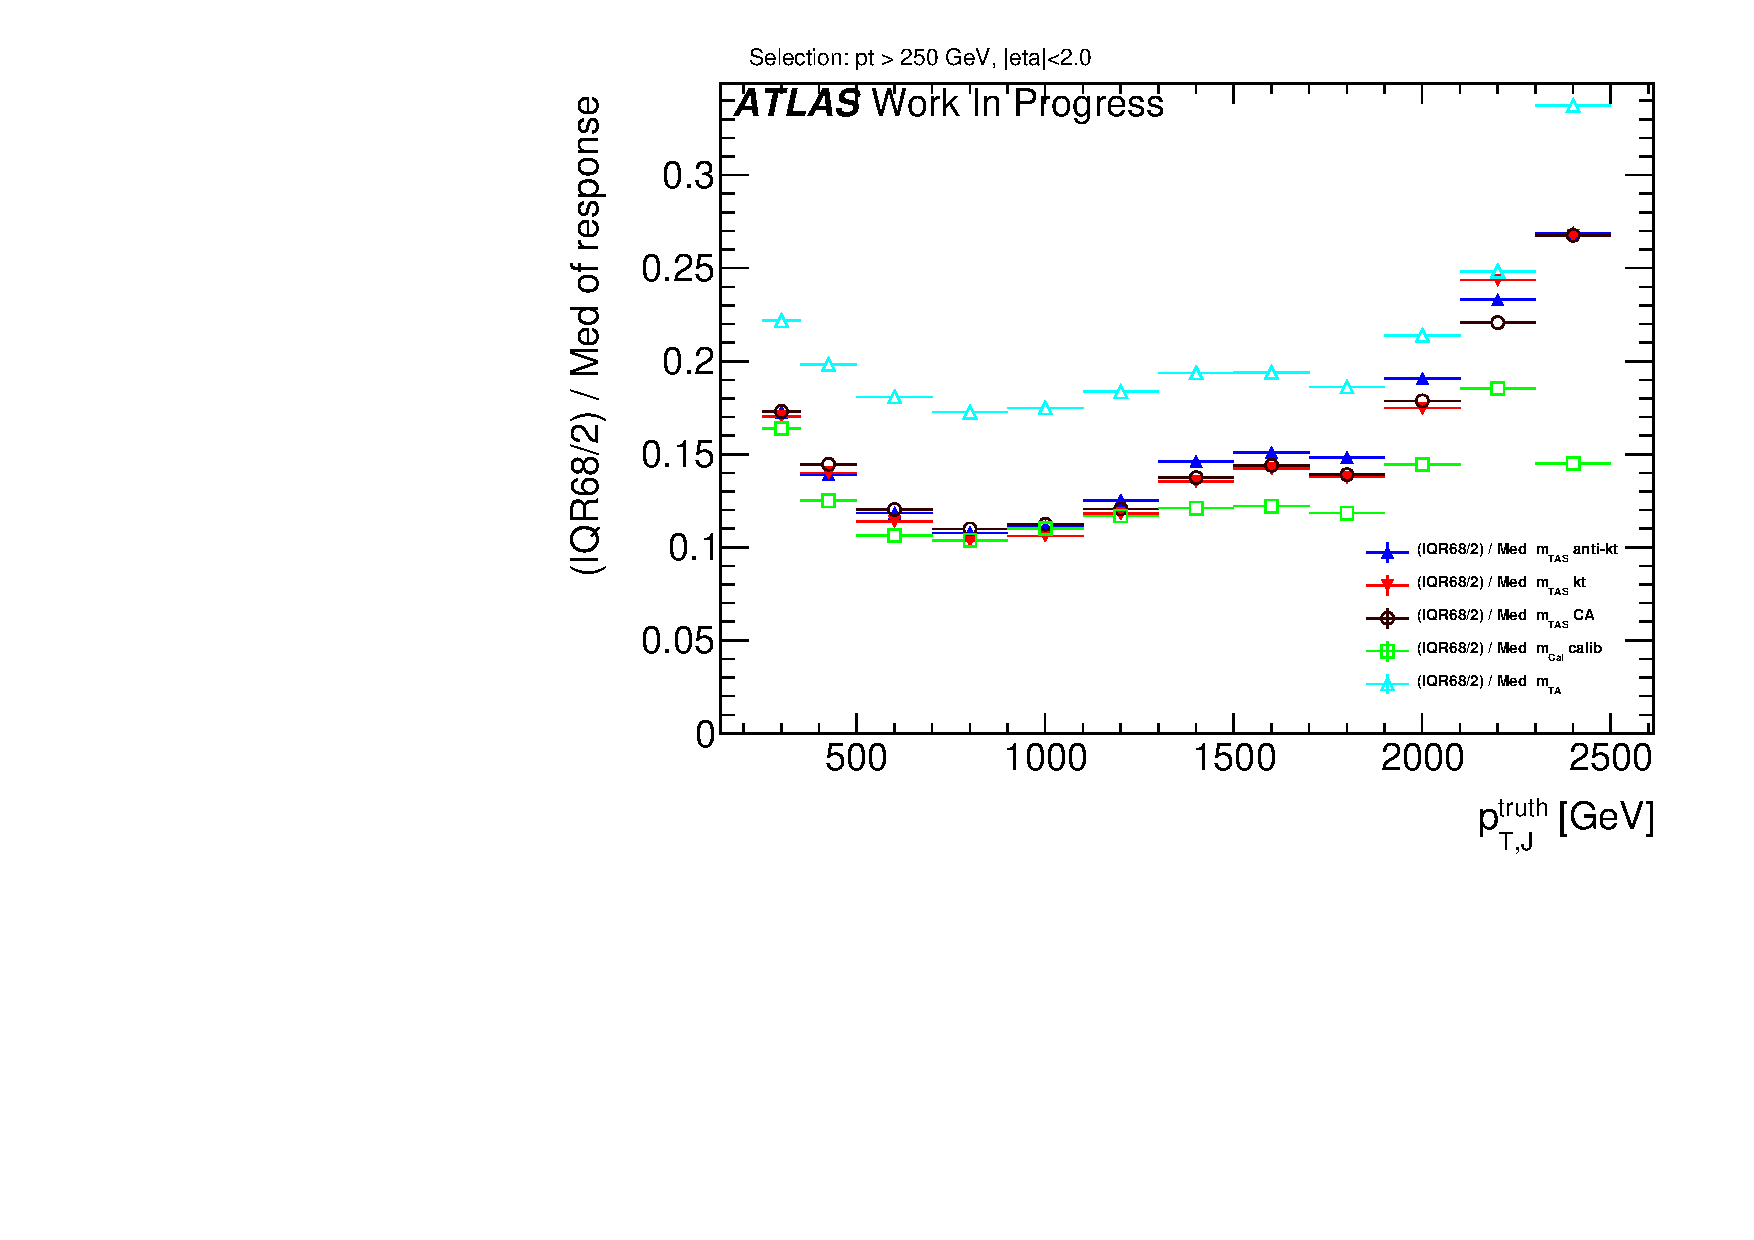
\includegraphics[width=\textwidth]{jet_part/mtas/71graphcftr_h_JetRatio_mJ12CALOIQRoMHiggsNOCalib.pdf}
   
%     \caption{Performance of $\mtas$ with different reclustering algorithm for the sub-jets: anti-k$_t$, k$_t$ and C/A. Boosted higgs sample.}
%     \label{fig:allalgohiggs}
% \end{figure}
\clearpage
\section{Performance of Combined Calorimeter and Track-Assisted Sub-Jet Mass}
This section presents the achievement of the variable obtained combining the $\mtas$ and the $\mcal$, the $\mcombtas$ with respect to the combination of the $\mta$ and the $\mcal$, the $\mcomb$. Both these variables were defined in \ref{subsec:comb}

\begin{figure}
    \centering
    \begin{subfigure}[b]{0.45\textwidth}
        \centering
   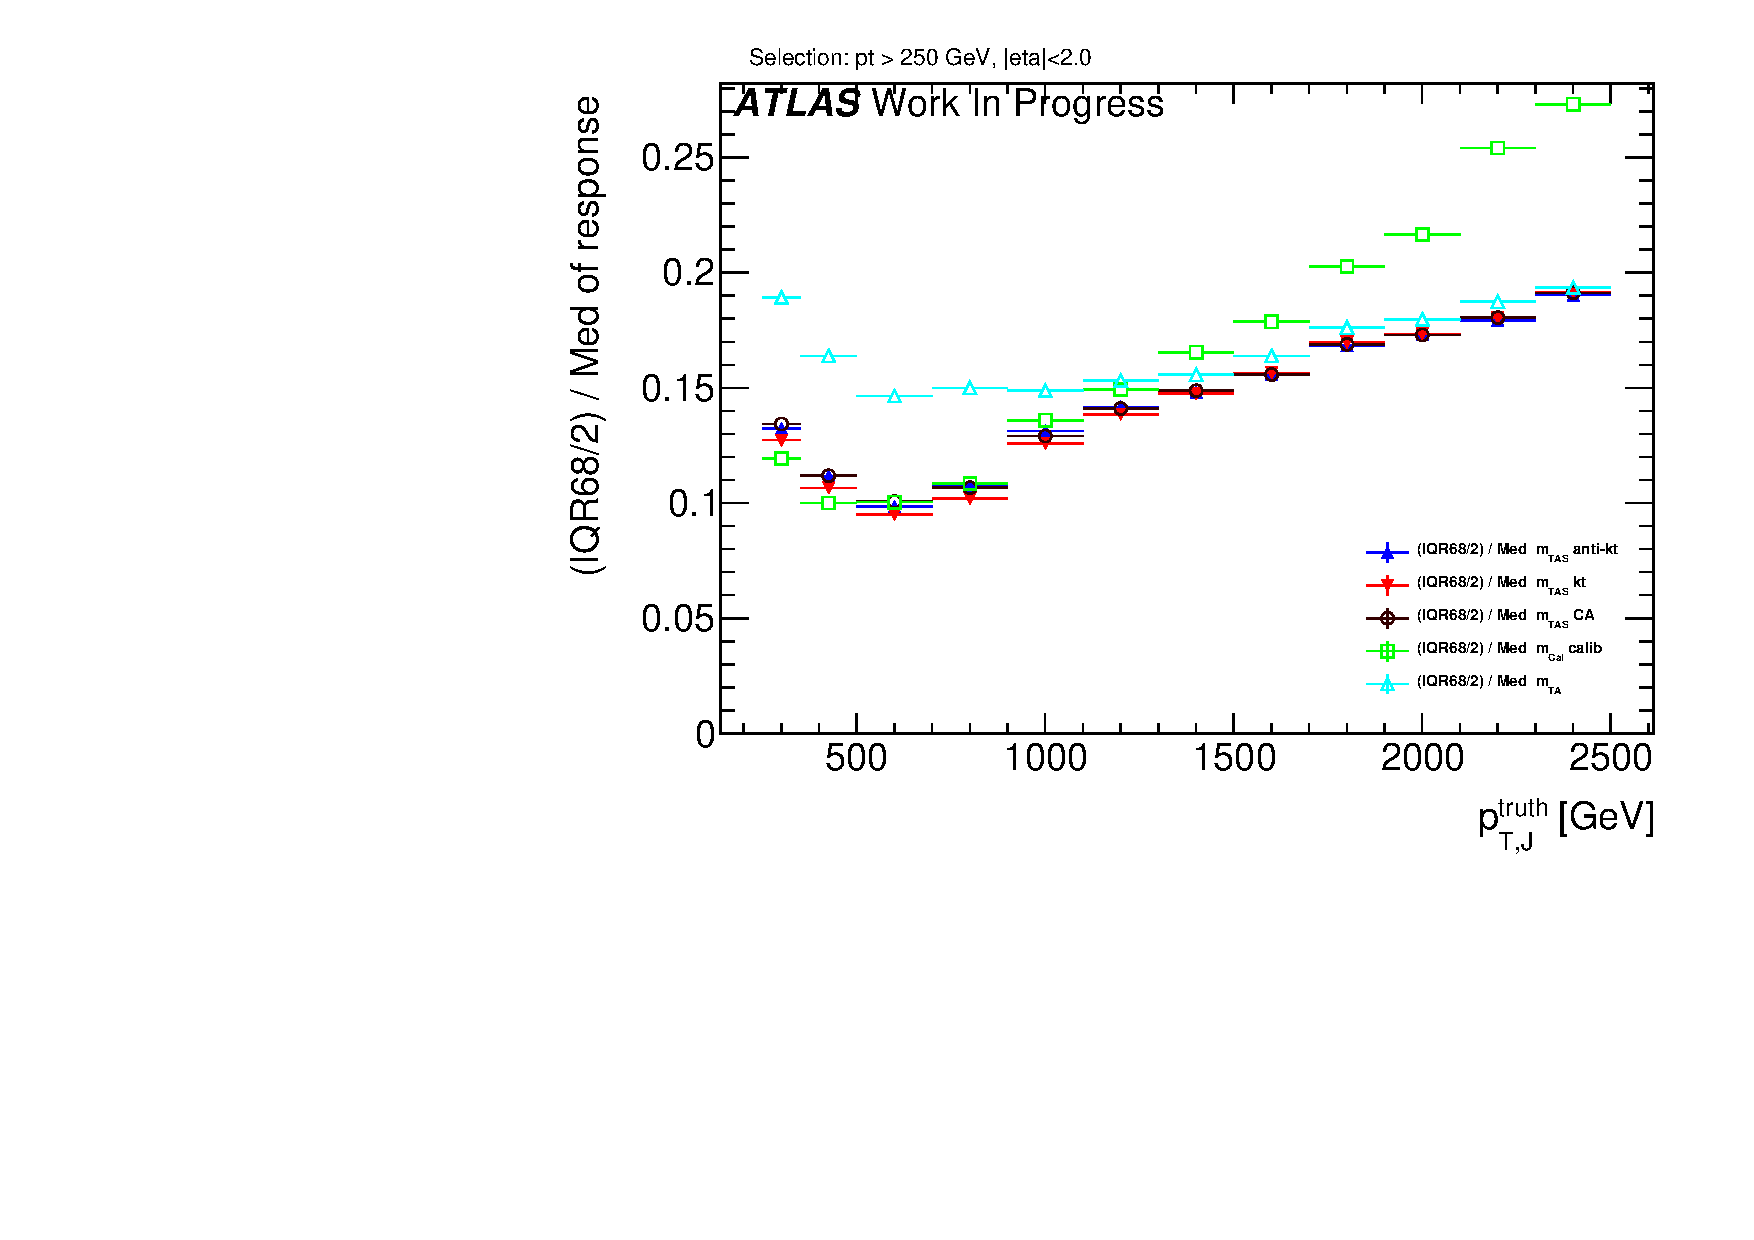
\includegraphics[width=\textwidth]{jet_part/mtas/71graphcftr_h_JetRatio_mJ12CALOIQRoM_Wprime_Allalgos.pdf}
    \caption{$W/Z$ jets.}
    \label{fig:allalgow}
    \end{subfigure}
    \begin{subfigure}[b]{0.45\textwidth}
        \centering
   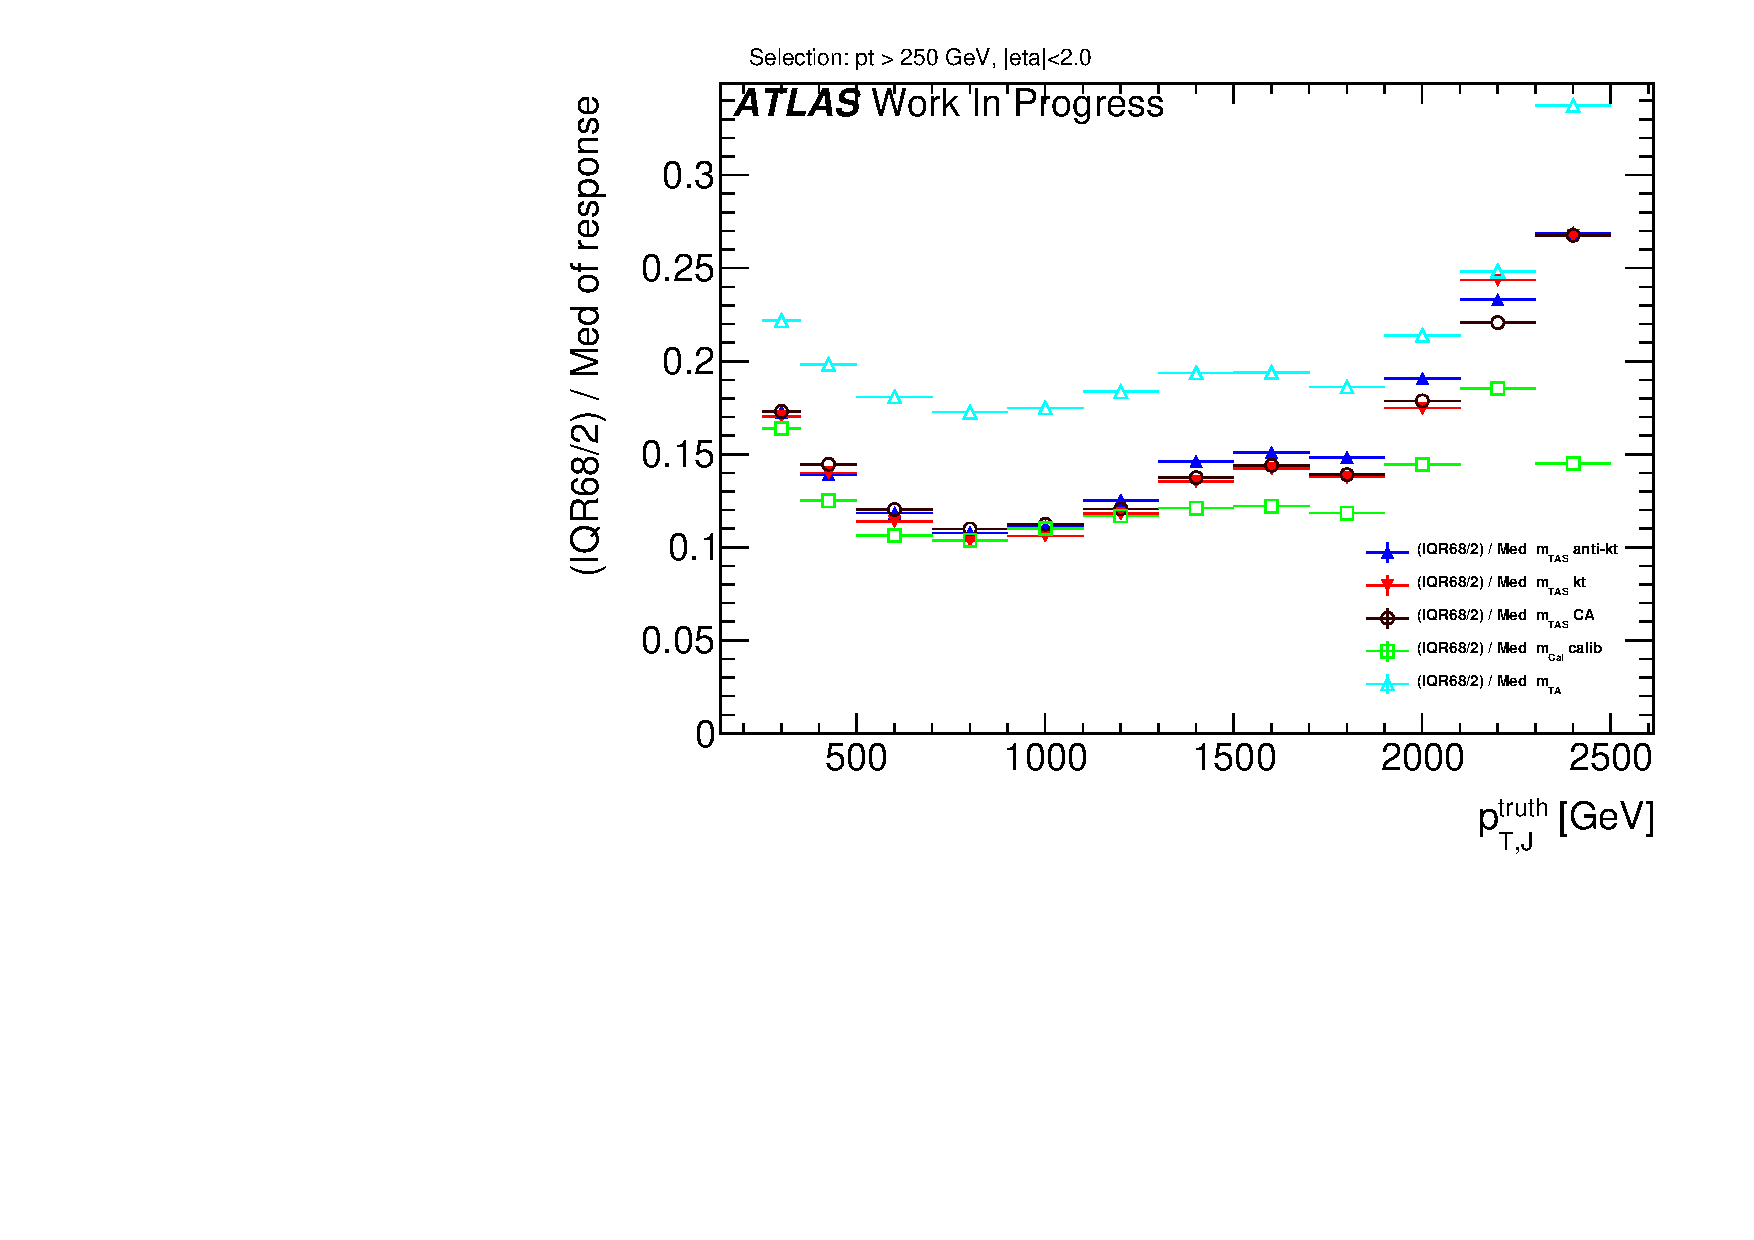
\includegraphics[width=\textwidth]{jet_part/mtas/71graphcftr_h_JetRatio_mJ12CALOIQRoMHiggsNOCalib.pdf}
    \caption{Higgs jets.}
    \label{fig:allalgohiggs}
    \end{subfigure}

    \begin{subfigure}[b]{0.45\textwidth}
        \centering
   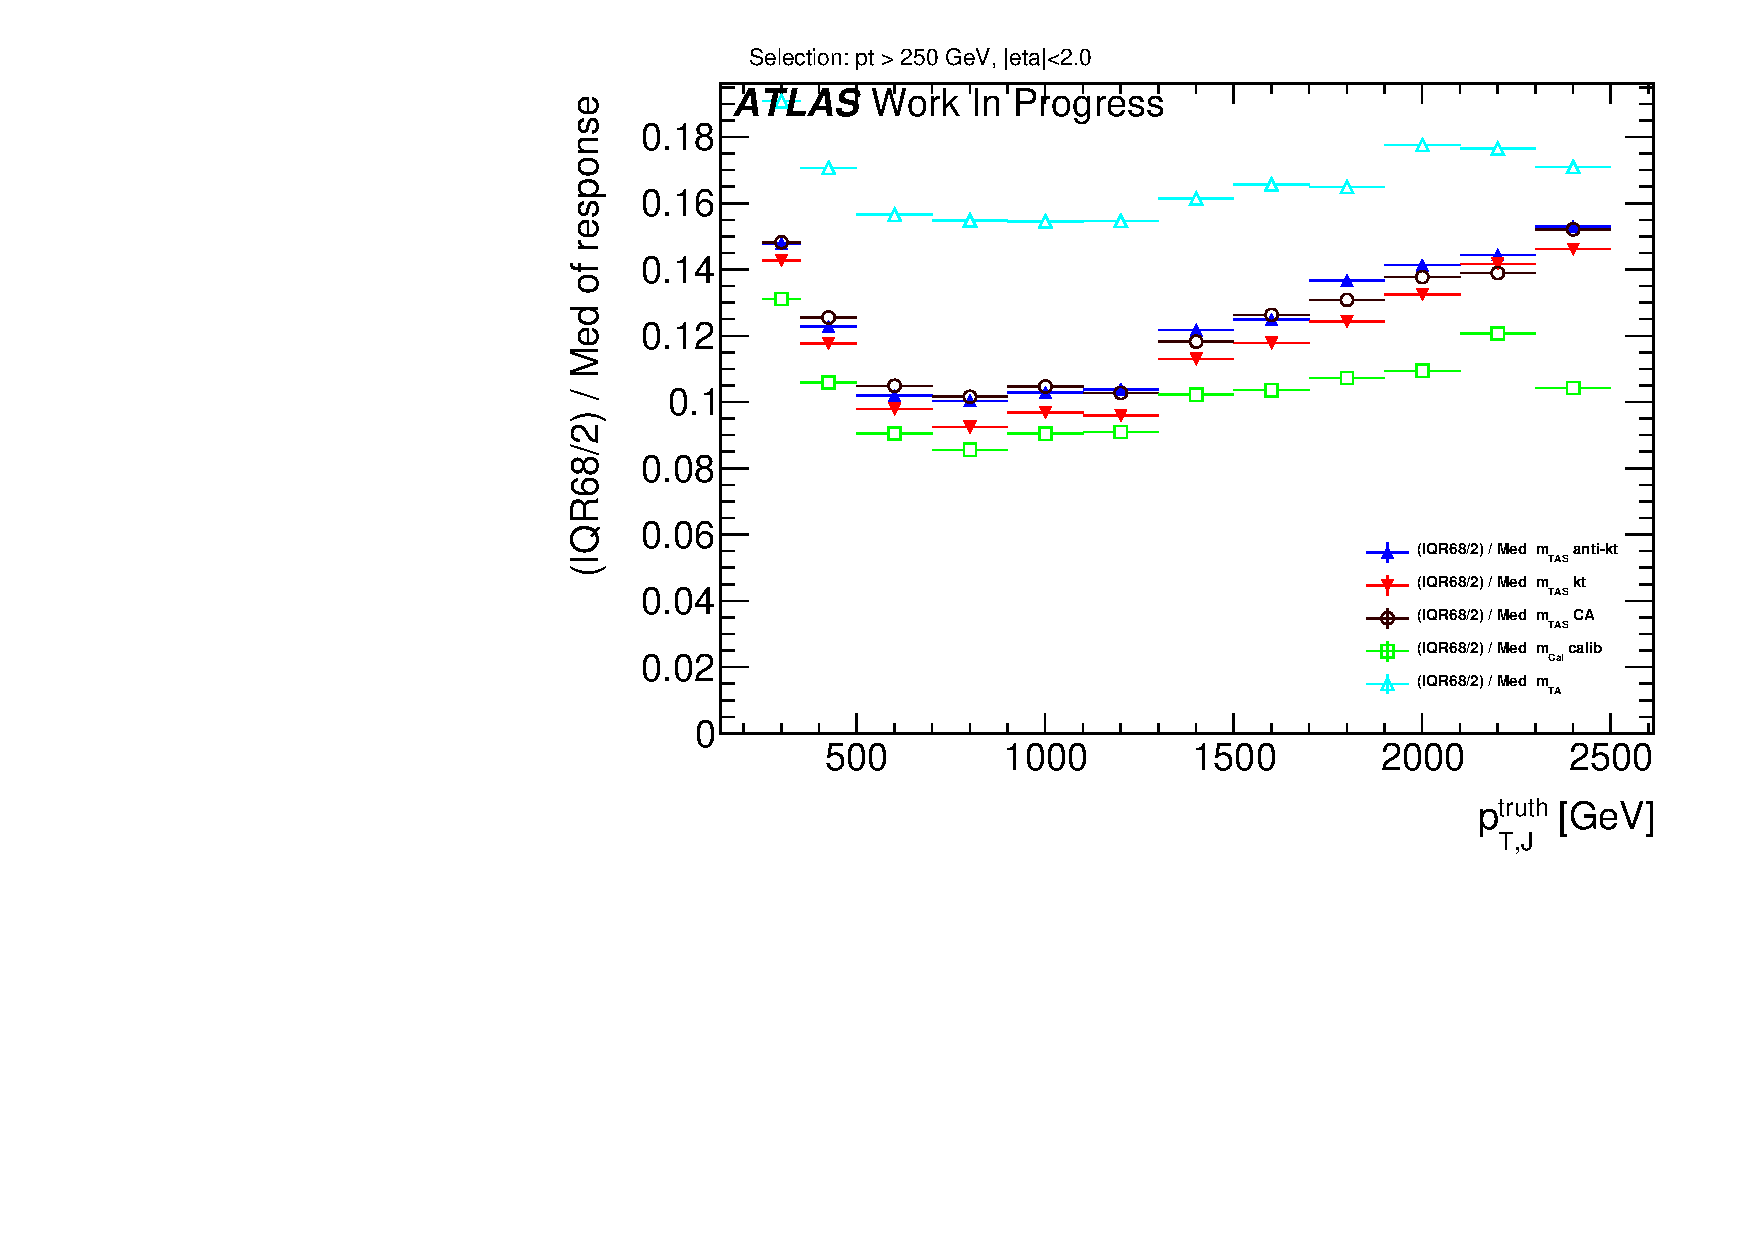
\includegraphics[width=\textwidth]{jet_part/mtas/71graphcftr_h_JetRatio_mJ12CALOTopsCalib.pdf}
    \caption{Top jets.}
    \label{fig:allalgotop}
    \end{subfigure}

\caption{Performance of $\mtas$ with different reclustering algorithms for the sub-jets: anti-k$_t$, k$_t$ and C/A and for $W/Z$ jets, top left, Higgs jets, top right and top jets, bottom. In all the cases shown, the k$_t$ is producing the better results, but all the three have a very similar performance.}
\end{figure}


\subsection{Performance in $W \to q'\bar{q}$ Decays}
On the $W/Z$s decays, the $\mcombtas$ outperforms all the other definitions throughout all the transverse momentum space; on Figure \ref{fig:mcombtas3} they are shown for reference together with the $\mtas$. It can be noted here that the track-assisted sub-jet mass, although being sub-optimal, has comparable performance, yet presenting fewer complications due to the combination procedure.

% \begin{figure}[!ht]
%   \centering
%       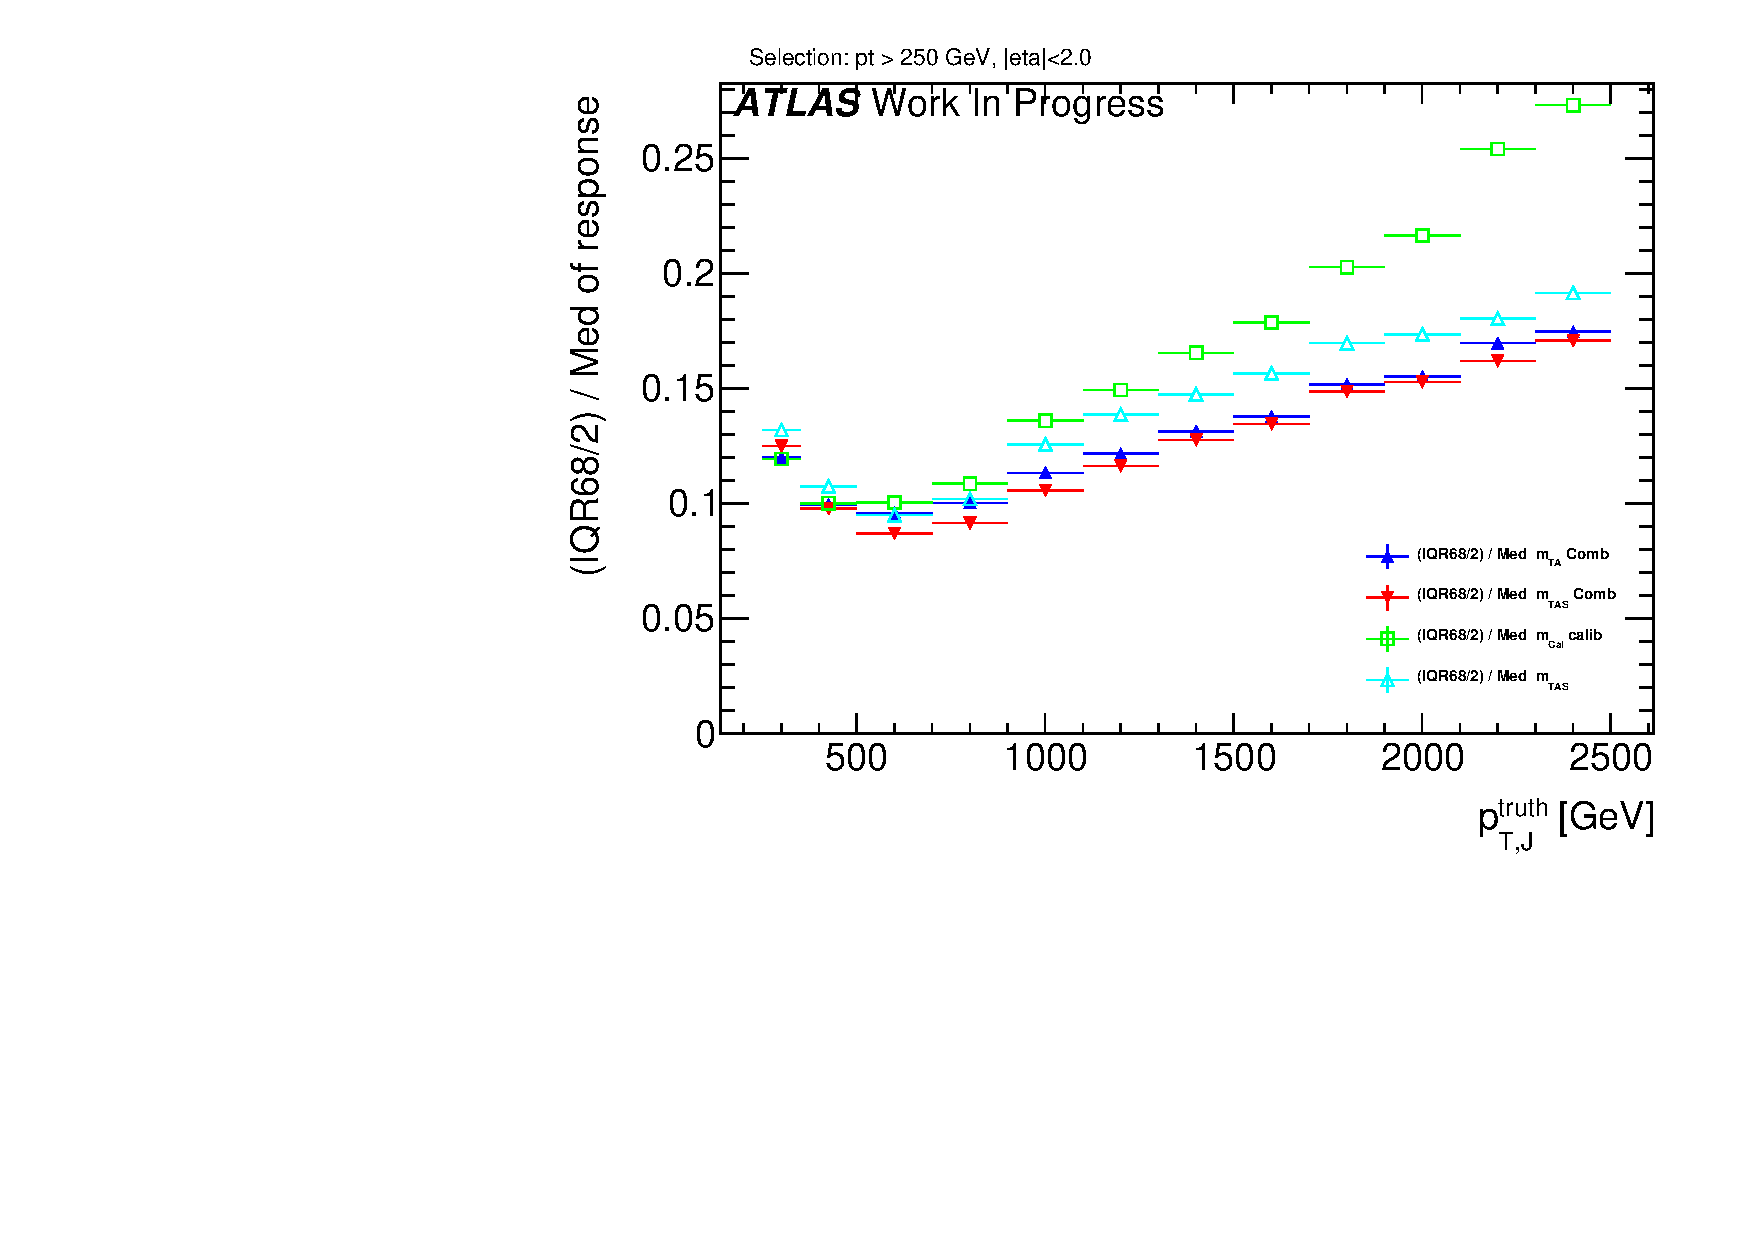
\includegraphics[width=0.7\textwidth]{jet_part/mcomb/mcombtas3.pdf}
%   \caption[$\mcombtas$ on the boosted $W/Z$]{Performance of the combined mass on $W/Z$ samples; here shown the two definitions of the combined mass, $\mcomb$ and $\mcombtas$, together with the calorimeter mass and the track-assisted sub-jet mass.}
%   \label{fig:mcombtas3}
% \end{figure}


\begin{figure}
    \centering
    \begin{subfigure}[b]{0.45\textwidth}
  \centering
      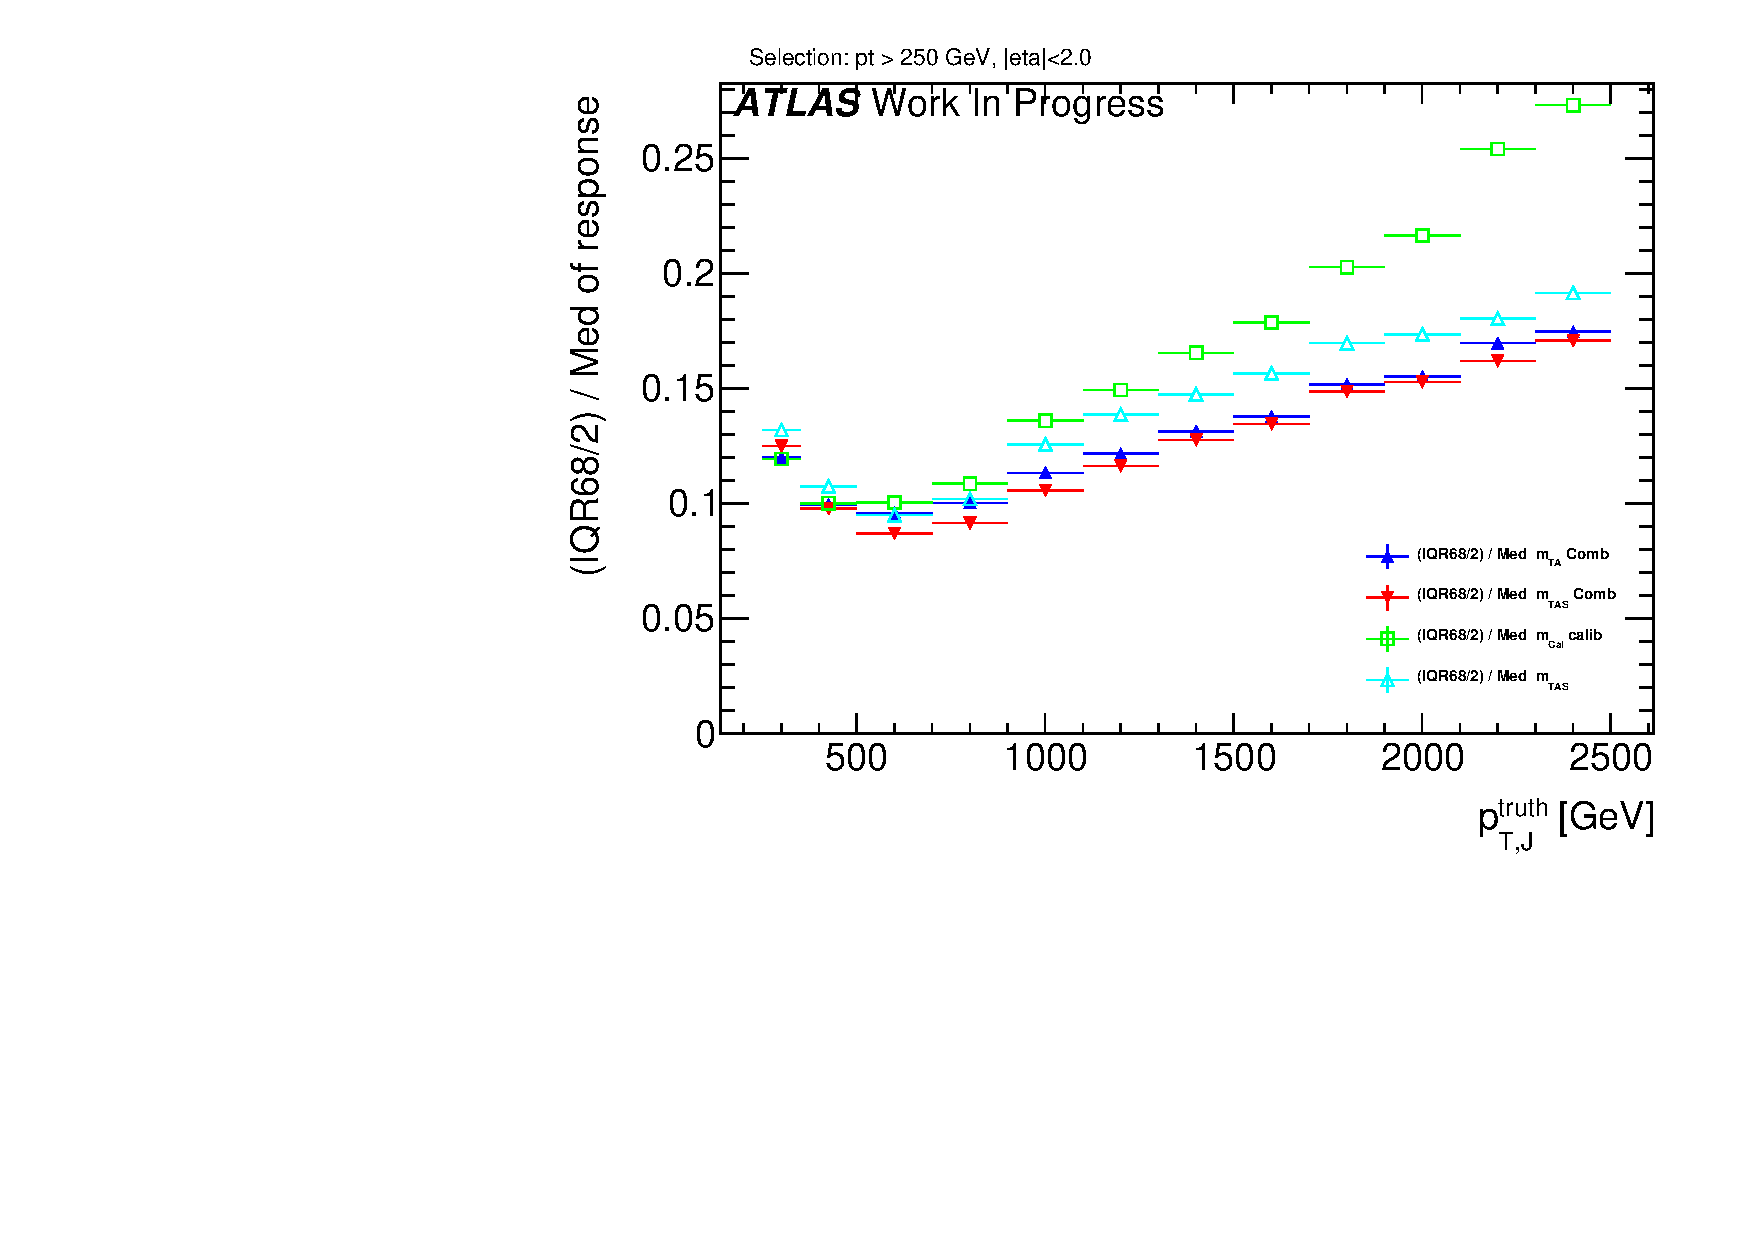
\includegraphics[width=0.9\textwidth]{jet_part/mcomb/mcombtas3.pdf}
  \caption[$\mcombtas$ on the boosted $W/Z$]{$W/Z$ jets.}
  \label{fig:mcombtas3}
    \end{subfigure}
    \begin{subfigure}[b]{0.45\textwidth}
  \centering
      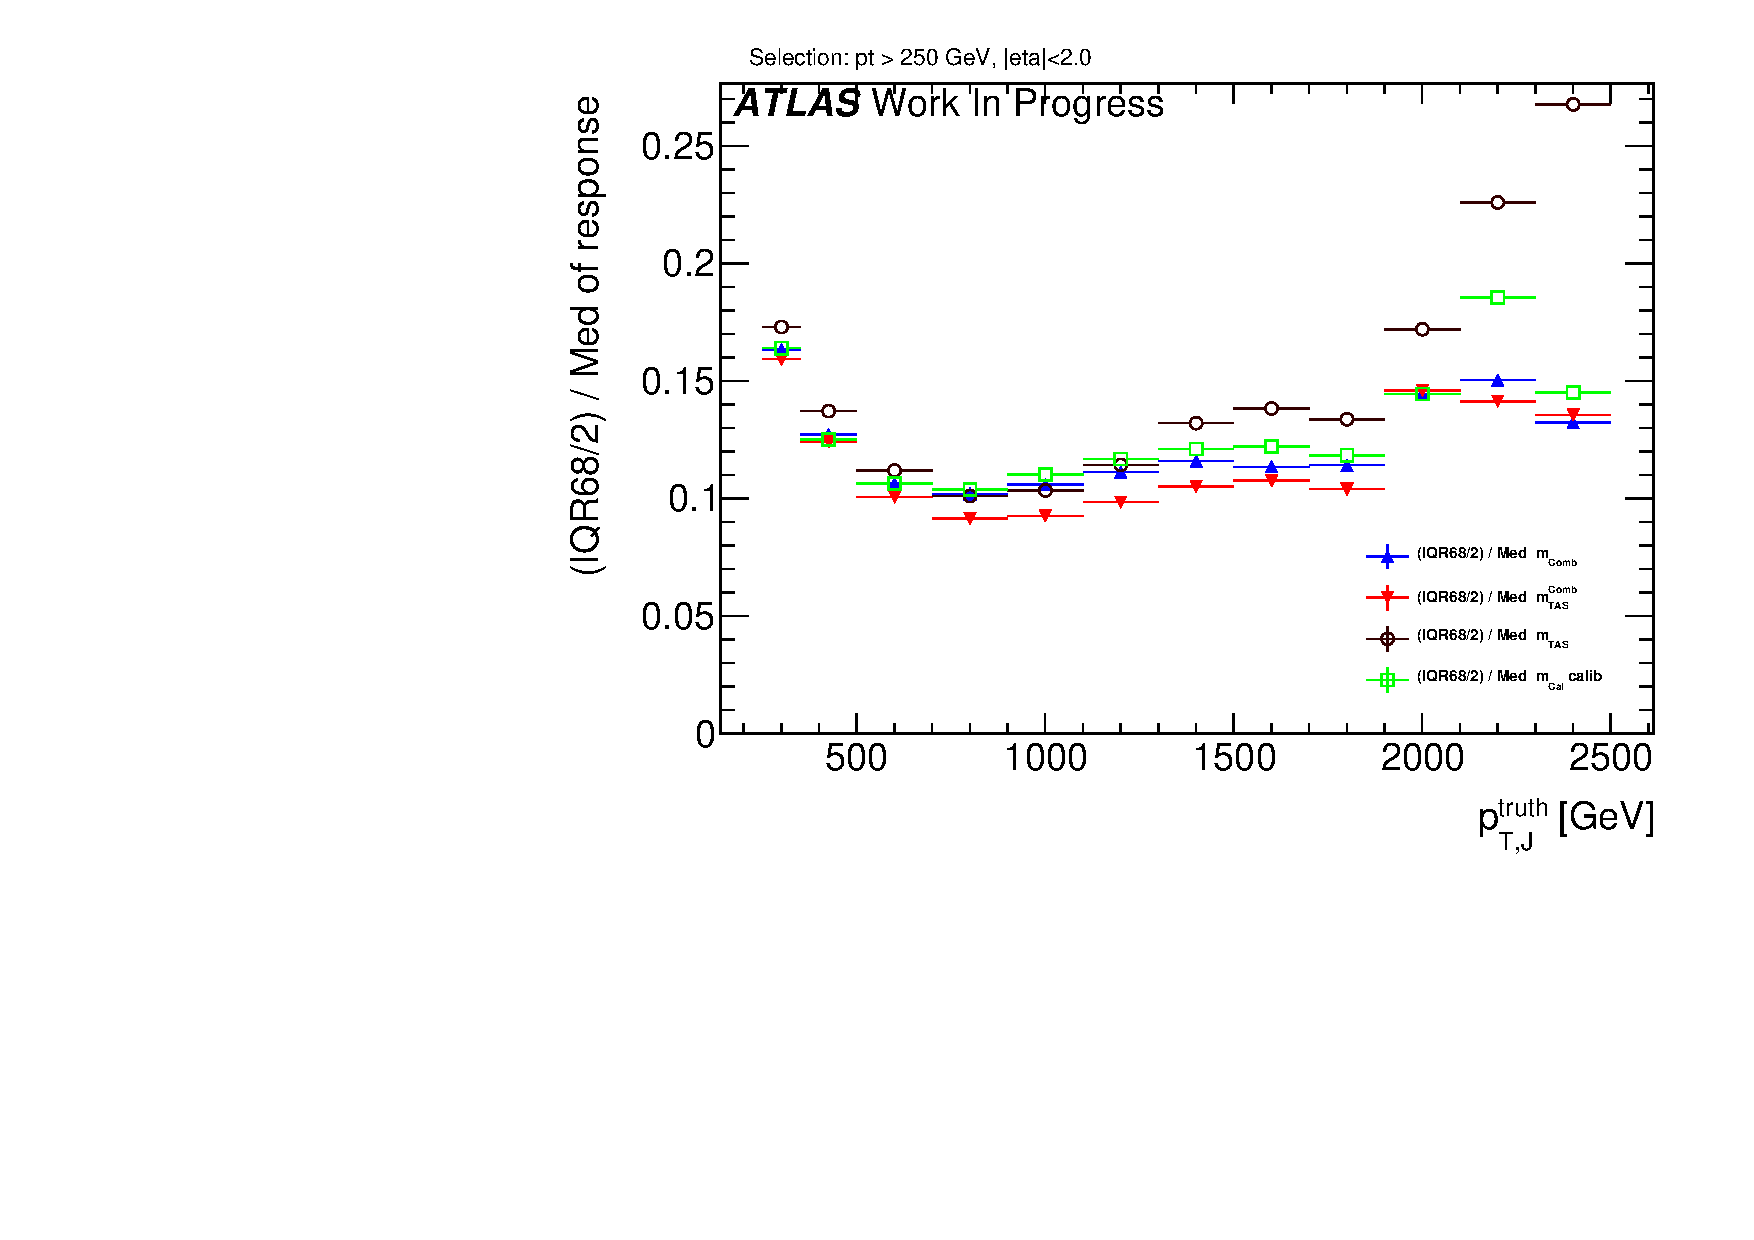
\includegraphics[width=0.9\textwidth]{jet_part/mcomb/mcombtas5.pdf}
  \caption[$\mcombtas$ on the boosted Higgs]{Higgs jets.}
  \label{fig:mcombtas5}
    \end{subfigure}

    \begin{subfigure}[b]{0.45\textwidth}
  \centering
      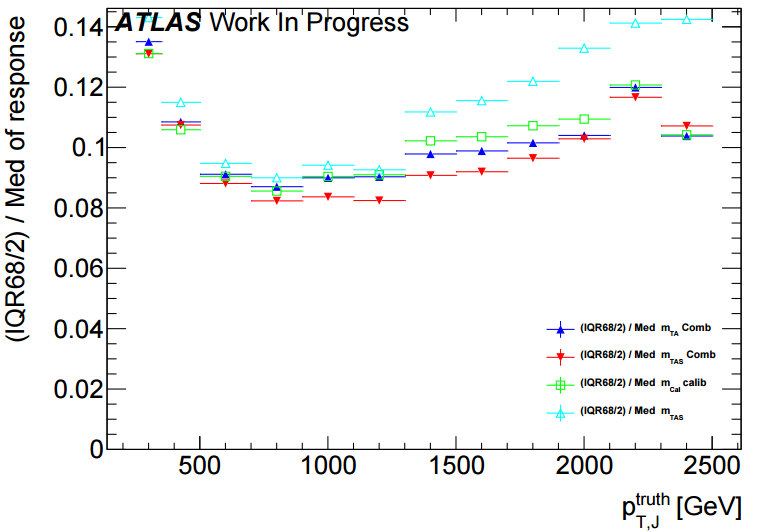
\includegraphics[width=0.9\textwidth]{jet_part/mcomb/mcombtas4.png}
  \caption[$\mcombtas$ on the boosted tops]{Top jets.}
  \label{fig:mcombtas4}
    \end{subfigure}
\caption{Performance of $\mcomb$ and $\mcombtas$ for different samples: the $W/Z$ jets, top left, the Higgs jets, top right and the top jets, bottom. The $\mcombtas$ outperforms the other definitions throughout the whole spectrum of transverse momentum. The $\mtas$, although being sub-optimal follows with similar performance the $\mcomb$. The Higgs and top jets presents the same properties as shown before, and the combined mass reflects these properties. }
\end{figure}

\subsection{Performance in $h\to b\bar{b}$ Decays}
Again, for the Higgs decay there are similarities as for the top sample; on Figure \ref{fig:mcombtas5} the two definitions of the combined mass, together with the simpler $\mtas$. Although this variable is slightly sub-optimal yet still comparable in the low to intermediate range in transverse momenta, where the tracks are driving a decrease in performance for the high to very-high $\pt$. The $\mcombtas$ uses this advantage to achieve optimal behavior in the entire transverse momentum spectrum, outperforming both $\mcal$ and $\mcomb$ almost everywhere.


\subsection{Performance in $t\to q'\bar{q}b$ Decays}
The top decay remains the most challenging phenomenon also with the combined mass; as seen on Figure \ref{fig:mcombtas4}, the $\mcomb$ performs quite similarly to the calorimeter based mass definition, yet behaving considerably better than the $\mtas$ especially at high transverse momentum. The $\mcombtas$, however, outperforms all the other definitions, and shows its optimal observable strength at intermediate $\pt$ i.e. in the range $0.8 < \pt < 1.6$ TeV.

% \begin{figure}[!ht]
%   \centering
%       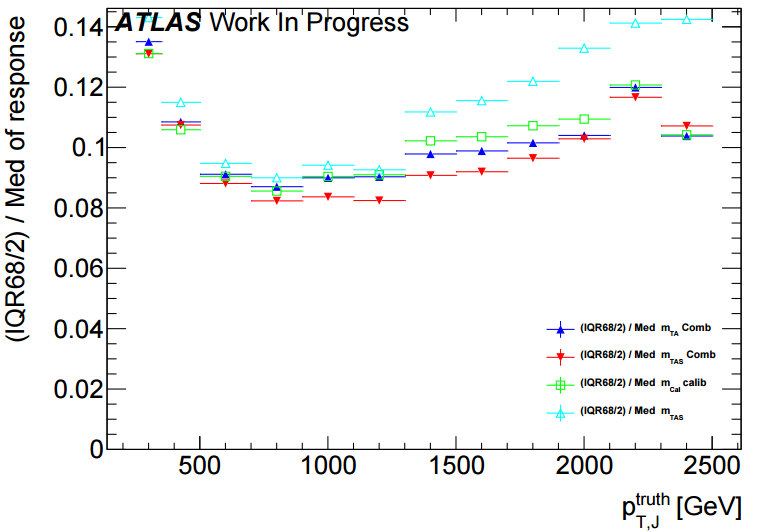
\includegraphics[width=0.7\textwidth]{jet_part/mcomb/mcombtas4.png}
%   \caption[$\mcombtas$ on the boosted tops]{Performance of the combined mass on the top sample; here shown the two definitions of the combined mass, $\mcomb$ and $\mcombtas$, together with the calorimeter mass and the track-assisted sub-jet mass.}
%   \label{fig:mcombtas4}
% \end{figure}

% \begin{figure}[!ht]
%   \centering
%       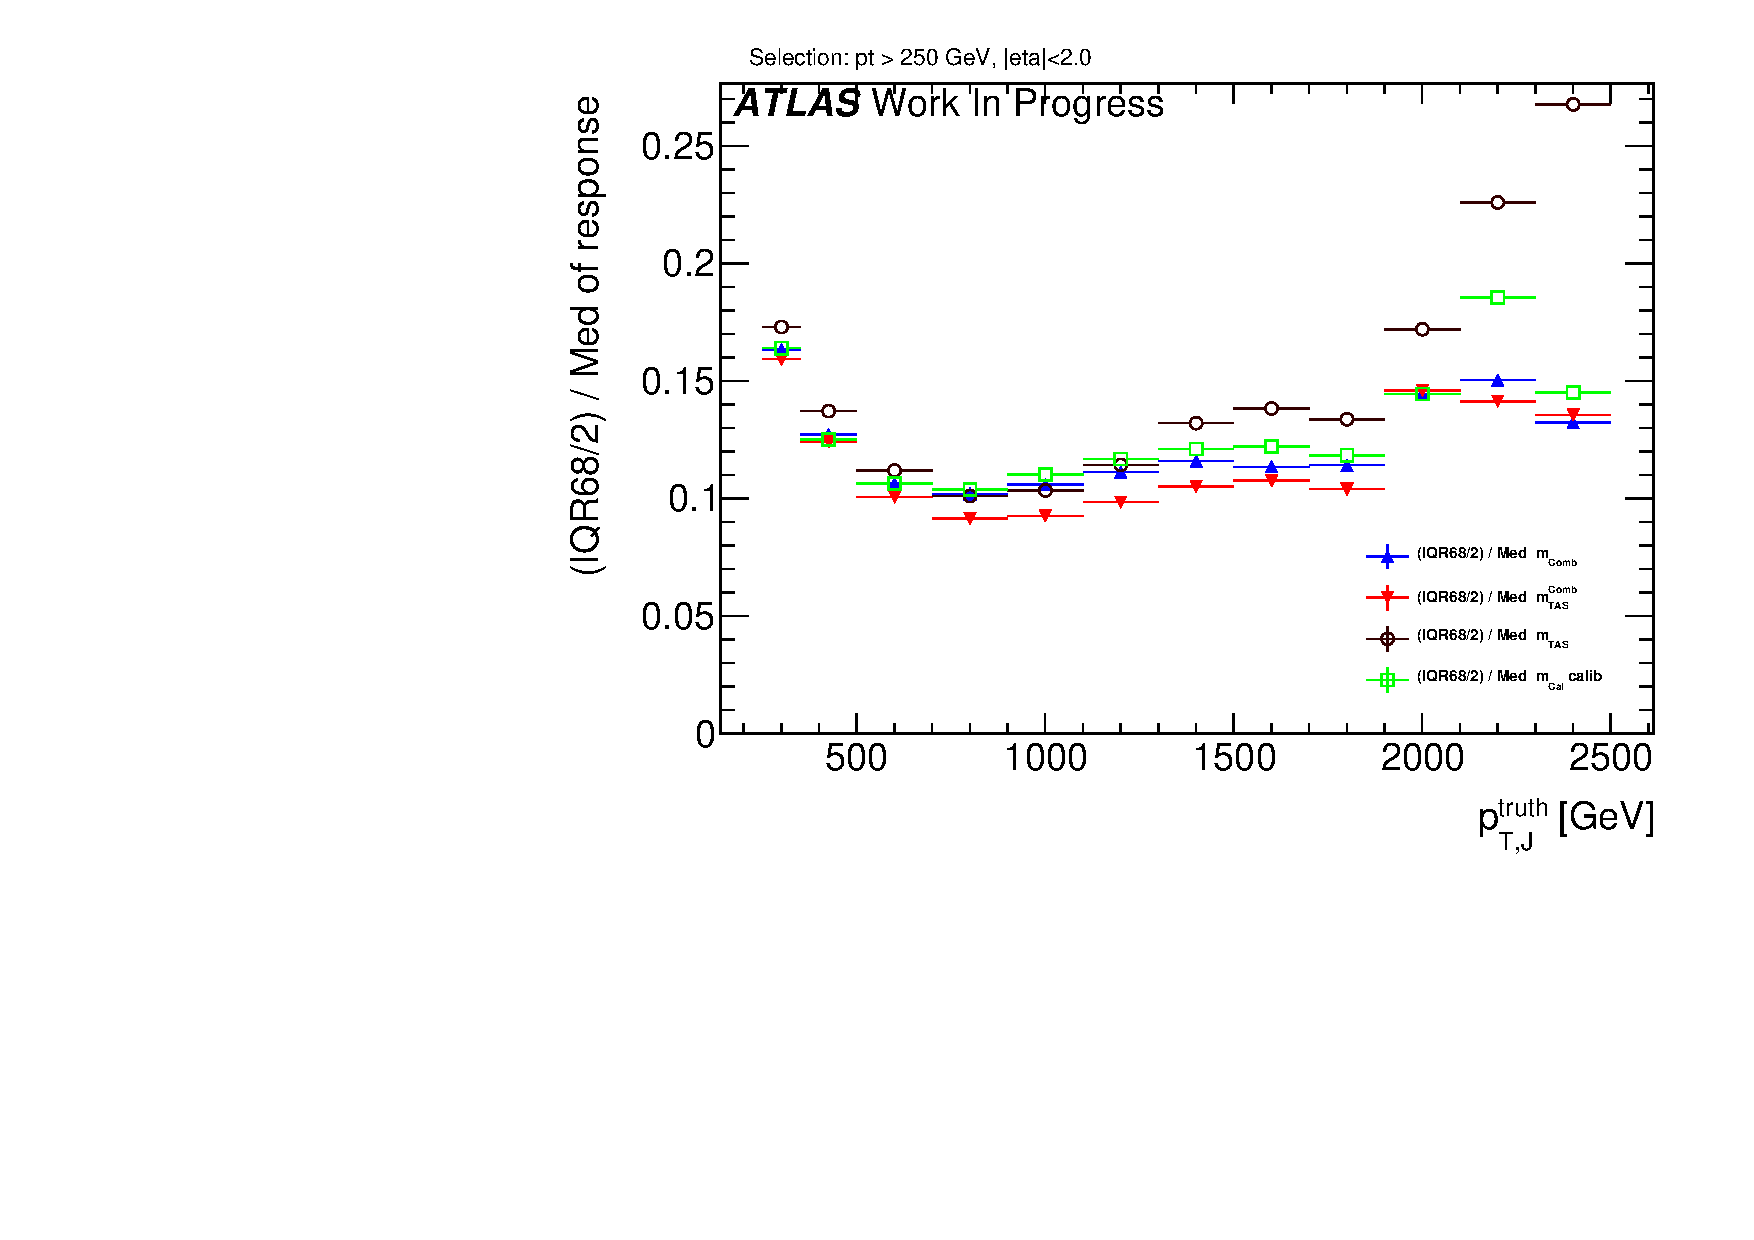
\includegraphics[width=0.7\textwidth]{jet_part/mcomb/mcombtas5.pdf}
%   \caption[$\mcombtas$ on the boosted Higgs]{Performance of the combined mass on the Higgs decay; here shown the two definitions of the combined mass, $\mcomb$ and $\mcombtas$, together with the calorimeter mass and the track-assisted sub-jet mass.}
%   \label{fig:mcombtas5}
% \end{figure}






